\documentclass[12pt]{ociamthesis}  % default square logo 
%\documentclass[12pt,beltcrest]{ociamthesis} % use old belt crest logo
%\documentclass[12pt,shieldcrest]{ociamthesis} % use older shield crest logo

%load any additional packages
\usepackage{amssymb}
\usepackage{listings}

%input macros (i.e. write your own macros file called mymacros.tex 
%and uncomment the next line)
%\include{mymacros}

\title{Modul Praktikum \\[1ex]     %your thesis title,
        Kecerdasan Buatan}   %note \\[1ex] is a line break in the title

\author{Rolly Maulana Awangga}             %your name
\college{0410118609\\[5ex]
Applied Bachelor of Informatics Engineering}  %your college

%\renewcommand{\submittedtext}{change the default text here if needed}
\degree{Politeknik Pos Indonesia}     %the degree
\degreedate{Bandung 2019}         %the degree date

%end the preamble and start the document
\begin{document}

%this baselineskip gives sufficient line spacing for an examiner to easily
%markup the thesis with comments
\baselineskip=18pt plus1pt

%set the number of sectioning levels that get number and appear in the contents
\setcounter{secnumdepth}{3}
\setcounter{tocdepth}{3}


\maketitle                  % create a title page from the preamble info
\begin{dedication}
`Jika Kamu tidak dapat menahan lelahnya belajar, \\
Maka kamu harus sanggup menahan perihnya Kebodohan.'\\ 
~Imam Syafi'i~\\
\end{dedication}        % include a dedication.tex file
\begin{acknowledgements}
Pertama-tama kami panjatkan puji dan syukur kepada Allah SWT yang telah memberikan rahmat dan hidayah-Nya sehingga Buku Pedoman Tingkat Akhir ini dapat diselesaikan.
\end{acknowledgements}   % include an acknowledgements.tex file
\begin{abstract}
	Buku Pedoman ini dibuat dengan tujuan memberikan acuan, bagi mahasiswa Tingkat Akhir dan dosen
	Pembimbing. Pada intinya buku ini menjelaskan secara lengkap tentang Standar pengerjaan Intership  dan 
	Tugas Akhir
	di Program Studi D4 Teknik Informatika, dan juga mengatur mekanisme, teknik penulisan, serta
	penilaiannya.Dengan demikian diharapkan semua pihak yang terlibat dalam aktivitas Bimbingan Mahasiswa Tingkat Akhir
	berjalan lancar dan sesuai dengan standar.
\end{abstract}          % include the abstract

\begin{romanpages}          % start roman page numbering
\tableofcontents            % generate and include a table of contents
\listoffigures              % generate and include a list of figures
\end{romanpages}            % end roman page numbering

%now include the files of latex for each of the chapters etc
\chapter{Mengenal Kecerdasan Buatan dan Scikit-Learn}
Buku umum yang digunakan adalah \cite{russell2016artificial} dan
untuk sebelum UTS menggunakan buku \textit{Python Artificial Intelligence Projects for Beginners}\cite{eckroth2018python}.
Dengan praktek menggunakan python 3 dan editor anaconda dan library python scikit-learn.
Tujuan pembelajaran pada pertemuan pertama antara lain:
\begin{enumerate}
\item
Mengerti definisi kecerdasan buatan, sejarah kecerdasan buatan, perkembangan dan penggunaan di perusahaan
\item
Memahami cara instalasi dan pemakaian sci-kit learn
\item
Memahami cara penggunaan variabel explorer di spyder
\end{enumerate}
Tugas dengan cara dikumpulkan dengan pull request ke github dengan menggunakan latex pada repo yang dibuat oleh asisten riset.

\section{Teori}
Praktek teori penunjang yang dikerjakan :
\begin{enumerate}
\item
Buat Resume Definisi, Sejarah dan perkembangan Kecerdasan Buatan, dengan bahasa yang mudah dipahami dan dimengerti. Buatan sendiri bebas plagiat[hari ke 1](10)
\item
Buat Resume mengenai definisi supervised learning, klasifikasi, regresi dan unsupervised learning. Data set, training set dan testing set.[hari ke 1](10)
\end{enumerate}

\section{Instalasi}
Membuka https://scikit-learn.org/stable/tutorial/basic/tutorial.html. Dengan menggunakan bahasa yang mudah dimengerti dan bebas plagiat.
Dan wajib skrinsut dari komputer sendiri.
\begin{enumerate}
\item
Instalasi library scikit dari anaconda, mencoba kompilasi dan uji coba ambil contoh kode dan lihat variabel explorer[hari ke 1](10)
\item
Mencoba Loading an example dataset, menjelaskan maksud dari tulisan tersebut dan mengartikan per baris[hari ke 1](10)
\item
Mencoba Learning and predicting, menjelaskan maksud dari tulisan tersebut dan mengartikan per baris[hari ke 2](10)
\item
mencoba Model persistence, menjelaskan maksud dari tulisan tersebut dan mengartikan per baris[hari ke 2](10)
\item
Mencoba Conventions, menjelaskan maksud dari tulisan tersebut dan mengartikan per baris[hari ke 2](10)
\end{enumerate}


\section{Penanganan Error}
Dari percobaan yang dilakukan di atas, apabila mendapatkan error maka:

\begin{enumerate}
	\item
	skrinsut error[hari ke 2](10)
	\item
Tuliskan kode eror dan jenis errornya [hari ke 2](10)
	\item
Solusi pemecahan masalah error tersebut[hari ke 2](10)

\end{enumerate}

\section{Fadila/1164072}
\subsection{Teori}
Teori mencakup resume dari beberapa pembahasan. yaitu :
\begin{enumerate}
\item Tentang Kecerdasan Buatan
\begin{itemize}
\item Definisi Kecerdasan Buatan.
\par Kecerdasan Buatan biasa disebut dengan istilah AI ( Artificial Intelligence ) . AI sendiri merupakan suatu cabang dalam bidang sains komputer sains dimana mengkaji tentang bagaimana cara untuk melengkapi sebuah komputer dengan kemampuan atau kepintaran layaknya atau mirip dengan yang dimiliki manusia. Sebagai contoh, sebagaimana komputer dapat berkomunikasi dengan pengguna baik menggunakan kata, suara maupun lain sebagainya . Dengan kemampuan ini, diharapkan komputer mampu mengambil keputusan sendiri untuk berbagai kasus yang ditemuinya kemudian itulah yang disebut dengan kecerdasan buatan.
\par  Kecerdasan buatan makin canggih dengan kemampuan komputer dalam memperbarui pengetahuannya dengan banyaknya testing dan perkembangan target analisa. Untuk kecerdasan buatan ada banyak contoh dan jenisnya. Salah satu contoh yang paling terkenal dari Artificial Intelligence ialah Google Assistant. Google Assistant digunakan untuk kemudahan user dalam menemukan berbagai hal maupun penyettingan langsung terhadap smartphone yang digunakan dan masih banyak lagi.
\item Sejarah Kecerdasan Buatan

\par Artificial intelligence merupakan inovasi baru di bidang ilmu pengetahuan. Mulai terbentuk sejak adanya komputer modern dan kira-kira terjadi sekitaran tahun 1940 dan 1950. Ilmu pengetahuan komputer ini khusus ditujukan dalam perancangan otomatisasi tingkah laku cerdas dalam sistem kecerdasan komputer.
\par Pada awalnya, kecerdasan buatan hanya ada di universitas-universitas dan laboratorium penelitian, serta hanya sedikit produk yang dihasilkan dan dikembangkan. Menjelang akhir 1970-an dan 1980-an, mulai dikembangkan secara penuh dan hasilnya berangsur-angsur dipublikasikan di khalayak umum.
\par

\begin{figure}[ht]
\centering
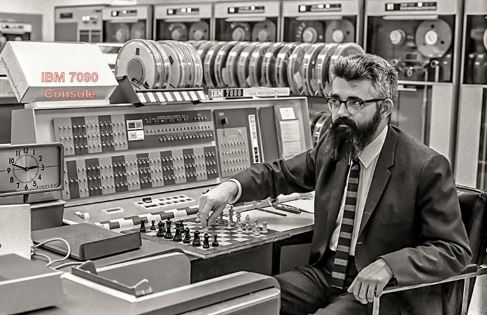
\includegraphics[scale=0.5]{figures/contoh.jpg}
\caption{capturing}
\label{contoh}
\end{figure}

\par Jika kita berbicara tentang AI atau Artificial Intelligence maka kita tidak bisa melupakan seorang sosok yang sangat terkenal pada bidang tersebut yaitu bapak John McCarthy.
McCarthy mendapatkan gelar sarjana matematika dari California Institute of Technology (Caltech) pada September 1948. Dari masa kuliahnya itulah ia mulai mengembangkan ketertarikannya pada mesin yang dapat menirukan cara berpikir manusia. McCarthy kemudian melanjutkan pendidikan ke program doktoral di Princeton University.

\par McCarthy kemudian mendirikan dua lembaga penelitian kecerdasan buatan. Kedua lembaga AI itu adalah Stanford Artificial Intelligence Laboratory dan MIT Artificial Inteligence Laboratory. Di lembaga-lembaga inilah bermunculan inovasi pengembangan AI yang meliputi bidang human skill, vision, listening, reasoning dan movement of limbs. Bahkan Salah satu lembaga yang didirikan itu, Stanford Artificial Intelligence pernah mendapat bantuan dana dari Pentagon untuk membuat teknologi-teknologi luar angkasa.

\item Perkembangan Kecerdasan Buatan
\par Teknologi Artificial Intelligence semakin ramai dibahas dalam berbagai diskusi teknologi di seluruh dunia.Menurut kebanyakan orang, pekerjaan seperti kasir, operator telepon, pengendara truk, dan lainnya sangat berpeluang besar untuk tergantikan oleh Artificial Intelligence. Mengapa terjadi hal demikian? dikarenakan memang bahwa AI lebih ungul dalam hal kinerja, fitur dan lain sebagainya. Namun, dalam beberapa aspek memang pekerja manusia masih unggul dibandingkan AI itu sendiri.
\par Para generasi muda yang ada di dunia terutama di daerah Asia terlihat sudah memahami fungsi dan efek dari AI dalam kehidupan kita sehari-hari. Berdasarkan survei yang dilakukan oleh Microsoft, terdapat 39 persen responden yang mempertimbangkan untuk menggunakan mobil tanpa pengemudi dan 36 persen lainnya setuju bahwa robot masa depan dengan software untuk beroperasi mampu meningkatkan produktivitas. Dari survey tersebut kita sebagai pengguna AI harus lebih bijaksana dalam pengembangan dan penggunaan dari AI sehingga tanpa memberikan efek samping terhadap etos kerja dan keseharian kita sebagai pengguna dalam kehidupan sehari-hari.
\end{itemize}
\item Tentang Pengertian Terhadap Ilmu Yang Lain
\begin{itemize}
\item Supervised Learning adalah pendekatan dimana sudah terdapat data yang dilatih selain itu juga terdapat variable yang ditargetkan sehingga tujuan dari pendekatan ini yaitu mengkelompokan suatu data ke data yang sudah ada.
\par
\item Klasifikasi adalah pembagian sesuatu menurut kelas-kelas ( class ). Menurut Ilmu Pengetahuan, Klasifikasi merupakan proses pengelompokkan benda berdasarkan ciri-ciri persamaan dan juga perbedaan.
\par
\item Regresi adalah metode analisis statistik yang digunakan untuk melihat pengaruh antara dua ataupun lebih variabel.
\par
\item Unsupervised Learning berbeda dengan Supervised Leraning. Perbedaannya ialah unsupervised learning tidak memiliki data latih, sehingga dari data yang ada kita mengelompokan data tersebut menjadi 2  ataupun 3 bagian dan seterusnya.
\par
\item Dataset adalah objek yang merepresentasikan data dan juga relasi yang ada di memory. Strukturnya mirip dengan data di database, namun bedanya dataset berisi koleksi dari data table dan data relation.
\par
\item Training Set adalah set digunakan oleh algoritma klassifikasi . Dapat dicontohkan dengan :  decision tree, bayesian, neural network dll. Semuanya dapat digunakan untuk membentuk sebuah model classifier.
\par
\item Testing Set adalah set yang digunakan untuk mengukur sejauh mana classifier berhasil melakukan klasifikasi dengan benar.
\par
\end{itemize}
\end{enumerate}


\subsection{Instalasi}
Untuk Instalasinya mencakup i beberapa pembahasan dan tutorial. yaitu :
\begin{enumerate}
\item Instalasi Scikit-Learn Dari Anaconda
\begin{itemize}
\item Instalasi Anaconda
\begin{enumerate}
\item Pertama-tama silahkan pastikan bahwa anda telah melakukan instalasi software Anaconda.
\item Apabila belum, silahkan buka web browser anda untuk melakukan pengunduhan software Anaconda
\item Setelah terunduh, silahkan klik kanan lalu run administrator pada software Anaconda
\item Silahkan lakukan penginstalan dengan menekan tombol install pada tampilan instalasi
\item Kemudian tekan tombol next maka akan sampai pada tampilan diatas

\par

\begin{figure}[ht]
\centering
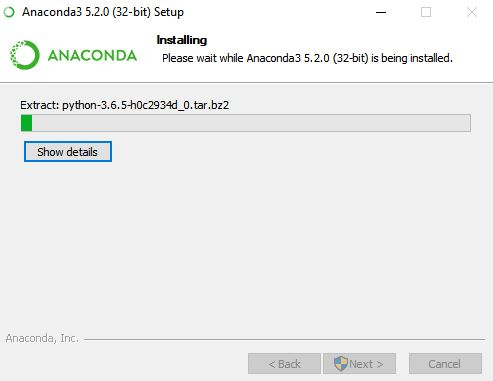
\includegraphics[scale=0.5]{figures/ana1.jpg}
\caption{install anaconda 1}
\label{contoh}
\end{figure}

\par
\item Selanjutnya apabila instalan tersebut telah selesai maka silahkan menekan tombol next
\item Tampilan selanjutnya akan seperti ini

\par

\begin{figure}[ht]
\centering
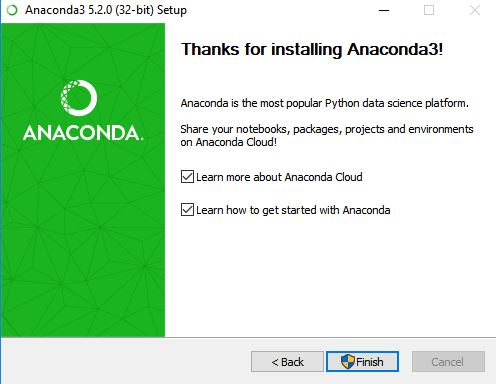
\includegraphics[scale=0.5]{figures/ana2.jpg}
\caption{install anaconda 2}
\label{contoh}
\end{figure}

\par

\item Apabila tampilannya telah sesuai dengan contoh gambar maka instalasi telah selesai
\end{enumerate}
\end{itemize}

\begin{itemize}
\item Instalasi Library Scikit Learn
\begin{enumerate}
\item Silahkan membuka web browser untuk melakukan pengunduhan untuk library scikit dari anaconda.
\item Silahkan mengunjungi halaman ini untuk melakukan pengunduhan library scikit dari anaconda.
\par https://anaconda.org/anaconda/scikit-learn.
\item Setelah terdownload silahkan melakukan instalasi lanjutan menggunakan Command Prompt
\item Silahkan masukkan perintah berikut untuk melakukan pengecekan bahwa anaconda anda telah terpasang dengan baik.
\par conda --version
\par python --version
\item Tampilannya akan nampak seperti berikut :
\par

\begin{figure}[ht]
\centering
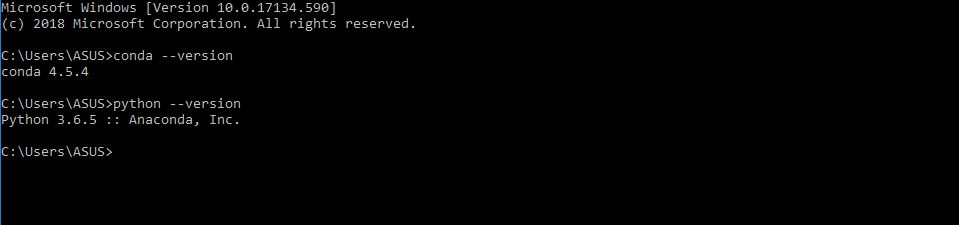
\includegraphics[scale=0.3]{figures/scikit1.jpg}
\caption{Pengecekan Anaconda}
\label{contoh}
\end{figure}

\par
\item Selanjutnya silahkan masukkan perintah berikut untuk melakukan instalasi pip sckit-learn
\par perintahnya : pip install -U scikit-learn
\item Tampilannya akan nampak seperti berikut :
\par

\begin{figure}[ht]
\centering
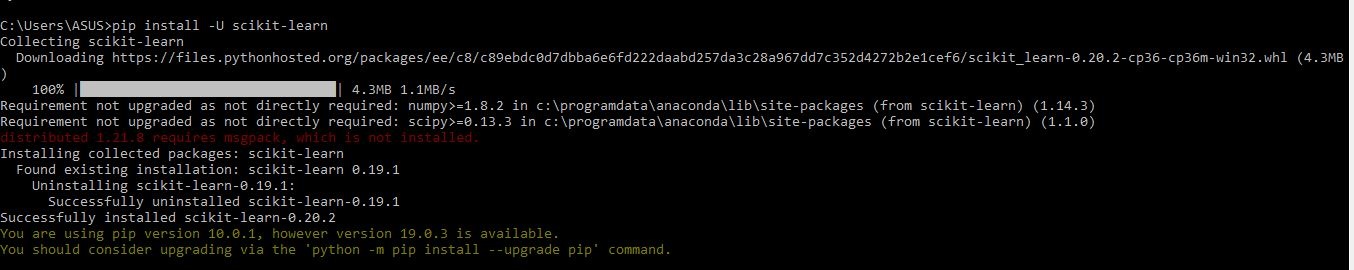
\includegraphics[scale=0.2]{figures/scikit3.jpg}
\caption{instalasi pip scikit-learn}
\label{contoh}
\end{figure}

\par
\item Selanjutnya silahkan masukkan perintah berikut untuk melakukan instalasi conda sckit-learn
\par perintahnya : conda install scikit-learn
\item Tampilannya akan nampak seperti berikut :
\par

\begin{figure}[ht]
\centering
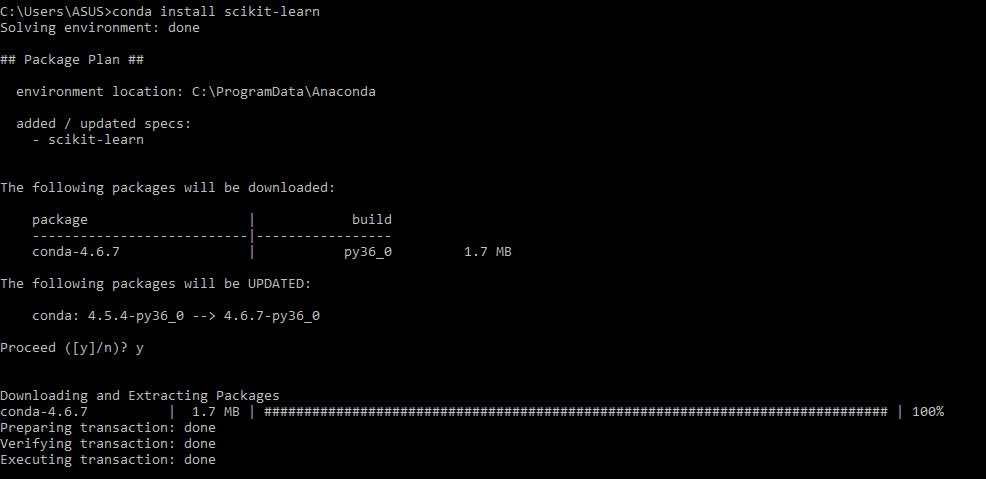
\includegraphics[scale=0.3]{figures/scikit4.jpg}
\caption{instalasi conda scikit-learn}
\label{contoh}
\end{figure}

\par
\par
\par
\item Apabila telah dipraktekan seperti langkah-langkah dan menghasilkan tampilan seperti contoh diatas, maka instalasi scikit-learn dari anaconda berhasil dilakukan
\par
\item Kemudian untuk pengujian yang lain yaitu pengujian untuk mengecek codingan anaconda
\par
\item Contoh uji coba codingannya dapat dilihat pada gambar berikut
\par
\begin{figure}[ht]
\centering
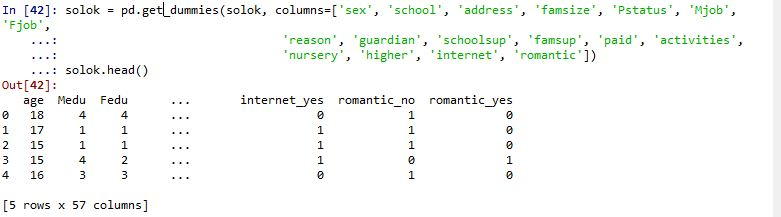
\includegraphics[scale=0.5]{figures/3.jpg}
\caption{uji coba codingan}
\label{contoh}
\end{figure}
\par
\item Berdasarkan pengujian tersebut maka dapat dipastikan bahwa anaconda telah ter-include ke dalam python dan dieksekusi dengan script python
\item Setelah pengeksekusiannya berdasarkan scripts python, terdapatlah keluaran yang sesuai
\item Keluaran tersebut yang menandakan bahwa anacondanya berfungsi dengan baik.
\end{enumerate}
\end{itemize}


\par
\item Loading An Example Dataset
\begin{itemize}
\item Penerapan Loading An Example Dataset Pada Python Di CMD
\begin{enumerate}
\item Pertama-tama silahkan buka command prompt di laptop anda
\item Selanjutnya masuk ke python
\item Setelah masuk kedalam python, silahkan masukkan perintah seperti pada gambar berikut :

\begin{figure}[ht]
\centering
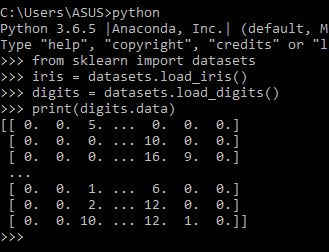
\includegraphics[scale=0.6]{figures/4.jpg}
\caption{pengujian loading an example dataset}
\label{contoh}
\end{figure}

\par
\item Secara keseluruhan, hasilnya pada command prompt akan nampak seperti gambar tersebut
\item Apabila tampilanya telah nampak seperti gambar diatas, maka pengujiannya telah selesai dan berhasil.
\end{enumerate}

\par
\item Penjelasan Perintah Yang Di Uji
\begin{enumerate}
\item Perhatikan perintah yang telah dieksekusi ini :

\par
\begin{figure}[ht]
\centering
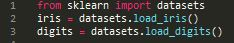
\includegraphics[scale=0.9]{figures/ok4.jpg}
\caption{pengujian loading an example dataset}
\label{contoh}
\end{figure}
\par

\item Penjelasan untuk baris pertama ialah :
\par Perintahnya yaitu memasukkan dan memanggil dataset dari sklearn
\par
\par
\item Penjelasan untuk baris kedua ialah :
\par Terdapat variabel baru yaitu iris. Dimana variabel iris memanggil datasets dan di dalamnya akan ngeload ( menampilkan ) load iris.
\par
\item Penjelasan untuk baris ketiga ialah :
\par Kemudian ada juga variabel baru lainnya yaitu digits yang akan memanggil dataset dan di dalamnya akan ngeload ( menampilkan ) load digits
\par
\item Selanjutnya untuk perintah Print( digits.data ) ditujukan untuk me-
\par nampilkan output dari pengeksekusian variabel digits dan akan berupa data.
\par
\item Hasilnya printnya sebagai berikut :
\par

\begin{figure}[ht]
\centering
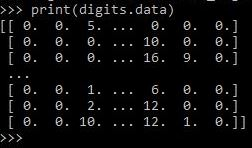
\includegraphics[scale=0.7]{figures/okk4.jpg}
\caption{hasil print uji cobat}
\label{contoh}
\end{figure}

\par
\item Untuk penjelasan uji cobanya sudah selesai.
\par
\end{enumerate}
\end{itemize}
\end{enumerate} 

\section{Teori/Rahmi Roza/1164085}
Teori mencakup resume dari beberapa pembahasan. yaitu :
\begin{itemize}
\item Definisi Kecerdasan Buatan.
\par Kecerdasan Buatan adalah salah satu cabang Ilmu pengetahuan berhubungan dengan pemanfaatan mesin untuk memecahkan persoalan yang rumit dengan cara yang lebih manusiawi. Hal Ini biasanya dilakukan dengan mengikuti/mencontoh karakteristik dan analogi berpikir dari kecerdasan/Inteligensia manusia, dan menerapkannya sebagai algoritma yang dikenal oleh komputer.
\par Agar komputer bisa bertindak seperti dan sebaik manusia, maka komputer juga harus diberi bekal pengetahuan dan mempunyai kemampuan untuk menalar. Untuk itu AI akan mencoba untuk memberikan beberapa metoda untuk membekali komputer dengan kedua komponen tersebut agar komputer bisa menjadi mesin pintar.
\item Sejarah Kecerdasan Buatan
\par Banyak orang percaya kecerdasan buatan akan memusnahkan kelangsungan hidup manusia saat mereka menyadari kekuatan yang dimilikinya. Semua bermula sejak Turing Machine. Berikut perjalanan kecerdasan buatan hingga akhirnya melahirkan robot dan robot seks.
\par Tahun 1950. Alan Turing memperkenalkan Turing Test dalam jurnal berjudul Computering Machinery and Intelligence. Pada musim panas 1956, Konferensi Dartmouth meluncurkan ide artificial intelligence dan IBM memulai riset tentang AI.
\par Tahun 1970. Sepanjang 1974 sampai 1980 merupakan gelombang pertama kecerdasan buatan. Pada periode ini pula pengumpulan dana untuk melakukan riset kecerdasan buatan mulai marak.
\par Tahun 1930. Pada 11 Mei 1997, Deep Blue Computer, kecerdasan buatan besutan IBM berhasil mengalahkan grand master catur asal Rusia, Garry Kasparov
\par Tahun 2000. Kendaraan bikinan tim peneliti dari Universitas Stanford, Amerika Serikat, berhasil menjadi kampiun dal DARPA Grand Challange. Mobil swakemudi ini bisa melaju di gurun pasir sejauh 211 kilometer.
\par Tahun 2010. Watson, kecerdasan buatan besutan IBM, berhasil mengalahkan mantan juara Brad Rutter dan Ken Jennings dalam acara kuis Jeopardy pada pertengahan 2011. Appel, pada 14 Oktober tahun yang sama, memperkenalkan asistem pribadi berbasiskan kecerdasan buatan bernama Siri dalam iPhone 4s. Setahun kemudian, tepatnya Juni, tim dari Google Brain melatih komputer agar bisa mengenali seekor kucing dari jutaan video di YouTube.ChatBot bikinin Eugene Goostman mengklaim telah memecahkan tes Turing dalam kompetisi yang digelar di Universitas Reading, Inggris. Imbasnya, pada Agustus tahun yang sama, banyak ilmuwan mengusulkan untuk membuat tes Turing yang baru. Sementara itu, terkesan dengan kemampuan Watson, NASA menggunakannya untuk penelitian bidang kedirgantaraan.
\par Tahun 2017. Google, Februari lalu, kembali membuat gebrakan soal kecerdasan buatan. Tim dari Google Deep Mind mengungkap kecerdasan buatan memiliki tingkat emosi dan kemarahan yang sama dengan manusia. Kecerdasan buatan pun bisa merasakan kalau dirinya ditipu. Tak mau kalah, Microsoft, April lalu, mendeteksi bahwa artificial intelligence ternyata juga bisa rasis.
Yang paling fenomenal soal kecerdasan buatan pada tahun ini adalah robot seks bernama Harmony. Tak seperti robot seks pada umumnya, Harmony bisa merasakan cemburu dan mendeteksi penggunanya saat hendak menuju klimaks.
\par Jika kita berbicara tentang AI atau Artificial Intelligence maka kita tidak bisa melupakan seorang sosok yang sangat terkenal pada bidang tersebut yaitu bapak John McCarthy.
McCarthy mendapatkan gelar sarjana matematika dari California Institute of Technology (Caltech) pada September 1948. Dari masa kuliahnya itulah ia mulai mengembangkan ketertarikannya pada mesin yang dapat menirukan cara berpikir manusia. McCarthy kemudian melanjutkan pendidikan ke program doktoral di Princeton University.
\par McCarthy kemudian mendirikan dua lembaga penelitian kecerdasan buatan. Kedua lembaga AI itu adalah Stanford Artificial Intelligence Laboratory dan MIT Artificial Inteligence Laboratory. Di lembaga-lembaga inilah bermunculan inovasi pengembangan AI yang meliputi bidang human skill, vision, listening, reasoning dan movement of limbs. Bahkan Salah satu lembaga yang didirikan itu, Stanford Artificial Intelligence pernah mendapat bantuan dana dari Pentagon untuk membuat teknologi-teknologi luar angkasa.

\item Perkembangan Kecerdasan Buatan
\par Perkembangan kecerdasan buatan atau artificial intelligence (AI) dinilai tidak bisa dihentikan. Keberadaan AI justru dinilai akan semakin mempermudah kehidupan manusia dalam beraktivitas. Dalam pandangan Johnny Lie sebagai Vice President of Cheetah Mobile, revolusi teknologi tidak bisa dihentikan. Menurutnya, hal itu sudah terjadi sejak puluhan tahun yang lalu. Cheetah Mobile sendiri merupakan perusahaan teknologi mobile yang fokus pada peranti lunak dan pada hari ini menyematkan unsur AI dalam layanannya.
\par Sebelumnya, beberapa pakar teknologi kenamaan dunia, seperti Elon Musk dan Stephen Hawking gencar memberikan peringatan bahwa AI yamg terus berkembang dapat menjadi ancaman bagi umat manusia. Bahkan, keduanya bersama banyak ilmuwan lainnya membuat surat penegasan kepada PBB untuk mengawasi pertumbuhan AI.
\par Dengan AI, sebuah produk teknologi dapat bekerja lebih cerdas dan mandiri. Misalnya saja, sebuah aplikasi smartphone yang menggunakan AI dapat mempelajari kebiasaan pengguna. Alhasil, Anda tidak perlu repot lagi dalam melakukan suatu pekerjaan di ponsel.
\end{itemize}
\item Tentang Pengertian Terhadap Ilmu Yang Lain
\begin{itemize}
\item Supervised learning adalah sebuah pendekatan dimana sudah terdapat data yang dilatih, dan terdapat variable yang ditargetkan sehingga tujuan dari pendekatan ini adalah mengkelompokan suatu data ke data yang sudah ada
\par
\item Klasifikasi adalah pembagian sesuatu menurut kelas-kelas ( class ). Menurut Ilmu Pengetahuan, Klasifikasi merupakan proses pengelompokkan benda berdasarkan ciri-ciri persamaan dan juga perbedaan.
\par
\item Regresi adalah metode analisis statistik yang digunakan untuk melihat pengaruh antara dua ataupun lebih variabel.
\par
\item Unsupervised Learning berbeda dengan Supervised Leraning. Perbedaannya ialah unsupervised learning tidak memiliki data latih, sehingga dari data yang ada kita mengelompokan data tersebut menjadi 2  ataupun 3 bagian dan seterusnya.
\par
\item Dataset adalah objek yang merepresentasikan data dan juga relasi yang ada di memory.
\par
\item Training Set adalah set digunakan oleh algoritma klassifikasi . Dapat dicontohkan dengan :  decision tree, bayesian, neural network dll. Semuanya dapat digunakan untuk membentuk sebuah model classifier.
\par
\item Testing Set adalah set yang digunakan untuk mengukur sejauh mana classifier berhasil melakukan klasifikasi dengan benar.
\par
\end{itemize}
\end{enumerate}

\chapter{Related Works}

Your related works, and your purpose and contribution which must be different as below.

\section{Fadila/1164072}
\subsection{Teori}
Penyelesaian Tugas Harian 3 ( No. 1-7 )
\begin{enumerate}
\item Binary Classification Dan Ilustrasi Gambarnya
\begin{itemize}
\item Pengertian Binary Classification / Klasifikasi Biner:
\par Klasifikasi biner atau binomial merupakan tugas untuk mengklasifikasikan elemen-elemen dari himpunan tertentu ke dalam dua kelompok (memprediksi kelompok mana yang masing-masing dimiliki) ber-
\par dasarkan aturan klasifikasi.
\item Ilustrasi Gambar Binary Classification :
\par

\begin{figure}[ht]
\centering
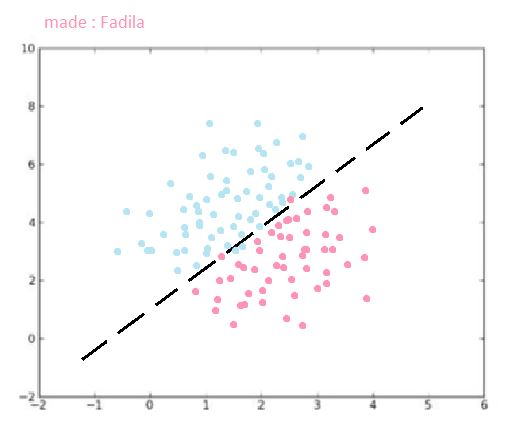
\includegraphics[scale=0.3]{figures/binary.jpg}
\caption{binary classification}
\label{contoh}
\end{figure}

\par
\end{itemize}
\item Supervised Learning, Unsupervised Learning, Clustering Dan Ilustrasi Gambar
\begin{itemize}
\item Pengertian Supervised Learning :
\par Sebuah pendekatan dimana terdapat data yang dilatih dan ditargetkan. Leih singkatnya supervised learning memiliki kategori sehingga tujuan dan outputnya jelas.
\begin{itemize}
\par
\item Ilustrasi Gambar Supervised Learning :

\begin{figure}[ht]
\centering
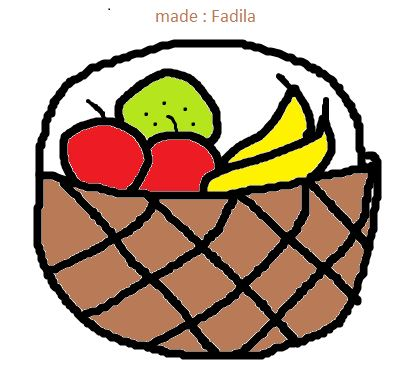
\includegraphics[scale=0.4]{figures/supervised1.jpg}
\caption{supervised}
\label{contoh}
\end{figure}


\par Pada contoh gambar diatas dikelompokkan bahwa apabila bentuk dari objek di gambar berbentuk bundar dan berwarna merah maka akan dinamakan atau di sebut sebagai Apel. Dan apabila pada gambar terdapat objek berbentuk panjang dan berwarna kuning maka akan dinamakan atau di sebut sebagai pisang.
\par
\end{itemize}

\par
\item Pengertian Unsupervised Learning :
\par Tidak memiliki data latih, sehingga dari data yang tersebut kita bisa mengelompokkannya ke berbagai kelompok 2 seterusnya. Dengan lebih singkatnya ialah unsupervised learning tidak memiliki kategori.
\par
\par
\begin{itemize}
\item Ilustrasi Gambar Unsupervised Learning :

\begin{figure}[ht]
\centering
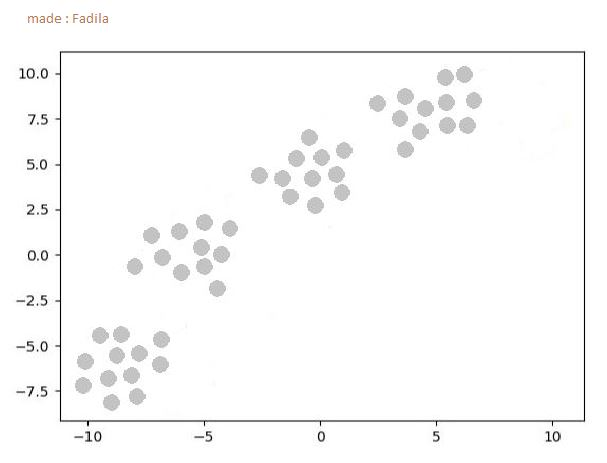
\includegraphics[scale=0.4]{figures/unsupervised2.jpg}
\caption{unsupervised}
\label{contoh}
\end{figure}

\par Pada gambar dapat dilihat bahwa ada banyak data namun tidak pada pengelompokkan yang tepat. Cuman dapat dikelompokkan ke dalam berbagai macam bentuk dan jumlah namun tidak memberikan output yang jelas.
\par
\par
\end{itemize}
\item Pengertian Clustering :
\par Metode pengelompokan data. Clustering juga merupakan proses partisi satu set objek data ke dalam himpunan bagian yang disebut dengan cluster. Objek dalam cluster tersebut memiliki kemiripan karakteristik antar satu sama lain.
\par

\begin{figure}[ht]
\centering
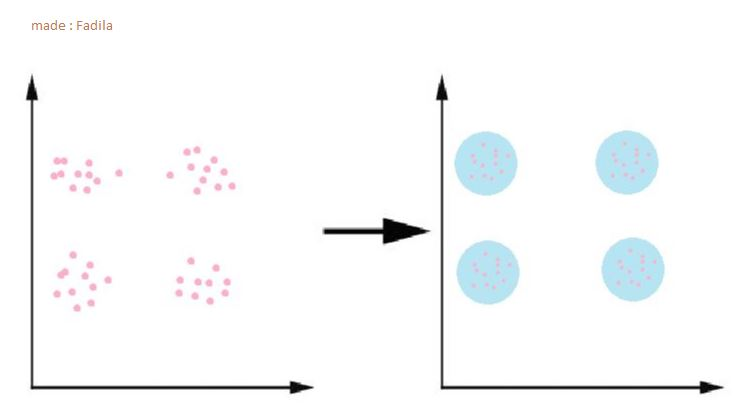
\includegraphics[scale=0.5]{figures/clustering.jpg}
\caption{clustering}
\label{contoh}
\end{figure}

\par
\end{itemize}
\item Evaluasi, Akurasi Dan Ilustrasi Gambar
\begin{itemize}
\item Pengertian Evaluasi
\par Evaluasi digunakan untuk memeriksa/memastikan dan mengevaluasi model dalam bekerja ( seberapa baik ) dengan mengukur keakuratannya. Kita juga dapat menanalisis kesalahan yang dibuat pada model yang dijalankan, tingkat kebingungan dan menggunakan matriks kebingunan.
\par

\begin{figure}[ht]
\centering
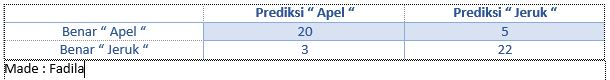
\includegraphics[scale=0.6]{figures/eva.jpg}
\caption{Evaluasi}
\label{contoh}
\end{figure}

\par Pada contoh gambar dapat dilihat bahwa dilakukan evaluasi terhadap kerja dalam penentuan jenis dari objek. Dievaluasi berapa banyak sebuah objek ketika dikelompokkan dan diklasifikasikan kemudian dapat dilihat apakah kerjanya sesuai atau tidak.
\par

\par
\item Pengertian Akurasi
\par Accuracy akan didefinisikan sebagai presentasi kasus yang diklasifikasikan dengan benar. Accuracy lebih jelasnya adalah perbandingan kasus yang diidentifikasi benar dengan jumlah semua kasus
 \par Rumus dari accuracy= (a+c)/(a+b+c+d)
\par

\begin{figure}[ht]
\centering
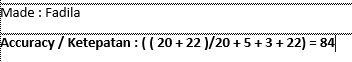
\includegraphics[scale=0.8]{figures/acuracy.jpg}
\caption{Akurasi}
\label{contoh}
\end{figure}

\par Dilakukan perhitungan dengan rumus akurasi terhadap data yang telah diolah pada " Evaluasi ". Kemudian di dapatkan hasil dari pengolahan data tersebut.
\par Contoh penggabungan Akurasi Dan Evaluasi
\par

\begin{figure}[ht]
\centering
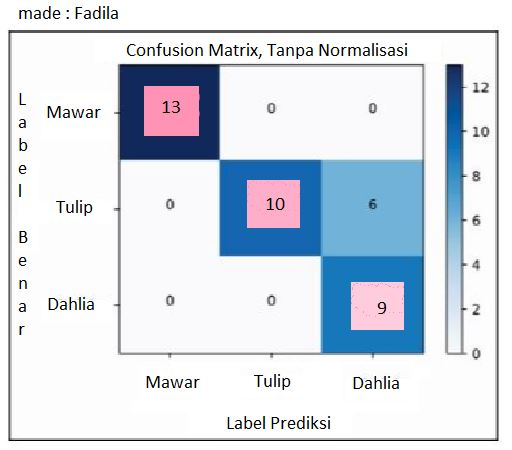
\includegraphics[scale=0.5]{figures/evacuray.jpg}
\caption{Contoh Evaluasi Dan Akurasi Secara Bersamaan }
\label{contoh}
\end{figure}

\end{itemize}

\par
\item Membuat Dan Membaca Confusion Matrix Beserta Contoh
\begin{itemize}
\item Pengertian Confusion Matrix
\par Confusion matrix merupakan suatu metode yang  digunakan untuk melakukan perhitungan akurasi pada konsep data mining.
\par
\item Pembacaan Confusion Matrix
\begin{enumerate}
\item Apabila hasil prediksi negatif dan data sebenarnya merupakan negatif.
\item Apabila hasil prediksi positif sedangkan nilai sebenarnya merupakan negatif.
\item Apabila hasil prediksi negatif sedangkan nilai sebenarnya merupakan positif.
\item Apabila hasil prediksi positif dan nilai sebenarnya merupakan positif.
\end{enumerate}
\par
\par
\item Pembuatan Confusion Matrix
\begin{enumerate}
\item Menentukan 4 proses klasifikasi yang akan digunakan dalam confusion matrix.
\item 4 Istilah tersebut ada True Positive ( TP ), True Negative ( TN ), False Positive ( FP ) dan False Negative ( FN ).
\item Kelompokkan klasifikasi tersebut bisa menggunakan klasifikasi biner
\item Akan menghasilkan keluaran berupa 2 Kelas ( Positif dan Negatif ) dan penentuan TP, FP ( 1 klasifikasi positif ) , FN dan TN ( 1 klasifikasi negatif ).
\item Contoh dasarnya nampak seperti langkah diatas
\item Istilahnya daat didefinisikan dengan objek lain namu dengan alur yang sama ( sesuai rumus baik klasifikasi dll ).
\end{enumerate}
\par

\item Ilustrasi Gambar
\par

\begin{figure}[ht]
\centering
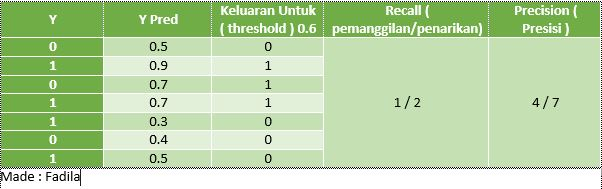
\includegraphics[scale=0.6]{figures/confusion.jpg}
\caption{confusion matrix}
\label{contoh}
\end{figure}

\par
\begin{itemize}
\item Penjelasan
\begin{enumerate}
\item Recall
\par Dari semua kelas positif, seberapa banyak yang kami prediksi dengan benar. Itu harus setinggi mungkin.
\par

\begin{figure}[ht]
\centering
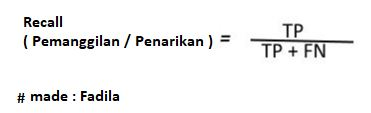
\includegraphics[scale=0.6]{figures/recall.jpg}
\caption{recall}
\label{contoh}
\end{figure}

\par
\item Presisi / Precision
\par Dari semua kelas, seberapa banyak yang kami prediksi dengan benar. Itu harus setinggi mungkin.
\par

\begin{figure}[ht]
\centering
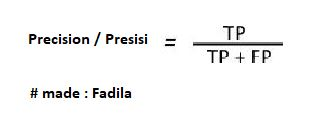
\includegraphics[scale=0.6]{figures/precision.jpg}
\caption{precision}
\label{contoh}
\end{figure}

\par
\item F-Ukur ( measure )
\par Sulit untuk membandingkan dua model dengan presisi rendah dan daya ingat tinggi atau sebaliknya. Jadi untuk membuatnya sebanding, kami menggunakan F-Score. F-score membantu mengukur Recall dan Precision pada saat yang bersamaan
\par

\begin{figure}[ht]
\centering
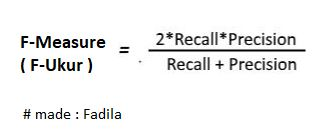
\includegraphics[scale=0.6]{figures/f.jpg}
\caption{f-measure}
\label{contoh}
\end{figure}

\par
\end{enumerate}
\end{itemize}
\end{itemize}


\par
\item Cara Kerja K-Fold Classification Dan Ilustrasi Gambar
\begin{enumerate}
\item Pertama-tama untuk total instance dibagi menjadi N bagian.
\item Fold ke-1 ( atau pertama ) adalah ketika bagian ke-1 menjadi data uji (testing data) dan sisanya menjadi data latih (training data).
\item Hitung akurasi ( berdasarkan porsi data tersebut. Persamaanya sebagai berikut :
\par (sigma) data klasifikasi
\par (sigma) total data uji
\par x 100 persen 
\item Fold ke-2 ( kedua ) adalah ketika bagian ke-2 menjadi data uji (testing data) dan sisanya menjadi data latih (training data). 
\item Kemudian dihitunglah akurasi berdasarkan porsi data yang telah ditentukan
\item Demikian seterusnya hingga mencapai fold ke-K. Hitung rata-rata akurasi dari K buah akurasi di atas. Rata-rata akurasi ini menjadi akurasi final atau akhir.
\end{enumerate}
\par
\begin{itemize}
\item Ilustrasi Gambar
\par

\begin{figure}[ht]
\centering
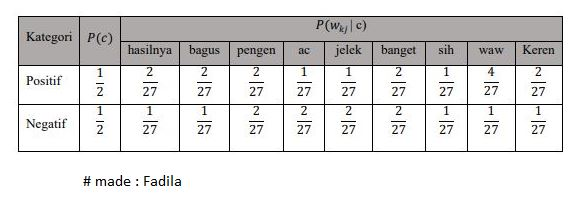
\includegraphics[scale=0.4]{figures/hasilk1.jpg}
\caption{k-fold classification 1}
\label{contoh}
\end{figure}

\begin{figure}[ht]
\centering
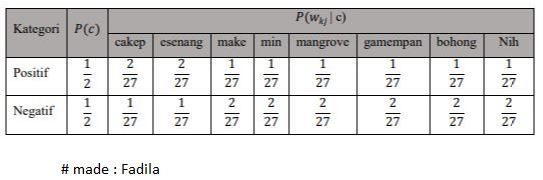
\includegraphics[scale=0.4]{figures/hasilk2.jpg}
\caption{k-fold classification 2}
\label{contoh}
\end{figure}

\par
\par
\end{itemize}

\par
\item Decision Tree Dan Ilustrasi Gambar
\begin{itemize}
\item Pengertian Decision Tree
\par Decision tree adalah salah satu metode klasifikasi yang paling populer karena mudah diinterpretasikan oleh manusia. Decision tree merupakan metode klasifikasi yang digunakan untuk pengenalan pola dan termasuk dalam pengenalan pola secara statistik. 3 tipe dari decision tree ialah:  simpul: simpul root, simpul perantara, dan simpul leaf.
\par

\end{itemize}
\par

\par
\begin{itemize}
\item Ilustrasi Gambar
\par


\begin{figure}[ht]
\centering
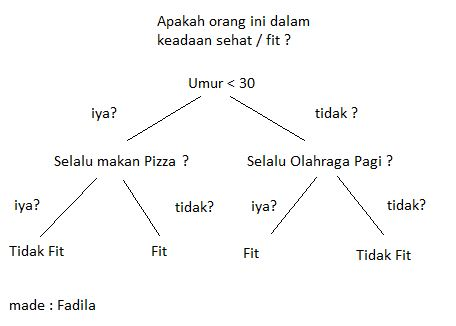
\includegraphics[scale=0.5]{figures/decisiontree.jpg}
\caption{decision tree}
\label{contoh}
\end{figure}

\par
\end{itemize}
\item Information Gain Dan Entropi
\begin{itemize}
\item Pengertian Information Gain
\par Information Gain adalah salah satu atribute selection measure yang digunakan untuk memilih test atribute tiap node pada tree.
\par Algoritme Information Gain digunakan untuk mengurangi dimensi atribut untuk mendapatkan atribut-atribut yang relevan. 
\par

\begin{itemize}
\item Ilustrasi Gambar
\par


\begin{figure}[ht]
\centering
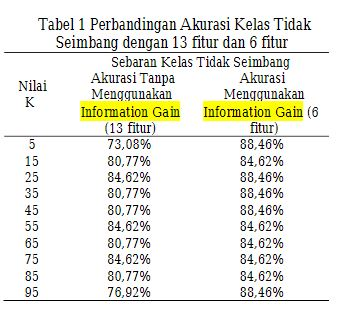
\includegraphics[scale=0.6]{figures/information1.jpg}
\caption{informaion gain 1}
\label{contoh}
\end{figure}


\begin{figure}[ht]
\centering
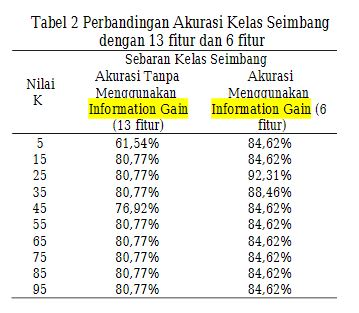
\includegraphics[scale=0.6]{figures/information2.jpg}
\caption{information gain 2}
\label{contoh}
\end{figure}

\item Penjelasan :
\par Tabel  1  sampai  dengan  Tabel  2 menunjukkan  bahwa  penggunaan  seleksi fitur Information  Gain  menghasilkan  nilai  akurasi yang  lebih  baik  dibandingkan  tanpa menggunakan Information Gain. 
\par Pada saat nilai K sama dengan 5 ( K=5) akurasi  yang  dihasilkan  sistem  tanpa menggunakan  Information  Gain  menunjukkan hasil  yang  kurang  baik  pada  sebaran  kelas seimbang maupun tak seimbang yaitu  61,54 persen pada sebaran kelas seimbang dan 73,08 persen pada sebaran  kelas tidak  seimbang. 
\end{itemize}


\par
\item Pengertian Entropi
\par Entropi pada umumnya merupakan salah satu besaran yang mengukur energi dalam sistem per satuan temperatur yang tak dapat digunakan untuk melakukan usaha.
\par Namun, secara spesifik untuk " Entropi " sendiri merupakan parameter untuk mengukur tingkat keberagaman (heterogenitas) dari kumpulan data. 

\par

\begin{figure}[ht]
\centering
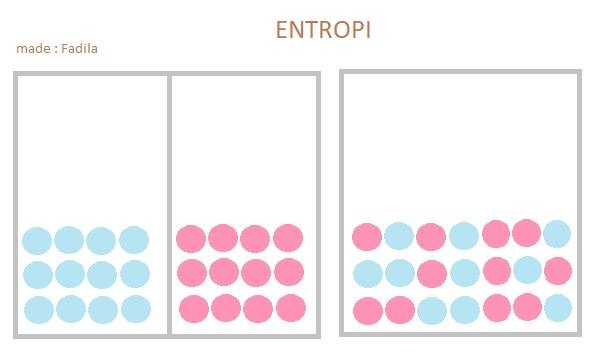
\includegraphics[scale=0.5]{figures/entropi.jpg}
\caption{entropi}
\label{contoh}
\end{figure}

\par
\end{itemize}

\end{enumerate}

\section{Lusia Violita Aprilian/1164080}
\subsection{binary classification dilengkapi ilustrasi gambar}
\begin{enumerate}
\item Binary classification yaitu berupa kelas positif dan kelas negatif. Klasifikasi biner adalah dikotomisasi yang diterapkan untuk tujuan praktis, dan dalam banyak masalah klasifikasi biner praktis, kedua kelompok tidak simetris - daripada akurasi keseluruhan, proporsi relatif dari berbagai jenis kesalahan yang menarik. Misalnya, dalam pengujian medis, false positive (mendeteksi penyakit ketika tidak ada) dianggap berbeda dari false negative (tidak mendeteksi penyakit ketika hadir).
\begin{figure}[ht]
\centering
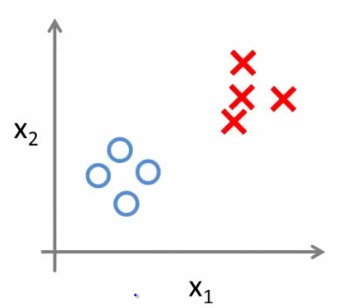
\includegraphics[scale=0.5]{figures/f1.jpg}
\caption{Binary Classification}
\label{contoh}
\end{figure}

\subsection{supervised learning dan unsupervised learning dan clustering
dengan ilustrasi gambar}
\item Supervised learning adalah tugas pembelajaran mesin untuk mempelajari suatu fungsi yang memetakan input ke output berdasarkan contoh pasangan input-output. Ini menyimpulkan fungsi dari data pelatihan berlabel yang terdiri dari serangkaian contoh pelatihan. Dalam pembelajaran yang diawasi, setiap contoh adalah pasangan yang terdiri dari objek input (biasanya vektor) dan nilai output yang diinginkan (juga disebut sinyal pengawas). Algoritma pembelajaran yang diawasi menganalisis data pelatihan dan menghasilkan fungsi yang disimpulkan, yang dapat digunakan untuk memetakan contoh-contoh baru. Skenario optimal akan memungkinkan algoritma menentukan label kelas dengan benar untuk instance yang tidak terlihat. Ini membutuhkan algoritma pembelajaran untuk menggeneralisasi dari data pelatihan untuk situasi yang tidak terlihat dengan cara yang "masuk akal" (lihat bias induktif). Tugas paralel dalam psikologi manusia dan hewan sering disebut sebagai pembelajaran konsep.
\begin{figure}[ht]
\centering
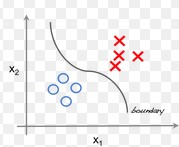
\includegraphics[scale=0.5]{figures/f2.jpg}
\caption{Supervised Learning}
\label{contoh}
\end{figure}
\item Unsupervised learning adalah istilah yang digunakan untuk pembelajaran bahasa Ibrani, yang terkait dengan pembelajaran tanpa guru, juga dikenal sebagai organisasi mandiri dan metode pemodelan kepadatan probabilitas input. Analisis cluster sebagai cabang pembelajaran mesin yang mengelompokkan data yang belum diberi label, diklasifikasikan atau dikategorikan. Alih-alih menanggapi umpan balik, analisis klaster mengidentifikasi kesamaan dalam data dan bereaksi berdasarkan ada tidaknya kesamaan di setiap potongan data baru.
\begin{figure}[ht]
\centering
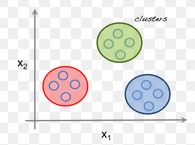
\includegraphics[scale=0.5]{figures/f3.jpg}
\caption{Unsupervised Learning}
\label{contoh}
\end{figure}
\item Cluster analysis or clustering adalah tugas pengelompokan sekumpulan objek sedemikian rupa sehingga objek dalam kelompok yang sama (disebut klaster) lebih mirip (dalam beberapa hal) satu sama lain daripada pada kelompok lain (kluster). Ini adalah tugas utama penambangan data eksplorasi, dan teknik umum untuk analisis data statistik, yang digunakan di banyak bidang, termasuk pembelajaran mesin, pengenalan pola, analisis gambar, pengambilan informasi, bioinformatika, kompresi data, dan grafik komputer. Analisis Cluster sendiri bukan merupakan salah satu algoritma spesifik, tetapi tugas umum yang harus dipecahkan. Ini dapat dicapai dengan berbagai algoritma yang berbeda secara signifikan dalam pemahaman mereka tentang apa yang merupakan sebuah cluster dan bagaimana cara menemukannya secara efisien. Gagasan populer mengenai cluster termasuk kelompok dengan jarak kecil antara anggota cluster, area padat ruang data, interval atau distribusi statistik tertentu. Clustering karena itu dapat dirumuskan sebagai masalah optimasi multi-objektif. Algoritma pengelompokan dan pengaturan parameter yang sesuai (termasuk parameter seperti fungsi jarak yang akan digunakan, ambang kepadatan atau jumlah cluster yang diharapkan) tergantung pada set data individual dan penggunaan hasil yang dimaksudkan. Analisis kluster bukan merupakan tugas otomatis, tetapi proses berulang penemuan pengetahuan atau optimasi multi-objektif interaktif yang melibatkan percobaan dan kegagalan. Seringkali diperlukan untuk memodifikasi praproses data dan parameter model hingga hasilnya mencapai properti yang diinginkan.
\begin{figure}[ht]
\centering
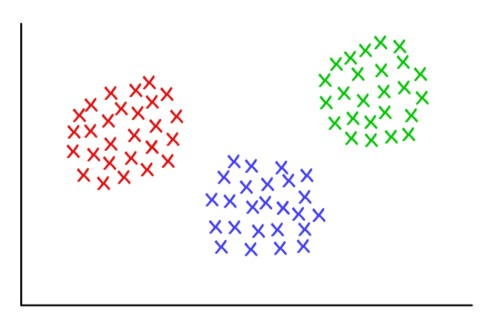
\includegraphics[scale=0.5]{figures/f4.jpg}
\caption{Cluster}
\label{contoh}
\end{figure}

\subsection{evaluasi dan akurasi dari buku dan disertai ilustrasi contoh
dengan gambar}
\begin{enumerate}
\item Evaluasi adalah tentang  bagaimana kita dapat mengevaluasi seberapa baik model bekerja dengan mengukur akurasinya. Dan akurasi akan didefinisikan sebagai persentase kasus yang diklasifikasikan dengan benar. Kita dapat menganalisis kesalahan yang dibuat oleh model, atau tingkat kebingungannya, menggunakan matriks kebingungan. Matriks kebingungan mengacu pada kebingungan dalam model, tetapi matriks kebingungan ini bisa menjadi sedikit sulit untuk dipahami ketika mereka menjadi sangat besar.
\begin{figure}[ht]
\centering
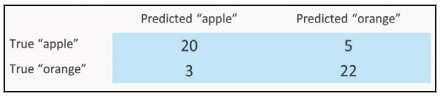
\includegraphics[scale=0.5]{figures/f9.jpg}
\caption{ Evaluasi dan Akurasi}
\label{contoh}
\end{figure}

\subsection{ bagaimana cara membuat dan membaca confusion matrix, buat confusion matrix }
\begin{enumerate}
\item Cara membuat dan membaca confusion matrix :
\begin{itemize}
\item 1)	Tentukan pokok permasalahan dan atributanya, misal gaji dan listik.
\item 2)	Buat pohon keputusan
\item 3)	Lalu data testingnya
\item 4)	Lalu mencari nilai a, b, c, dan d. Semisal a = 5, b = 1, c = 1, dan d = 3.
\item 5)	Selanjutnya mencari nilai recall, precision, accuracy, serta dan error rate.
\end{itemize}
\item Berikut adalah contoh dari confusion matrix :
\begin{itemize}
\item Recall =3/(1+3) = 0,75
\item Precision = 3/(1+3) = 0,75
\item Accuracy =(5+3)/(5+1+1+3) = 0,8
\item Error Rate =(1+1)/(5+1+1+3) = 0,2
\end{itemize}

\subsection{bagaimana K-fold cross validation bekerja dengan gambar ilustrasi}
\begin{enumerate}
\item Cara kerja K-fold cross validation :
\begin{itemize}
\item 1)	Total instance dibagi menjadi N bagian.
\item 2)	Fold yang pertama adalah bagian pertama menjadi data uji (testing data) dan sisanya menjadi training data.
\item 3)	Lalu hitung akurasi berdasarkan porsi data tersebut dengan menggunakan persamaan.
\item 4)	Fold yang ke dua adalah bagian ke dua menjadi data uji (testing data) dan sisanya training data. 
\item 5)	Kemudian hitung akurasi berdasarkan porsi data tersebut.
\item 6)	Dan seterusnya hingga habis mencapai fold ke-K.
\item 7)	Terakhir hitung rata-rata akurasi K buah.
\end{itemize}
\begin{figure}[ht]
\centering
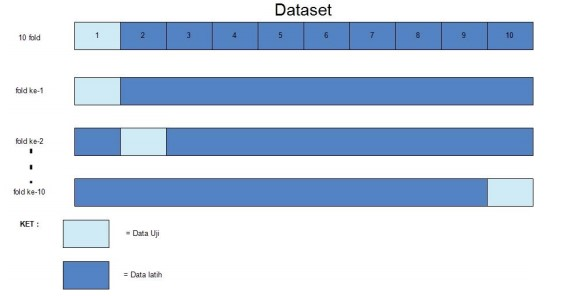
\includegraphics[scale=0.5]{figures/f5.jpg}
\caption{K-fold cross validation }
\label{contoh}
\end{figure}

\subsection{decision tree dengan gambar ilustrasi}
\begin{enumerate}
\item Decision tree adalah model visual yang terdiri dari node dan cabang, seperti Gambar dijelaskan secara rinci nanti dalam artikel ini. Untuk saat ini, amati bahwa ia tumbuh dari kiri ke kanan, dimulai dengan simpul keputusan root (kuadrat, juga disebut simpul pilihan) yang cabang-cabangnya mewakili dua atau lebih opsi bersaing yang tersedia bagi para pembuat keputusan. Pada akhir cabang awal ini, ada simpul akhir (segitiga, juga disebut simpul nilai) atau simpul ketidakpastian (lingkaran, juga disebut simpul peluang). Node akhir mewakili nilai tetap. Cabang lingkaran mewakili hasil yang mungkin bersama dengan probabilitasnya masing-masing (yang berjumlah 1,0). Di luar cabang-cabang node ketidakpastian awal ini, mungkin ada lebih banyak bujur sangkar dan lebih banyak lingkaran, yang umumnya bergantian sampai setiap jalur berakhir di simpul akhir.
\begin{figure}[ht]
\centering
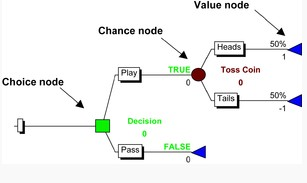
\includegraphics[scale=0.5]{figures/f6.jpg}
\caption{Decision Tree}
\label{contoh}
\end{figure}

\subsection{Information gain dan entropi dengan gambar ilustrasi}
\begin{enumerate}
\item Information gain (IG) mengukur seberapa banyak "informasi" fitur memberi kita tentang kelas. - Fitur yang sempurna mempartisi harus memberikan informasi maksimal. - Fitur yang tidak terkait seharusnya tidak memberikan informasi.
\begin{figure}[ht]
\centering
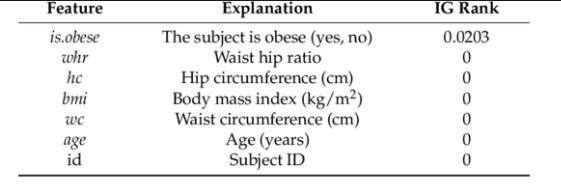
\includegraphics[scale=0.5]{figures/f7.jpg}
\caption{Information gain}
\label{contoh}
\end{figure}
\begin{enumerate}
\item Entropi merupakan kemurnian dalam koleksi contoh yang sewenang-wenang.
\begin{figure}[ht]
\centering
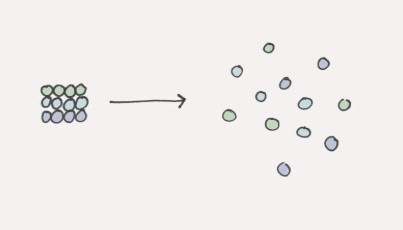
\includegraphics[scale=0.5]{figures/f8.jpg}
\caption{Entropi}
\label{contoh}
\end{figure} 
\chapter{Methods}

\section{The data}
PLease tell where is the data come from, a little brief of company can be put here.

\section{Method 1}
Definition, steps, algoritm or equation of method 1 and how to apply into your data
\section{Method 2}
Definition, steps, algoritm or equation of method 2 and how to apply into your data
\chapter{Klasifikasi Teks}
brief of experiment and result.

\section{Lusia Violita Aprilian/1164080}

\subsection{Teori}
\begin{enumerate}
\item Klasifikasi teks
	\par Klasifikasi Dokumen / Teks adalah salah satu tugas penting dan tipikal dalam supervised machine learning (ML). Menetapkan kategori pada dokumen, yang dapat berupa halaman web, buku perpustakaan, artikel media, galeri, dll. Memiliki banyak aplikasi seperti mis. penyaringan spam, perutean email, analisis sentimen dll. 
	\begin{figure}[ht]
		\centering
		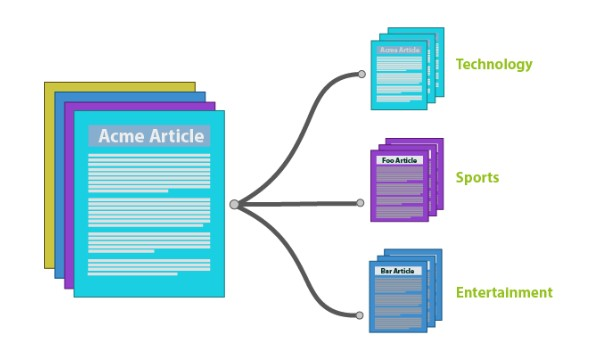
\includegraphics[scale=0.5]{figures/m1.jpg}
		\caption{Lusia-Klasifikasi teks}
		\label{contoh}
	\end{figure}
	
\item Klasifikasi Bunga tidak dapat penggunakan machine learning
	\par Klasifikasi bunga tidak dapat menggunakan machine learning karena memiliki masalah input yang serupa namun output yang berbeda atau 'noise'. Yang dimaksud dengan noise adalah contoh output yang direkam bukan seperti seharusnya. Misalnya saja kita secara implisit berasumsi bahwa contoh bunga kita telah diklasifikasikan dengan benar. Tetapi ini harus dilakukan dengan seseorang yang tepat, seperti seorang ahli botani. Seorang ahli botani ahli harus melihat contoh bunga dan berkata: " ini adalah setosa ... ini adalah virginica ", dan dengan demikian bertindak sebagai "guru" yang memungkinkan mesin untuk belajar. Tetapi bagaimana jika guru itu melakukan kesalahan? Selain itu, selalu ada peluang untuk memperkenalkan kesalahan saat merekam data. Noise juga ditemukan dalam pengukuran, yang selalu sedikit bermasalah karena alat dan sensor kami tidak sempurna dan hanya bekerja pada tingkat presisi tertentu.
	\begin{figure}[ht]
		\centering
		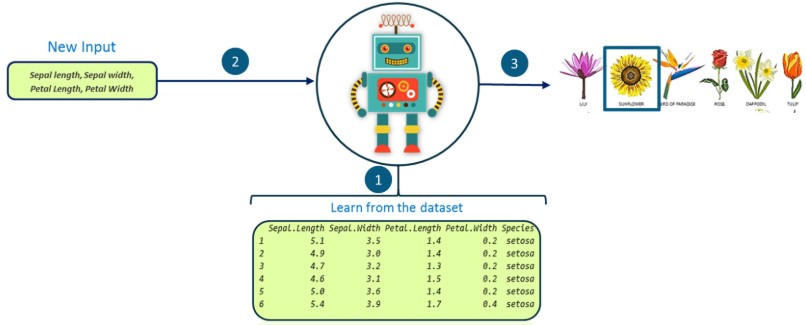
\includegraphics[scale=0.5]{figures/m2.jpg}
		\caption{Lusia-Klasifikasi bunga}
		\label{contoh}
	\end{figure}

\item Teknik pembelajaran mesin pada teks YouTube
	\par Dengan menggunakan kasus seperti rekomendasi video yang terdapat pada fiturnya, Machine Learning pada YouTube memperhatikan apa saja yang menarik perhatian para penggunanya. Ketika kita sedang menonton di YouTube, pada sebelah kanan terdapat 'Up Next' yang menampilkan beberapa video serupa yang sedang ditonton. Dan ketika mengklik salah satu video dari baris tersebut, maka YouTube akan mengingatnya dan menggunakan kata yang tertera sebagai referensi. 
	\begin{figure}[ht]
		\centering
		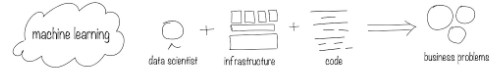
\includegraphics[scale=0.5]{figures/m3.jpg}
		\caption{Lusia-Teknik YouTube}
		\label{contoh}
	\end{figure}

\item Vectorisasi Data
	\begin{itemize}
		\item Maksud dari Vectorisasi Data merupakan Pemecahan dan Pembagian Data.
	\end{itemize}
	
\item Bag of word
	\par Bag-of-words adalah cara untuk merepresentasikan data teks saat memodelkan teks dengan algoritma pembelajaran mesin.
	\begin{figure}[ht]
		\centering
		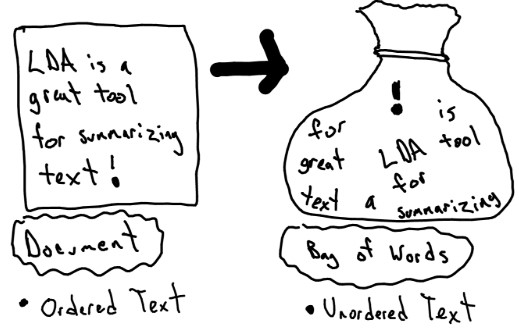
\includegraphics[scale=0.5]{figures/m5.jpg}
		\caption{Lusia-Bag of Word}
		\label{contoh}
	\end{figure}
	
\item TF-IDF
	\par TF-IDF merupakan istilah frekuensi - frekuensi dokumen terbalik, adalah ukuran penilaian yang banyak digunakan dalam pengambilan informasi (IR) atau peringkasan. TF-IDF dimaksudkan untuk mencerminkan seberapa relevan suatu istilah dalam dokumen yang diberikan. Intuisi di baliknya adalah bahwa jika sebuah kata muncul beberapa kali dalam sebuah dokumen, kita harus meningkatkan relevansinya karena itu harus lebih bermakna daripada kata-kata lain yang muncul lebih sedikit kali (TF). Pada saat yang sama, jika sebuah kata muncul berkali-kali dalam suatu dokumen tetapi juga di sepanjang banyak dokumen lain, mungkin itu karena kata ini hanya kata yang sering; bukan karena itu relevan atau bermakna (IDF).
	\begin{figure}[ht]
		\centering
		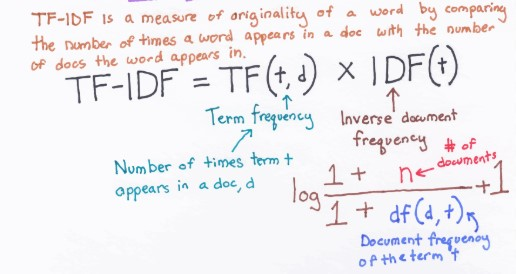
\includegraphics[scale=0.5]{figures/m6.jpg}
		\caption{Lusia-TF IDF}
		\label{contoh}
	\end{figure}
\end{enumerate}

\subsection{Praktek}
\begin{enumerate}
\item Aplikasi menggunakan pandas
	\par Berikut adalah aplikasi yang dibuat menggunakan pandas :
	
		\begin{figure}[ht]
		\centering
		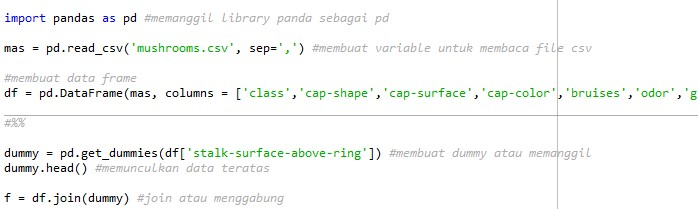
\includegraphics[scale=0.5]{figures/n1a.jpg}
		\caption{Lusia-Pandas}
		\label{contoh}
		\end{figure}
		
	\begin{enumerate}
	\item 1 = memanggil library pandas sebagai pd
	\item 2 = membuat varible mas untuk membaca foile csv
	\item 3 = membuat varible untuk membuat data frame
	\item 4 = membuat variable dummy untuk mengubah kategori menjadi integer
	\item 5 = untuk memunculkan data teratas
	\item 6 = untuk menjoinkan atau menggabungkan data frame dengan dummy
	\end{enumerate}
	
	\par Berikut adalah hasilnya :
	
		\begin{figure}[ht]
		\centering
		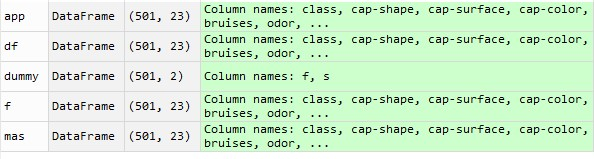
\includegraphics[scale=0.5]{figures/n1b.jpg}
		\caption{Lusia-Hasil Pandas}
		\label{contoh}
		\end{figure}	
	
\item Memecah data frame
	\par Berikut untuk memecah data frame menjadi dua :
	
		\begin{figure}[ht]
		\centering
		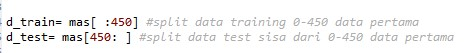
\includegraphics[scale=0.5]{figures/n2a.jpg}
		\caption{Lusia-Pecah data}
		\label{contoh}
		\end{figure}
	
	\begin{enumerate}
	\item 1 = split data training 0-450 data pertama
	\item 2 = split data test sisa dari 0-450 data pertama
	\end{enumerate}
	
	\par Berikut adalah hasilnya :
	
		\begin{figure}[ht]
		\centering
		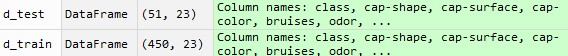
\includegraphics[scale=0.5]{figures/n2b.jpg}
		\caption{Lusia-Hasil Pecah data}
		\label{contoh}
		\end{figure}
		
\item Vektorisasi dan klasifikasi Decission Tree Katty Perry
	\begin{itemize}
	\item Berikut adalah vektorisasi dan klasifikasi Katty Perry
		\begin{figure}[ht]
		\centering
		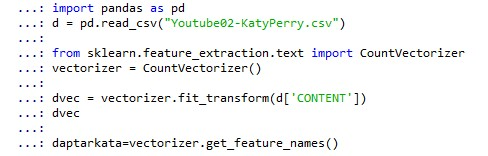
\includegraphics[scale=0.5]{figures/n3a.jpg}
		\caption{Lusia-Vektorisasi dan klasifikasi}
		\label{contoh}
		\end{figure}
	\par Maksud dari gambar vektorisasi dan klasifikasi Katty Perry adalah hasil dari impor dataset, lalu import countvectorizer dari sklearn. Modul sklearn feature extraction digunakan untuk mengekstrak fitur dalam format yang didukung oleh algoritma pembelajaran mesin dari kumpulan data yang terdiri dari format seperti teks dan gambar. Lalu membuat variabel Dan CountVectorizer mengimplementasikan tokenization dan penghitungan kejadian dalam satu kelas. lalu membuat variabel dvec untuk mempelajari dataset. Membuat variabel daptarkata yang berfungsi untuk pemetaan array dari indeks integer fitur ke nama fitur. 
	
	\item Berikut adalah Decission Tree Katty Perry
		\begin{figure}[ht]
		\centering
		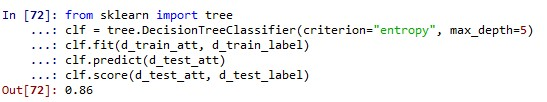
\includegraphics[scale=0.5]{figures/n3b.jpg}
		\caption{Lusia-Decission Tree Katty Perry}
		\label{contoh}
		\end{figure}
	\par Dalam gambar Decission Tree dijelaskan bahwa library tree dari sklearn. Dan mendifinisikan variable untuk memanggil Decission Tree Classifisier yang kemudian dilakukan fit atau pengujian. Lalu menggunakan prediksi dengan fungsi predict untuk memprediksi test. Yang terakhir memunculkan akurasi prediksi yaitu 0,86.
	\end{itemize}

\item Klasifikasikan dari data vektorisasi dengan klasifikasi SVM
	\par Berikut adalah klasifikasikan dari data vektorisasi dengan klasifikasi SVM
		\begin{figure}[ht]
		\centering
		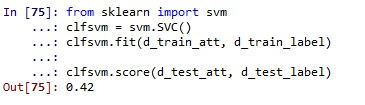
\includegraphics[scale=0.5]{figures/n4.jpg}
		\caption{Lusia-Hasil klasifikasi SVM}
		\label{contoh}
		\end{figure}
	\par Dalam gambar SVM dijelaskan bahwa mula-mula file svm diimpor dari sklearn, lalu melakukan fit dari d train att dan d train label atau disebut dengan pengujian. Selanjutnya variable didifinisikan variable untuk melakukan prediksi dataset dengan SVM. Dan yang terakhir muncul hasilnya yaitu 0,42.
	
\item Klasifikasikan dari data vektorisasi dengan klasifikasi Decission Tree
	\par Maksud dari gambar vektorisasi adalah hasil dari impor dataset
	\par Berikut adalah Decission Tree
		\begin{figure}[ht]
		\centering
		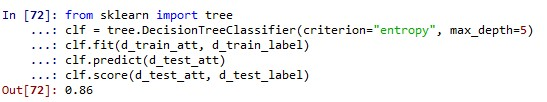
\includegraphics[scale=0.5]{figures/n3b.jpg}
		\caption{Lusia-Decission Tree}
		\label{contoh}
		\end{figure}
	\par Dalam gambar Decission Tree dijelaskan bahwa library tree dari sklearn. Dan mendifinisikan variable untuk memanggil Decission Tree Classifisier yang kemudian dilakukan fit atau pengujian. Lalu menggunakan prediksi dengan fungsi predict untuk memprediksi test. Yang terakhir memunculkan akurasi prediksi yaitu 0,86.

\item Plot confusion matrix
	\par Berikut adalah hasil dari ploting confusion matrix
		\begin{figure}[ht]
		\centering
		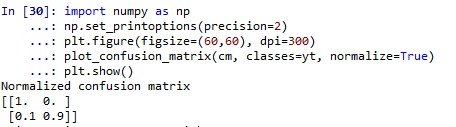
\includegraphics[scale=0.5]{figures/n6.jpg}
		\caption{Lusia-ploting confusion matrix}
		\label{contoh}
		\end{figure}
	\par Dari gambar dijelaskan bahwa library numpy di import sebagai np. Lalu 	Opsi set printoption untuk menentukan cara angka floating point, array dan objek NumPy lainnya ditampilkan. Selanjutnya matplotlib pyplot figure untuk membuat figur atau gambar baru. Selanjutnya confution matrix dinormalisasikan. Dan yang terakhir hasil ditampilkan.

\item Program cross validation
	\par Berikut adalah hasil dari program cross validation
		\begin{figure}[ht]
		\centering
		\includegraphics[scale=0.5]{figures/n7.jpg}
		\caption{Lusia-Program cross validation}
		\label{contoh}
		\end{figure}
		
	\par Maksud dari hasil gambar tersebut adalah untuk mendefinisikan dataset untuk 'menguji' model.
	
\item Program pengamatan komponen informasi
	\par Berikut adalah hasil dari program pengamatan komponen informasi
		\begin{figure}[ht]
		\centering
		\includegraphics[scale=0.5]{figures/n8.jpg}
		\caption{Lusia-Program pengamatan komponen informasi}
		\label{contoh}
		\end{figure}
		
	\par Maksud dari hasil gambar tersebut adalah diagram informasi dari dataset yang digunakan.

\end{enumerate}

\subsection{Penanganan Error}
\begin{enumerate}
	\item skrinsut error
		\begin{figure}[ht]
		\centering
		\includegraphics[scale=0.5]{figures/o1.jpg}
		\caption{Lusia-skrinsut error}
		\label{contoh}
		\end{figure}
	\item Tuliskan kode eror dan jenis errornya
		\begin{itemize}
		\item Kode error = KeyError: 'test preparation course'
		\item Jenis error = KeyError
		\end{itemize}
	\item Solusi pemecahan masalah error
		\par Solusinya adalah dengan memasukkan salah satu atribut dari dataset file csv yang digunakan.
\end{enumerate}





\par
\par

\section{Rahmi Roza-1164085}
\subsection{Teori}
Penjelasan Tugas Harian 7 ( No 1-6 )
\begin{enumerate}
\item Pengertian Klasifikasi Teks Dan Ilustrasi Gambar
\begin{itemize}
\item Pengertian Klasifikasi Teks
\par Klasifikasi teks adalah proses proses pengelompokkan bendaberdasarkan ciri-ciri persamaan dan perbedan dengan pemberian tag atau kategori ke teks sesuai dengan isinya. 
\par
\item Ilustrasi Gambar
\par Penjelasan : Berdasarkan pengertian diatas, ada beberapa contoh yang bisa diterapkan. Untuk salah satu contoh dari klasifikasi data sendiri dapat diliat pada gambar berikut \ref{ktRoza}.
\begin{figure}[!hbtp]
\centering
\includegraphics[scale=0.3]{figures/ktRoza.png}
\caption{Klasifikasi Teks Roza}
\label{text-fadila}
\end{figure}
\par
\end{itemize}
\par
\par
\item Mengapa Klasifikasi Bunga Tidak Bisa Menggunakan Machine Learning Dan Ilustrasi Gambar
\begin{itemize}
\item  Mengapa Klasifikasi Bunga Tidak Bisa Menggunakan Machine Learning
\par Penjelasan : Klasifikasi bunga tidak bisa digunakan pada machine learning karena terdapat masalah input yang sama dan output yang berbeda. Output atau error disebut noise.
\par
\item Ilustrasi Gambar
\par Penjelasan : Berdasarkan pengertian diatas, ada beberapa contoh yang bisa diterapkan. Untuk salah satu contoh dari klasifikasi bunga sendiri dapat diliat pada gambar berikut \ref{flowerRoza}.
\begin{figure}[!hbtp]
\centering
\includegraphics[scale=0.3]{figures/flowerRoza.jpg}
\caption{Klasifikasi Bunga Roza}
\label{text-fadila}
\end{figure}
\par
\end{itemize}
\par
\par
\item Teknik Pembelajaran Mesin Pada Teks Pada Kata-Kata Yang Digunakan Di Youtube Dan Ilustrasi Gambar
\begin{itemize}
\item  Teknik Pembelajaran Mesin Pada Teks Pada Kata-Kata Yang Digunakan Youtube
\par Penjelasan : Penggunaan Machine Learning pada Youtube yaitu contohnya pada saat kita melakukan searching vidio atau pun bahan lainnya di youtube maka yang akan ditampilkan adalah vidio dari keyword yang kita ketikkan di kotak pencarian. Dengan kata lain Youtube akan mempfilter vidio dengan keywoard yang telah digunakan. Dan pada saat kita menonton Youtube pada bagian sebelah kanan tampilan youtubr terdapat vidio yang berkaitan dengan keyworad yang kita cari tadi. Dimana disitulah Machine Learning pada Youtube menyimpan data.
\par
\item Ilustrasi Gambar
\par Penjelasan : Berdasarkan pengertian diatas, ada beberapa contoh yang bisa diterapkan. Untuk salah satu contoh dari Mesin Teks Youtube sendiri dapat diliat pada gambar berikut \ref{YoutubeRoza}.
\begin{figure}[!hbtp]
\centering
\includegraphics[scale=0.4]{figures/YoutubeRoza.png}
\caption{Youtube Roza}
\label{text-fadila}
\end{figure}
\par
\end{itemize}
\par
\par
\item Vektorisasi Data
\begin{itemize}
\item Maksud Dari Vektorisasi Data
\par Penjelasan : Pembagian dan pemecahan data, dan kemudian dilakukan perhitungan datanya. Vektorisasi juga dapat dimaksudkan dengan setiap data yang mungkin dipetakan ke integer tertentu. Yang mana data tersebut dalam bentuk data vektor diperoleh dalam bentuk koordinat titik yang menampilkan, menempatkan dan menyimpan data spasial dengan menggunakan titik, garis atau area (poligon). 
\par
\end{itemize}

\item Pengertian Bag Of Words Dan Ilustrasi Gambar
\begin{itemize}
\item  Pengertian Bag Of Words
\par Bag Of-Words adalah sebuah konsep yang diambil dari analisis teks yaitu mempresentasikan dokumen sebagai sebuah kantung informasi-infromasi penting tanpa mengurutkan setiap katanya.
\par
\item Ilustrasi Gambar
\par Penjelasan : Berdasarkan pengertian diatas, ada beberapa contoh yang bisa diterapkan. Untuk salah satu contoh dari Bag Of Words sendiri dapat diliat pada gambar berikut \ref{BagofwordsRoza.jpg}.
\begin{figure}[!hbtp]
\centering
\includegraphics[scale=0.2]{figures/BagofwordsRoza.jpg}
\caption{Bag of Words Roza}
\label{bag-fadila}
\end{figure}
\par
\end{itemize}
\par
\par

\item Pengertian TF-IDF Dan Ilustrasi Gambar
\begin{itemize}
\item  Pengertian TF-IDF
\par TF-IDF  (Term Frequency – Inverse Document Frequency) adalah  sebuah algoritma  adalah salah satu algoritma yang dapat digunakan untuk menganalisa hubungan antara sebuah frase/kalimat dengan sekumpulan dokumen. 
\par Inti utama dari algoritma ini adalah melakukan perhitungan nilai TF dan nilai IDF dari sebuah setiap kata kunci terhadap masing-masing dokumen. Nilai TF dihitung dengan rumus TF = jumlah frekuensi kata terpilih / jumlah kata dan nilai IDF dihitung dengan rumus IDF = log(jumlah dokumen / jumlah frekuensi kata terpilih). Selanjutnya adalah melakukan perkalian antara nilai TF dan IDF untuk mendapatkan jawaban akhir.
\item Ilustrasi Gambar
\par Penjelasan : Berdasarkan pengertian diatas, ada beberapa contoh yang bisa diterapkan. Untuk salah satu contoh dari TF-IDF sendiri dapat diliat pada gambar berikut \ref{TFIDFroza.jpeg}.
\begin{figure}[!hbtp]
\centering
\includegraphics[scale=0.2]{figures/TFIDFroza.jpeg}
\caption{TF-ID Rroza}
\label{tf-fadila}
\end{figure}
\par
\end{itemize}
\par
\par

\subsection{Praktek}
\begin{enumerate}
\item Membuat Aplikasi Sederhana menggunakan pandas, dan membuat data dummy sebnayak 500 baris dan melakukan data load ke data frame panda. Jelaskan arti perbaris!
\begin{figure}[!hbtp]
\centering
\includegraphics[scale=0.8]{figures/kodinganroza1.jpg}
\caption{Nomor 1 Roza}
\label{text-fadila}
\end{figure}
\begin{itemize}
\item Baris 1: Memanggil library pandas sebagai pd
\item Baris 2: Membaca dataset Balance Scale 
\item Baris 3:Mengambil data frame dari library pandas
\item Baris 4: Data Dummy digunakan untuk mengubah Categorical menjadi Integer
\item Baris 5: Menampilkan 5 data teratas
\par
\end{itemize}
\item GAMBAR HASIL No1:
\begin{figure}[!hbtp]
\centering
\includegraphics[scale=0.7]{figures/hasil1a.jpg}
\caption{Hasil 1 Roza}
\label{text-fadila}
\end{figure}
\begin{figure}[!hbtp]
\centering
\includegraphics[scale=0.9]{figures/hasil1b.jpg}
\caption{Hasil 1 Roza}
\label{text-fadila}
\end{figure}
\par

\item Membuat Aplikasi Sederhana menggunakan pandas, dan membuat data dummy sebnayak 500 baris dan melakukan data load ke data frame panda. Jelaskan arti perbaris.
\begin{itemize}
\begin{figure}[!hbtp]
\centering
\includegraphics[scale=0.7]{figures/kodinganroza2.jpg}
\caption{Nomor 2 Roza}
\label{text-fadila}
\end{figure}
\item Baris 1: Membagi data set balance scale dari 500 data menjadi data train menjadi 450 data.
\item Baris 2: Membagi data set balance scale dari sisa pembagian data train menjadi data test menjadi 50 data.
\par
\begin{figure}[!hbtp]
\centering
\includegraphics[scale=0.5]{figures/hasil2roza.jpg}
\caption{Hasil 2 Roza}
\label{text-fadila}
\end{figure}
\end{itemize}
\par

\item Vektorisasi dan Klasifikasi Data Dengan Decission Tree
\begin{itemize}
\begin{figure}[!hbtp]
\centering
\includegraphics[scale=0.7]{figures/kodinganroza3.jpg}
\caption{Nomor 3 Roza}
\label{text-fadila}
\end{figure}
\begin{figure}[!hbtp]
\centering
\includegraphics[scale=0.7]{figures/kodinganroza3_.jpg}
\caption{Hasil 3 Roza}
\label{text-fadila}
\end{figure}
\item Penjelasan:
\item Dalam in 11 impor tree dari sklearn. Dan mendefinisikan variabel clf untuk memanggil Decission Tree Classifier dan melakukan fit atau pengujian.
\item Dalam in 12 menggunakan prediksi untk clf dengan function predict untuk memprediksi test. Dan hasilnya muncul dalam bentuk array.
\item clf score memunculkan akurasi prediksi yang dilakukan terhadap clf
\end{itemize}
\par

\item Klasifikasi SVM
\begin{itemize}
\begin{figure}[!hbtp]
\centering
\includegraphics[scale=0.7]{figures/kodinganroza4.jpg}
\caption{Nomor 4 Roza}
\label{text-fadila}
\end{figure}
\item Import SVM dari  sklearn
\item Melakukan fit dari d train att dan d train label atau disebut denga pengujian
\item Mendefinisikan variabel df untuk melakukan prediksi dataset Youtube LMFAO dengan SVM. Dan akan muncul hasil prediksinya 
\end{itemize}
\par

\item Klasifikasi Decision Tree
\begin{itemize}
\begin{figure}[!hbtp]
\centering
\includegraphics[scale=0.9]{figures/kodinganroza5.jpg}
\caption{Nomor 5 Roza}
\label{text-fadila}
\end{figure}
\item Penjelasan:
\item Dalam in 17 impor tree dari sklearn. Dan mendefinisikan variabel clf untuk memanggil Decission Tree Classifier dan melakukan fit atau pengujian.
\item menggunakan prediksi untk clf dengan function predict untuk memprediksi test. Dan hasilnya muncul dalam bentuk array.
\item clf score memunculkan akurasi prediksi yang dilakukan terhadap clf
\end{itemize}
\par

\item Matplotlib
\begin{itemize}
\begin{figure}[!hbtp]
\centering
\includegraphics[scale=0.5]{figures/kodinganroza6.jpg}
\caption{Nomor 6 Roza}
\label{text-fadila}
\end{figure}
\item Penjelasan:
\par Fungsi ini mencetak dan memplot Confussion Matrix. Normalisasi dapat diterapkan dengan mengatur `normalize = True`. Ada Confussion Matrik menggunakan normalisasi dan ada confussion matrik tidak menggunakan normalisasi.
\end{itemize}
\par

\item Menjelaskan Program Cross Validation
\begin{itemize}
\begin{figure}[!hbtp]
\centering
\includegraphics[scale=0.5]{figures/kodinganroza7.jpg}
\caption{Nomor 7 Roza}
\label{text-fadila}
\end{figure}
\item Penjelasan: Variabel score akan melakukan cross validation pada variabel clf, d train att, dan train label. Variabel skorrata2 akan menghitung nilai rata-rata dari  variabel scores tadi menggunakan function mean. Dan scoresd menghitung standar deviasi dari data yang diberikan.
\par
\item GAMBAR HASIL No7:
\begin{figure}[!hbtp]
\centering
\includegraphics[scale=0.5]{figures/hasilno7.jpg}
\caption{Hasil 7 Roza}
\label{text-fadila}
\end{figure}
\begin{figure}[!hbtp]
\centering
\includegraphics[scale=0.5]{figures/hasilno7b.jpg}
\caption{Hasil 7 Roza}
\label{text-fadila}
\end{figure}
\end{itemize}
\par

\item Program Pengamatan Komponen
\begin{itemize}
\begin{figure}[!hbtp]
\centering
\includegraphics[scale=0.5]{figures/kodingan8.jpg}
\caption{Nomor 8 Roza}
\label{text-fadila}
\end{figure}
\begin{figure}[!hbtp]
\centering
\includegraphics[scale=0.5]{figures/kodinganroza8.jpg}
\caption{Nomor 8 Roza}
\label{text-fadila}
\end{figure}
\item Penjelasan: Pada gambar pertama merupakan kodingan untuk mencetak data dari maxfeatures, num estimators dan accuracy. Sedangkan pada gambar yang kedua itu merupakan gambarnya. Atau hasil gambarnya.
\par 
\end{itemize}
\par

\subsection{Penanganan Error}
\begin{enumerate}
\item Skrinsut Error
\begin{figure}[ht]
\centering
\includegraphics[scale=0.5]{figures/erorque.jpg}
\caption{ Error Roza}
\label{6}
\end{figure}
\item Kode Error dan Jenis Errornya
\par Kode Error: "FileNotFoundError" dan "File b 'balancee.csv' does not exist". 
\par Jenis Error: Import Dataset
\item Penanganan
\par Import ulang dataset dan sesuaikan dengan letak dataset pada file explorer.

\end{enumerate}
\end{enumerate}

\end{enumerate}





\par
\par
\section{Fadila-1164072}
\subsection{Teori}
Penjelasan Tugas Harian 7 ( No 1-6 )
\begin{enumerate}
\item Pengertian Klasifikasi Teks Dan Ilustrasi Gambar
\begin{itemize}
\item Pengertian Klasifikasi Teks
\par Klasifikasi teks adalah proses pemberian tag atau kategori ke teks sesuai dengan isinya. Teks dapat menjadi sumber informasi yang sangat kaya, tetapi mengekstraksi wawasan darinya bisa sulit dan memakan waktu karena sifatnya yang tidak terstruktur.
\par
\item Ilustrasi Gambar
\par Penjelasan : Berdasarkan pengertian diatas, ada beberapa contoh yang bisa diterapkan. Untuk salah satu contoh dari klasifikasi data sendiri dapat diliat pada gambar berikut \ref{text-fadila}.
\begin{figure}[!hbtp]
\centering
\includegraphics[scale=0.3]{figures/text-fadila.jpg}
\caption{text-fadila}
\label{text-fadila}
\end{figure}
\par
\end{itemize}
\par
\par
\item Mengapa Klasifikasi Bunga Tidak Bisa Menggunakan Machine Learning Dan Ilustrasi Gambar
\begin{itemize}
\item  Mengapa Klasifikasi Bunga Tidak Bisa Menggunakan Machine Learning
\par Penjelasan : Untuk klasifikasi bunga tidak dapat menggunakan machine learning dikarenakan memiliki masalah input yang sama namun keluarannya (output) yang berbeda, biasanya output atau error ini disebut dengan istilah 'noise'. Noise sendiri merupakan output yang disimpan / ditangkap maupun direkam bukan seperti seharusnya ( keluaran yang diiginkan ). 
\par Apabila diberikan contoh, maka contohnya yaitu kita berasumsi secara implisit bahwa klarifikasi bunga yang kita lakukan sudah tepat dan kita melakukannya seperti seorang ahli tanaman. Namun pada hasilnya masih saja terjadi kesalahan. Selain itu, selalu ada peluang untuk memperkenalkan kesalahan saat merekam ataupun menyimpan data, maka harus dilakukan penelitian yang lebih rinci sehingga tidak menimbulkan 'noise' itu sendiri.
\par
\item Ilustrasi Gambar
\par Penjelasan : Berdasarkan pengertian diatas, ada beberapa contoh yang bisa diterapkan. Untuk salah satu contoh dari klasifikasi bunga sendiri dapat diliat pada gambar berikut \ref{bunga-fadila}.
\begin{figure}[!hbtp]
\centering
\includegraphics[scale=0.3]{figures/bunga-fadila.jpg}
\caption{bunga-fadila}
\label{bunga-fadila}
\end{figure}
\par
\end{itemize}
\par
\par
\item Teknik Pembelajaran Mesin Pada Teks Pada Kata-Kata Yang Digunakan Di Youtube Dan Ilustrasi Gambar
\begin{itemize}
\item  Teknik Pembelajaran Mesin Pada Teks Pada Kata-Kata Yang Digunakan Youtube
\par Penjelasan : Kita ambil sebuah kasus yang semua orang telah ketahui dan juga pahami. Kasus tersebut yaitu perekomendasian video dari pencarian menggunakan "text / kata" di  Youtube. Pada saat menggunakan Youtube terdapat Machine Learning yang bekerja dan memproses perintah ataupun aktivitas tersebut, dimana akan memfilter secara otomatis video yang disesuaikan dengan "keyword" yang kita masukkan sehingga memberikan keluaran video dengan keyword yang benar. 
\par Adapula fitur yang di dapatkan ketika sedang menonton Youtube. Tampilan sebelah kanan terdapat pilihan 'Next' atapun 'Suggestion' yang menam-pilkan beberapa video serupa sesuai dengan yang dicari atau sedang ditonton. Ketika mengklik salah satu video dari baris tersebut, maka Youtube akan mengingat dan menggunakan kata yang tertera sebagai referensi kembali sehingga akan memberikan kemudahan pada pencarian yang lainnya, Dan disitulah mesin belajar sendiri dan menyimpan data secara berkala sehingga berkembang. 
\par
\item Ilustrasi Gambar
\par Penjelasan : Berdasarkan pengertian diatas, ada beberapa contoh yang bisa diterapkan. Untuk salah satu contoh dari Mesin Teks Youtube sendiri dapat diliat pada gambar berikut \ref{youtube-fadila}.
\begin{figure}[!hbtp]
\centering
\includegraphics[scale=0.25]{figures/youtube-fadila.jpg}
\caption{youtube-fadila}
\label{youtube-fadila}
\end{figure}
\par
\end{itemize}
\par
\par
\item Vektorisasi Data
\begin{itemize}
\item Maksud Dari Vektorisasi Data
\par Penjelasan : Pembagian dan pemecahan data, kemudian dilakukan perhitungan. Vektorisasi juga dapat dimaksudkan dengan setiap data yang mungkin dipetakan ke integer tertentu. jika kita memiliki array yang cukup besar maka setiap kata / data cocok dengan slot unik dalam array (nilai pada indeks adalah nomor satu kali kata itu muncul).
\par Array angka floating point ( Mewakili data ) :
\begin{itemize}
\item teks
\item audio
\item gambar
\end{itemize}
\par Contoh : -[1.0, 0.0, 1.0, 0.5]
\par
\end{itemize}
\par
\par
\item Pengertian Bag Of Words Dan Ilustrasi Gambar
\begin{itemize}
\item  Pengertian Bag Of Words
\par bag-of-words adalah representasi penyederhanaan yang digunakan dalam pemrosesan bahasa alami dan pengambilan informasi. Model bag-of-words sederhana untuk dipahami dan diterapkan dan telah melihat kesuksesan besar dalam masalah seperti pemodelan bahasa dan klasifikasi dokumen ( penyelesaian dll ).
\par
\par
\item Ilustrasi Gambar
\par Penjelasan : Berdasarkan pengertian diatas, ada beberapa contoh yang bisa diterapkan. Untuk salah satu contoh dari Bag Of Words sendiri dapat diliat pada gambar berikut \ref{bag-fadila}.
\begin{figure}[!hbtp]
\centering
\includegraphics[scale=0.3]{figures/bag-fadila.jpg}
\caption{bag-fadila}
\label{bag-fadila}
\end{figure}
\par
\end{itemize}
\par
\par
\item Pengertian TF-IDF Dan Ilustrasi Gambar
\begin{itemize}
\item  Pengertian TF-IDF
\par TF-IDF atau TFIDF, adalah kependekan dari istilah frekuensi dokumen terbalik, dimana merupakan statistik numerik yang dimaksudkan untuk mencerminkan betapa pentingnya sebuah kata untuk sebuah dokumen dalam kumpulan atau kumpulan.
\par Nilai tf-idf meningkat secara proporsional dengan berapa kali sebuah kata muncul dalam dokumen dan diimbangi dengan jumlah dokumen dalam korpus yang mengandung kata, yang membantu menyesuaikan fakta bahwa beberapa kata muncul lebih sering secara umum
\item Ilustrasi Gambar
\par Penjelasan : Berdasarkan pengertian diatas, ada beberapa contoh yang bisa diterapkan. Untuk salah satu contoh dari TF-IDF sendiri dapat diliat pada gambar-gambar berikut \ref{tf2-fadila}.
\begin{figure}[!hbtp]
\centering
\includegraphics[scale=0.4]{figures/tf2-fadila.jpg}
\caption{tf2-fadila}
\label{tf2-fadila}
\end{figure}
\par
\par
\end{itemize}
\par
\par

\end{enumerate}


\par
\par
\subsection{Praktek Fadila}
Pengerjaanya Tugas Harian 8 ( No 1-8 )
\begin{enumerate}
\item Pembuatan Aplikasi Pandas Sederhana Dengan Menggunakan Dataset berisi 500 baris data.
\begin{itemize}
\item Penjelasan Code Pandas Sederhana
\begin{lstlisting}
import pandas as pd
fadila_car = pd.read_csv('1.csv', sep=';')
len(fadila_car)

fadila = pd.DataFrame(fadila_car, columns = ['buying', 'maint', 'doors', 'persons', 'lug-boot', 'safety', 'class'])

dummy = pd.get_dummies (fadila['class'])
dummy.head()
\end{lstlisting}
\begin{enumerate}
\item Baris 1 : Mengimport Library Pandas sebagai pd
\item Baris 2 : Membuat variabel fadila\_car dimana membaca dataset berupa format csv "1.csv" dengan separator.
\item Baris 3 : Menampilkan hasil dari variabel fadila\_car ( berupa jumlah/angka karena len )
\item Baris 4 : Membuat variabel fadila dimana mengambil/ memanggil DataFrame dari library pd ( pandas ) dengan parameter variabel.
\item Baris 5 : Mendefinisikan variabel dummy dimana memanggil get\_dummies dari pd dengan parameter variabel fadila dan column class
\item Baris 6 : Menampilkan 5 data teratas pada kolom class dari variabel fadila
\end{enumerate}
\item Hasil Dari Aplikasi Sederhana Code Pandas
\par Penjelasan : Hasilnya dapat diliat pada gambar berikut \ref{1-fadila}, \ref{lanjutan1-fadila}, \ref{lanjutan1-1-fadila} dan \ref{lanjutan1-2-fadila}.
\begin{figure}[!hbtp]
\centering
\includegraphics[scale=0.3]{figures/1-fadila.jpg}
\caption{1-fadila}
\label{1-fadila}
\end{figure}
\par
\par
\begin{figure}[!hbtp]
\centering
\includegraphics[scale=0.3]{figures/lanjutan1-fadila.jpg}
\caption{lanjutan1-fadila}
\label{lanjutan1-fadila}
\end{figure}
\par
\par
\begin{figure}[!hbtp]
\centering
\includegraphics[scale=0.3]{figures/lanjutan1-1-fadila.jpg}
\caption{lanjutan1-1-fadila}
\label{lanjutan1-1-fadila}
\end{figure}
\par
\par
\begin{figure}[!hbtp]
\centering
\includegraphics[scale=0.2]{figures/lanjutan1-2-fadila.jpg}
\caption{lanjutan1-2-fadila}
\label{lanjutan1-2-fadila}
\end{figure}
\end{itemize}
\par
\par
\item Pemecahan dataframe menjadi dua dataframe yaitu 450 row pertama dan 50 data sisa.
\begin{itemize}
\item Dataframe 1 : 450 row data pertama
\item Dataframe 2 : 50 row data sisanya.
\item Codingan Dan Penjelasannya :
\begin{lstlisting}
fadila_car_train = fadila_car[:450]
fadila_car_test = fadila_car[451:]
\end{lstlisting}
\begin{enumerate}
\item Baris 1 : Membuat variabel fadila\_car\_train dari variabel fadila\_car dengan 450 data awal untuk dijadikan data training
\item Baris 2 : Membuat variabel fadila\_car\_test dari variabel fadila\_car dengan 50 data sisanya untuk data testing ( dimulai dari data ke 451 sampai akhir data )
\end{enumerate}
\item Hasil Dari Pemecahan Dataframe
\par Penjelasan : Hasilnya dapat diliat pada gambar berikut \ref{2-fadila} dan \ref{lanjutan2-fadila}.
\begin{figure}[!hbtp]
\centering
\includegraphics[scale=0.3]{figures/2-fadila.jpg}
\caption{2-fadila}
\label{2-fadila}
\end{figure}
\par
\par
\begin{figure}[!hbtp]
\centering
\includegraphics[scale=0.3]{figures/lanjutan2-fadila.jpg}
\caption{lanjutan2-fadila}
\label{lanjutan2-fadila}
\end{figure}
\par 
\par 
\end{itemize}
\par
\par
\item Vektorisasi Klasifikasi Data NPM mod 4 ( Katy Perry) Dengan Decision Tree
\par
\begin{lstlisting}
from sklearn import tree
clf = tree.DecisionTreeClassifier(criterion="entropy", max_depth=5)
clf = clf.fit(d_train_att, d_train_label)
\end{lstlisting}
\par Penjelasan : Sesuai Hasil.
\begin{enumerate}
\item Dalam [ in 21 ] merupakan hasil dari impor tree dari sklearn. Dan mendefinisikan variabel clf untuk memanggil Decission Tree Classifier dan melakukan fit atau pengujian.
\item Dalam [ in 22 ] menjelaskan bahwa digunakan prediksi untk clf dengan function predict untuk memprediksi test. Dan hasilnya muncul dalam bentuk array.
\item Kemudian Dalam [ in 23 ] clf score memunculkan akurasi prediksi yang dilakukan terhadap clf
\end{enumerate}
\par
\begin{itemize}
\item Hasil Program Menggunakan Decision Tree
\par Hasilnya dapat diliat pada gambar berikut \ref{3-fadila}.
\begin{figure}[!hbtp]
\centering
\includegraphics[scale=0.3]{figures/3-fadila.jpg}
\caption{3-fadila}
\label{3-fadila}
\end{figure}
\par
\par
\par
\end{itemize}
\par
\par
\item Vektorisasi Dengan Klasifikasi SVM
\par
\begin{lstlisting}
from sklearn import svm
clfsvm = svm.SVC()
clfsvm.fit(d_train_att, d_train_label)

clfsvm.score(d_test_att, d_test_label)
\end{lstlisting}
\par Penjelasan :
\begin{enumerate}
\item Dilakukan pengimportan module SVM dari sklearn
\item Selanjutnya melakukan fit dari d train att dan d train label atau disebut denga pengujian
\item Mendefinisikan variabel df untuk melakukan prediksi dataset Youtube Katy Perry dengan SVM. Dan akan muncul hasil prediksinya seperti pada contoh gambarnya
\end{enumerate}
\par
\begin{itemize}
\item Hasil Klasifikasi SVM
\par Hasilnya dapat diliat pada gambar berikut \ref{4-fadila}.
\begin{figure}[!hbtp]
\centering
\includegraphics[scale=0.3]{figures/4-fadila.jpg}
\caption{4-fadila}
\label{4-fadila}
\end{figure}
\par
\par
\par
\end{itemize}
\par
\par
\par
\item Vektorisasi Menggunakan Klasifikasi Decision Tree
\par
\begin{lstlisting}
from sklearn import tree
clf = tree.DecisionTreeClassifier()
clf = clf.fit(d_train_att, d_train_label)
clf.predict(d_test_att)
clf.score(d_test_att,d_test_label)
\end{lstlisting}
\par Penjelasan :
\begin{enumerate}
\item Dalam [ in 31 ] merupakan hasil dari impor tree dari sklearn. Dan mendefinisikan variabel clf untuk memanggil Decission Tree Classifier dan melakukan fit atau pengujian.
\item Di dalamnya juga menjelaskan bahwa digunakan prediksi untk clf dengan function predict untuk memprediksi test. Dan hasilnya muncul dalam bentuk array.
\item clf score memunculkan akurasi prediksi yang dilakukan terhadap clf
\item Lalu muncul lah hasilnya pada [ out 31 ] seperti pada gambar
\end{enumerate}
\begin{itemize}
\item Hasil Program Cross Validation
\par  Hasilnya dapat diliat pada gambar berikut \ref{5-fadila}.
\begin{figure}[!hbtp]
\centering
\includegraphics[scale=0.3]{figures/5-fadila.jpg}
\caption{5-fadila}
\label{5-fadila}
\end{figure}
\par
\par
\par
\end{itemize}
\par
\par
\item Plot Confusion Matrix
\begin{itemize}
\item Code Plot Confusion Matrix
\begin{figure}[!hbtp]
\centering
\includegraphics[scale=0.2]{figures/cod6-fadila.jpg}
\caption{cod6-fadila}
\label{cod6-fadila}
\end{figure}
\par Penjelasan : Untuk gambar \ref{cod6-fadila} yang ditampilkan / diperlihatkan telah dieksekusi dimana fungsi code tersebut yaitu untuk mencetak dan memplot Confussion Matrix. Normalisasi dapat diterapkan dengan mengatur `normalize = True`. Ada Confussion Matrik menggunakan normalisasi dan ada confussion matrik tidak menggunakan normalisasi.
\item Hasil Plot Confusion Matrix
\par Hasilnya dapat diliat pada gambar berikut \ref{6-fadila} dan \ref{lanjutan6-fadila} .
\begin{figure}[!hbtp]
\centering
\includegraphics[scale=0.2]{figures/6-fadila.jpg}
\caption{6-fadila}
\label{6-fadila}
\end{figure}
\par
\par
\begin{figure}[!hbtp]
\centering
\includegraphics[scale=0.25]{figures/lanjutan6-fadila.jpg}
\caption{lanjutan6-fadila}
\label{lanjutan6-fadila}
\end{figure}
\par
\end{itemize}
\par
\par
\item Program Cross Validation
\begin{lstlisting}
from sklearn.model_selection import cross_val_score
scores = cross_val_score(clf,d_train_att,d_train_label,cv=5)

skorrata2=scores.mean()
skoresd=scores.std()
\end{lstlisting}
\par Penjelasan :  Pada codingan maupun hasil dari cross validation berikut, menjelaskan dimana variabel score akan melakukan cross validation pada variabel clf, d train att, dan train label. Variabel skorrata2 akan menghitung nilai rata-rata dari variabel scores tadi menggunakan function mean. Dan scoresd menghitung standar deviasi dari data yang diberikan.
\begin{itemize}
\item Hasil Program Cross Validation
\par Hasilnya dapat diliat pada gambar berikut \ref{7-fadila} dan \ref{lanjutan7-fadila} .
\begin{figure}[!hbtp]
\centering
\includegraphics[scale=0.3]{figures/7-fadila.jpg}
\caption{7-fadila}
\label{7-fadila}
\end{figure}
\par
\begin{figure}[!hbtp]
\centering
\includegraphics[scale=0.3]{figures/lanjutan7-fadila.jpg}
\caption{lanjutan7-fadila}
\label{lanjutan7-fadila}
\end{figure}
\par
\end{itemize}
\par
\par
\par
\item Program Pengamatan Komponen Informasi
\begin{itemize}
\item Hasil Dan Code Pengamatan Komponen Informasi :
\par Hasilnya dapat diliat pada gambar berikut \ref{8-fadila} dan \ref{lanjutan8-fadila}.
\begin{figure}[!hbtp]
\centering
\includegraphics[scale=0.3]{figures/8-fadila.jpg}
\caption{8-fadila}
\label{8-fadila}
\end{figure}
\par
\par
\begin{figure}[!hbtp]
\centering
\includegraphics[scale=0.3]{figures/lanjutan8-fadila.jpg}
\caption{lanjutan8-fadila}
\label{lanjutan8-fadila}
\end{figure}
\par
\end{itemize}
\par Penjelasan :
\begin{enumerate}
\item Max featuresnya dari range 1 sampai 10
\item Untuk n estimators dengan range 2 sampai 40
\item Kemudian pada variabel rf params berisikan function np empty dimana akan membuat array baru berisikan tipe yang didefinisikan dengan random value
\item Mendefinisikan nilai i dimulai dari angka 0 dimana max features dan n estimators menggunakan klasifikasi randomforestclassifier menggunakan data prediksi.
\item Mendefinisikan rfparams untuk max features , n estimators, nilai rata dan std
\item Hasil (komponen informasi) juga ditampilkan dalam bentuk/module/ matplotlib
\item Secara keseluruhan untuk variabel x, y dan z dilakukan penyettingan dengan parameternya masing-masing
\item Label pun di definisikan untuk setiap variabelnya
\item Dan hasil keseluruhan akan nampak seperti pada gambar yang mengambarkan komponen informasi secara lengkap
\end{enumerate}
\par
\par
\par
\end{enumerate}


\par
\par
\par
\subsection{Penanganan Error Fadila}
Menangani dan Mengatasi Error Pada Praktek
\begin{enumerate}
\item Error 1 :
\begin{itemize} 
\item Code Yang Error :
\begin{lstlisting}
import pandas as pd
d = pd.read_csv("dataset/Youtube02-KatyPerry.csv")
\end{lstlisting}
\item Peringatan Error :
\begin{lstlisting}
FileNotFoundError: File b'dataset/Youtube02-KatyPerry.csv' does not exist
\end{lstlisting}
\item Gambar Error 1 : ( Lebih jelas )
\begin{figure}[!hbtp]
\centering
\includegraphics[scale=0.3]{figures/e1-fadila.jpg}
\caption{error1-fadila}
\label{error1-fadila}
\end{figure}
\begin{itemize}
\item Cara Penanganan :
\begin{enumerate}
\item Pada Codingan yang dieksekusi sebenarnya untuk membaca dataset dari Youtube02-KatyPerry.csv
\item Namun, terdapat error dan hal tersebut disebabkan karena file codingan yang dieksekusi tidak berada pada folder yang sama dengan dataset Katy Perry.
\item Silahkan tuliskan codingan berikut untuk mengganti codingan yang bermasalah
\begin{lstlisting}
import pandas as pd
d = pd.read_csv("Youtube02-KatyPerry.csv")
\end{lstlisting}
\item Dengan menganti codingan tersebut, maka tidak akan terjadi error lagi.
\par
\par
\end{enumerate}
\end{itemize}
\end{itemize}
\end{enumerate}


\subsection{Praktek}
\chapter{Conclusion}
brief of conclusion

\section{Conclusion of Problems}
Tell about solving the problem

\section{Conclusion of Method}
Tell about solving using method

\section{Conclusion of Experiment}
Tell about solving in the experiment

\section{Conclusion of Result}
tell about result for purpose of this research.



\section{Rahmi Roza-1164085}
\subsection{Praktek}
Praktek Tugas Harian 
\begin{enumerate}

\item Mengapa Kata-Kata Harus di Vektorisasi
\par Kata harus di vektorisasi dikarenakan mesin hanya mampu membaca data dalam bentuk angka. Oleh karena itu diperlukan vektorisasi kata agar mesin mampu membaca data yang telah di vektorisasi. 
\par
\begin{itemize}
\item Gambar :
\par Penjelasan : Berdasarkan pengertian diatas, ada beberapa contoh yang bisa diterapkan. Untuk salah satu contoh dari klasifikasi data sendiri dapat diliat pada gambar berikut \ref{vekktorisasikataroza}.
\begin{figure}[!hbtp]
\centering
\includegraphics[scale=0.6]{figures/vekktorisasikataroza.jpg}
\caption{Vektorisasi Kata Roza}
\label{text-fadila}
\end{figure}
\end{itemize}

\item Mengapa Dimensi Dari Vektor Dataset Google Bisa Sampai 300
\par Masing-masing nilai dalam vektor 300 dimensi yang terkait dalam sebua kata "dioptimalkan" dalam  beberapa hal untuk menangkap aspek yang  berbeda dari makna dan penggunaan kata itu.Dengan kata lain masing-masing dari 300 nilai sesuai dengan beberapa fitur abstrak kata. Menghapus kombinasi nilai-nilai ini secara acak akan menghasilkan vektor yang mungkin kurang informasi penting tentang kata tersebut dan mungkin tidak lagi berfungsi sebagai representasi yang baik dari kata itu. Atau singkat cerita mungkin ada lebih dari 3 miliar kata-kata dan kalimat atau data yang tidak mungkin disimpan dalam 1 diemensi vektor makan disimpan menjadi 300 dimensi vektor untuk mengurangi kegagalan memori.
\par
\begin{itemize}
\item Gambar :
\par Penjelasan : Berdasarkan pengertian diatas, ada beberapa contoh yang bisa diterapkan. Untuk salah satu contoh dari klasifikasi data sendiri dapat diliat pada gambar berikut \ref{googleroza}.
\begin{figure}[!hbtp]
\centering
\includegraphics[scale=0.4]{figures/googleroza.png}
\caption{Vektorisasi Kata Roza}
\label{text-fadila}
\end{figure}
\end{itemize}

\item Konsep Vektorisasi Kata 
\par Konsep vektorisasi data merupakan kata-kata yang di inputkan pada mesin learning. Dan outputan nya berupa kara-kata atau keyword dari pencarian yang tekah di lakukan sebelumnya. Contoh nya pada saat kita melakukan pencarian di channel youtube kita. Maka akan muncul hasil dari pencarian dari kata-kata yang telah kita cari.
\par
\begin{itemize}
\item Gambar :
\par Penjelasan : Berdasarkan pengertian diatas, ada beberapa contoh yang bisa diterapkan. Untuk salah satu contoh dari klasifikasi data sendiri dapat diliat pada gambar berikut \ref{vekktorisasikataroza}.
\begin{figure}[!hbtp]
\centering
\includegraphics[scale=0.5]{figures/vekktorisasikataroza.jpg}
\caption{Vektorisasi Kata Roza}
\label{text-fadila}
\end{figure}
\end{itemize}

\item Konsep Vektorisasi Dokumen 
\par Konsep vektorisasi dokumen yaitu mesin akan membaca terlebih dahulu semua kalimat yang ada di dalam dokumen da nanti kalimat yang ada di dalam dikumen tersebut akan di oecah menjadi kata-kata.
\par
\begin{itemize}
\item Gambar :
\par Penjelasan : Berdasarkan pengertian diatas, ada beberapa contoh yang bisa diterapkan. Untuk salah satu contoh dari klasifikasi data sendiri dapat diliat pada gambar berikut \ref{vektorisasidokroza}.
\begin{figure}[!hbtp]
\centering
\includegraphics[scale=0.7]{figures/vektorisasidokroza.png}
\caption{Vektorisasi Dokumen Roza}
\label{text-fadila}
\end{figure}
\end{itemize}

\item Mean dan Standar Deviasi
\par Mean adalah teknik penjelasan kelompok yang didasarkan atas nilai rata-rata dari kelompok tersebut. Rata-Rata (mean) ini didapat dengan menjumlahkan data seluruh individu dalam kelompok itu, kemudian dibagi dengan jumlah individu yang ada pada kelompok tersebut. Standar deviasi adalah nilai statistik yang digunakan untuk menentukan bagaimana sebaran data dalam sampel, dan seberapa dekat titik data individu ke mean – atau rata-rata – nilai sampel.Sebuah standar deviasi dari kumpulan data sama dengan nol menunjukkan bahwa semua nilai-nilai dalam himpunan tersebut adalah sama. Sebuah nilai deviasi yang lebih besar akan memberikan makna bahwa titik data individu jauh dari nilai rata-rata.
\par
\begin{itemize}
\item Gambar :
\par Penjelasan : Berdasarkan pengertian diatas, ada beberapa contoh yang bisa diterapkan. Untuk salah satu contoh dari klasifikasi data sendiri dapat diliat pada gambar berikut \ref{meanroza}.
\begin{figure}[!hbtp]
\centering
\includegraphics[scale=0.5]{figures/meanroza.png}
\caption{Mean Roza}
\label{text-fadila}
\end{figure}
\begin{figure}[!hbtp]
\centering
\includegraphics[scale=0.7]{figures/standarroza.png}
\caption{Standar Deviasi Roza}
\label{text-fadila}
\end{figure}
\par
\end{itemize}

\item Skip Gram
\par Skip-Gram mencoba memprediksi vektor kata-kata yang ada di konteks diberikan vektor kata tertentu. Skip-gram membuat sepasang kata target dan konteks sebagai sebuah instance sehingga skip-gram cenderung lebih baik ketika ukuran corpus sangat besar.
\par
\begin{itemize}
\item Gambar :
\par Penjelasan : Berdasarkan pengertian diatas, ada beberapa contoh yang bisa diterapkan. Untuk salah satu contoh dari klasifikasi data sendiri dapat diliat pada gambar berikut \ref{skipgramroza}.
\begin{figure}[!hbtp]
\centering
\includegraphics[scale=0.5]{figures/skipgramroza.png}
\caption{Skip-Gram Roza}
\label{text-fadila}
\end{figure}
\end{itemize}
\end{enumerate}

\begin{itemize}
\item Plagiarisme Roza
\begin{figure}[!hbtp]
\centering
\includegraphics[scale=0.5]{figures/plagiarismeroza.jpg}
\caption{Plagiarisme Roza}
\label{text-fadila}
\end{figure}
\end{itemize}


\chapter{MFCC dan Neutral Network}
Untuk pratikum saat ini menggunakan buku Python Artificial Intelligence Projects for Beginners. Dengan praktek menggunakan python 3 dan editor spyder dan library python keras dan librosa.

\section{Rahmi Roza-1164085}
\subsection{Teori}
\begin{enumerate}
\item Kenapa File Suara Harus Dilakukan MFCC
\begin{itemize}
\item Penjelasan: Agar bisa mengubah suara menjadi vektor. Sehingga data suara bisa diolah menjadi outputan. Jadi semua parameter inputan baik itu suara, dokumen harus dipersiapkan datanya terlebih dahulu, kalau untuk dokumen untuk teks menggunakan word2vec, sedangkan untuk suara menggunakan MFCC (Mel Frequency Cepstral Coeficients) 
\par 
\par
\item Ilustrasi Gambar
\begin{figure}[!hbtp]
\centering
\includegraphics[scale=0.7]{figures/mfccroza.jpg}
\caption{MFCC Roza}
\label{text-fadila}
\end{figure}
\par
\end{itemize}
\par
\par

\item Konsep Dasar Neural Network
\begin{itemize}
\item  Penjelasan:
\par Neural Network merupakan kategori ilmu Soft Computing. Neural Network sebenarnya mengadopsi dari kemampuan otak manusia yang mampu memberikan stimulasi/rangsangan, melakukan proses, dan memberikan output. Output diperoleh dari variasi stimulasi dan proses yang terjadi di dalam otak manusia. Kemampuan manusia dalam memproses informasi merupakan hasil kompleksitas proses di dalam otak. Misalnya, yang terjadi pada anak-anak, mereka mampu belajar untuk melakukan pengenalan meskipun mereka tidak mengetahui algoritma apa yang digunakan.
\par
\item Ilustrasi Gambar
\begin{figure}[!hbtp]
\centering
\includegraphics[scale=0.3]{figures/neuralroza.jpg}
\caption{Konsep Dasar Neural Network Roza}
\label{text-fadila}
\end{figure}
\par
\end{itemize}
\par
\par

\item Konsep Pembobotan Dalam Neural Network
\begin{itemize}
\item Penjelasan:
\par Cara kerja Neural Network dapat dianalogikan sebagaimana halnya manusia belajar dengan mengunakan contoh atau yang disebut sebagai supervised learning. Sebuah Neural Network dikonfigurasi untuk aplikasi tertentu, seperti pengenalan pola atau klasifikasi data, dan kemudian disempurnakan melalui proses pembelajaran. Proses belajar yang terjadi dalam sistem biologis melibatkan penyesuaian koneksi sinaptik yang ada antara neuron, dalam halnya pada Neural Network penyesuaian koneksi sinaptik antar neuron dilakukan dengan menyesuaikan nilai bobot yang ada pada tiap konektivitas baik dari input, neuron maupun output.
\par
\item Ilustrasi Gambar
\begin{figure}[!hbtp]
\centering
\includegraphics[scale=0.5]{figures/pemboobotanroza.jpg}
\caption{Konsep Pembobotan Roza}
\label{text-fadila}
\end{figure}
\par
\end{itemize}
\par
\par

\item Konsep Fungsi Aktivasi Dalam Neural Network
\begin{itemize}
\item Penjelasan:
\par Setiap neuron mempunyai tingkat aktivasi yang merupakan fungsi dari input yang masuk padanya. Aktivasi yang dikirim suatu neuron ke neuron lain berupa sinyal dan hanya dapat mengirim sekali dalam satu waktu, meskipun sinyal tersebut disebarkan pada beberapa neuron yang lain.
\par
\item Ilustrasi Gambar
\begin{figure}[!hbtp]
\centering
\includegraphics[scale=0.7]{figures/aktivasiroza.jpg}
\caption{Konsep Aktivasi Roza}
\label{text-fadila}
\end{figure}
\par
\end{itemize}
\par
\par

\item Cara Membaca Hasil Plot Dari MFCC
\begin{itemize}
\item Penjelasan:
\par Nanti akan ada outputan berbentuk grafik. Ada 3 dimensi atau sumbu. Dimana untuk sumbu x merupakan waktu, sedangkan sumbu y merupakan frekuensi dari suara yang dihasilkan dalam bentu Hz. Sedangkan pada bagian tengah atau sumbu z merupakan power atau kekuatan dari lagu atau suara atau desibel yang dihasilkan. Untuk melihat penjelasan dari warna pada gambar yang di tengah, maka kita harus mendownload gambar nya terlebih dahuhulu. Untuk warna biru itu merupakan suara rendah, yang merah merupakan tinggi dan daya frekuensi nya berada pada nilai yang rendah karena bass bekerja pada suara yang rendah. Tidak selalu tergantung pada warna untuk menentukan nilai atau frekuensinya. Tetapi pada jenis lagu yang dugunakan. 
\par
\item Ilustrasi Gambar
\begin{figure}[!hbtp]
\centering
\includegraphics[scale=0.5]{figures/caramembacaroza.jpg}
\caption{Cara Membaca Hasil Plot MLCC Roza}
\label{text-fadila}
\end{figure}
\par
\end{itemize}
\par
\par



\item Apa Itu One-Hot Encoding?
\begin{itemize}
\item Penjelasan:
\par One-hot encoding adalah representasi dari variabel kategori sebagai vektor biner. Yang pertama adalah  mengharuskan nilai kategorikal dipetakan ke nilai integer. Kemudian, setiap nilai integer direpresentasikan sebagai vektor biner yang semuanya bernilai nol kecuali indeks integer, yang ditandai dengan 1.
\par
\item Ilustrasi Gambar
\begin{figure}[!hbtp]
\centering
\includegraphics[scale=0.5]{figures/onehotroza.png}
\caption{One Hot Encoding Roza}
\label{bag-fadila}
\end{figure}
\par
\end{itemize}
\par
\par

\item Fungsi Dari np unique dan to categorical dalam kode program
\begin{itemize}
\item  Np.unique
\par 
\item Penjelasan: Untuk mengekstaksi elemen-elemen unik (tertentu) dalam array.
\begin{figure}[!hbtp]
\centering
\includegraphics[scale=0.7]{figures/npuniqueroza.jpg}
\caption{NP Unique Roza}
\label{tf-fadila}
\end{figure}
\par
\end{itemize}
\par
\begin{itemize}
\item  To categorical
\par 
\item Penjelasan: Berfungsi untuk mengubah vektor kelas yang berupa integer ( number ) menjadi matriks kelas biner.	
\begin{figure}[!hbtp]
\centering
\includegraphics[scale=0.7]{figures/tocategorical.jpg}
\caption{To Categorical roza}
\label{tf-fadila}
\end{figure}
\par
\end{itemize}
\par
\par

\item Fungsi Dari Sequential Pada Kode Program
\begin{itemize}
\item Penjelasan:
\par Sequential proses membandingkan setiap elemen larik satu per satu secara beruntun, mulai dari elemen pertama, sampai dengan elemen terakhir atau elemen yang dicari sudah ditemukan. atau merupakan jenis model yang digunakan dalam perhitungan ataupun code program yang direalisasikan.
\par
\item Ilustrasi Gambar
\begin{figure}[!hbtp]
\centering
\includegraphics[scale=0.8]{figures/sequentialroza.png}
\caption{Sequential Roza Roza}
\label{text-fadila}
\end{figure}
\par
\end{itemize}
\par
\par

\begin{itemize}
\item Plagiarisme Roza
\begin{figure}[!hbtp]
\centering
\includegraphics[scale=0.5]{figures/plagiarisme.jpg}
\caption{Plagiarisme Roza}
\label{text-fadila}
\end{figure}
\end{itemize}

\end{enumerate}






\subsection{Praktek}
\begin{enumerate}
\item Menjelaskan Isi Dari Data GTZAN Genre Colection dan Data Freesound
\begin{itemize}
\par Isi dari data GTZAN adalah data musik berdasarkan genre atau jenis dari lagu.Yang sudah di folderkan berdasarkan jenis lagu nya masing-masing.
\lstinputlisting[firstline=8, lastline=20]{src/1164085/1-roza.py}
\par Hasil \ref{no1roza} :
\begin{figure}[!hbtp]
\centering
\includegraphics[scale=0.7]{figures/no1roza.jpg}
\caption{Hasil No 1 Roza}
\label{no1roza}
\end{figure}
\par Baris 1: filename jazz merupakan variabel yang berisikan direktori dari file yang dituju, disini digunakan file audio dari genre jazz
\par Baris 2: x jazz dan sr jazz variabel yang digunakan untuk meload file dari variabel filename jazz menggunakan librari Librosa. Yang nantinya akan digunakan pada MFCC
\end{itemize}
\par

\item Menjelaskan Perbaris Kode Fungsi Dari display mfcc()
\begin{itemize}
\item Kode Program
\lstinputlisting[firstline=8, lastline=20]{src/1164085/2-roza.py}
\par Kode Program 2\ref{kpno2} :
\begin{figure}[!hbtp]
\centering
\includegraphics[scale=0.7]{figures/kodeprogram2roza.jpg}
\caption{Kode Program No 2 Roza}
\label{kpno2}
\end{figure}
\end{itemize}
\begin{itemize}
\item Hasil Plot
\par Apabila Sudah Di Plot \ref{hasil2} :
\begin{figure}[!hbtp]
\centering
\includegraphics[scale=0.7]{figures/no2roza.jpg}
\caption{Hasil No 2 Roza}
\label{hasil2}
\end{figure}
\par  Baris 1: Membuat fungsi display mfcc untuk menampilkan vektorisasi sebuah suara
\par  Baris 2: Membuat variabel y untuk membaca variabel song dari perintah library load song
\par  Baris 3: Membuat variabel mfcc untuk variabel y dan mengubah suara menjadi vektor
\par  Baris 4: Memplot gambar dengan ukuran 10X4
\par  Baris 5: Menampilkan spektogram atau chromagram agar hasil dari kodingan ini berwarna atau pada grafiknya
\par  Baris 6: Menambahkan colorbar pada plot
\par  Baris 7: Menetapkan judul suara atau lagu
\par  Baris 8: Memberikan label pada sumbu di grafik
\par  Baris 9: Menampilkan hasil plot
\end{itemize}
\par

\item Menjelaskan Kode Program extract features song() dan Mengapa Yang Diambil 25000 Baris Pertama
\begin{itemize}
\item Penjelasan Kode program
\lstinputlisting[firstline=8, lastline=20]{src/1164085/3-roza.py}
\par Hasil 3\ref{hasil3} :
\begin{figure}[!hbtp]
\centering
\includegraphics[scale=0.7]{figures/no3roza.jpg}
\caption{Hasil No 3 Roza}
\label{hasil3}
\end{figure}
\par Baris 1: Membuat fungsi extract features song dengan inputan f
\par Baris 2: Membuat variabel y untuk meload inputan f dari perintah librosa load song
\par Baris 3: Membuat variabel mfcc untuk membuat featuredari variabel y
\par Baris 4: Membuat normalisasi nilai antara -1 sampai 1
\par Baris 5: Mengambil 25000 data pertama berdasarkan durasi suara lalu dikembalikan salinan arraynya  dan dikecilkan menjadi satu.
\item Mengapa Yang Diambil 25000 Baris Pertama
\par Diambil 25000 baris pertama karena agar eksekusi data atau saat running tidak memakan waktu yang cukup lama.
\end{itemize}

\item Menjelaskan Kode Program generate features dan labels 
\begin{itemize}
\item Penjelasan Kode program
\lstinputlisting[firstline=8, lastline=20]{src/1164085/4-roza.py}
\par Hasil 4\ref{hasil4} :
\begin{figure}[!hbtp]
\centering
\includegraphics[scale=0.7]{figures/no4roza.jpg}
\caption{Hasil No 4 Roza}
\label{hasil4}
\end{figure}
\par Baris 1: Pembuatan perintah untuk fungi generate geatures dan labels
\par Baris 2: Membuat variabel all features dengan array / parameter kosong
\par Baris 3: Membuat variabel label dengan array / parameter kosong
\par Baris 4: Mendefinisikan variable genres yang didalamnya berisi nama folder-folder pada variabel genres tersebut
\par Baris 5: Membuat perintah looping ( header )
\par Baris 6: Membuat atribut sound files yang berisi perintah looping perfolder dari folder genres dan mengambil semua file berekstensi au ( semuanya dieksekusi berdasarkan module glob ).
\par Baris 7: Menampilkan jumlah song yang dieksekusi.
\par Baris 8: Membuat perintah fungsi dari sound files
\par Baris 9: Membuat variabel features untuk memanggil fungsi extract features song (f) sebagai inputan. Setiap satu file array sound files dilakukan ekstrak fitur.
\par Baris 10: Memasukkan semua features menggunakan perintah append kedalam all features
\par Baris 11: Memasukkan semua genres menggunakan perintah append ke dalam all labels
\par Baris 12: Mendefinisikan label uniq ids dan label row ids sebagai variabel dimana mengeksekusi perintah np.unique dengan parameter variabelnya all labels dan return inverse=True.
\par Baris 13: Membuat variabel label row ids untuk menentukan type dari variabel tersebut dengan type bit yang sesuai dengan yang digunakan.
\par Baris 14: Membuat variabel onehot labels dimana mengeksekusi to categorical dengan variabel parameter low row ids dan len(label uniq ids)
\par Baris 15: Mengembalikan dan menampilkan hasil eksekusi dari variabel parameter all features dan onehot labels perintah dari np.stack.
\end{itemize}
\par


\item Menjelaskan Mengapa Fungsi generate features and labels sangat lama ketika meload dataset genre
\begin{itemize}
\item Kenapa saat load dataset genre lama? karena ada 1000 data yang di proses.
\lstinputlisting[firstline=8, lastline=20]{src/1164085/5-roza.py}
\par Hasil \ref{no5roza} :
\begin{figure}[!hbtp]
\centering
\includegraphics[scale=0.7]{figures/no5roza.jpeg}
\caption{Hasil No 5 Roza}
\label{no5roza}
\end{figure}
\item Penjelasan Hasil:
\par Baris 1: Variabel features and label akn mengeksekusi isi dari features and label
\par Baris 2: Memproses 100 lagu di genre blues
\par Baris 3: Memproses 100 lagu di  genre classical
\par Baris 4: Memproses 100 lagu di  genre country
\par Baris 5: Memproses 100 lagu di  genre disco
\par Baris 6: Memproses 100 lagu di  genre  hip hop
\par Baris 7: Memproses 100 lagu di  genre jazz
\par Baris 8: Memproses 100 lagu di  genre metal
\par Baris 9: Memproses 100 lagu di genre pop
\par Baris 10: Memproses 100 lagu di genre reggae
\par Baris 11: Memproses 100 lagu di genre rock
\end{itemize}
\par

\subsection{Penanganan Error}
\begin{enumerate}
\lstinputlisting[firstline=8, lastline=20]{src/1164085/error-roza.py}
\item Skrinsut Error
\begin{figure}[ht]
\centering
\includegraphics[scale=0.7]{figures/erorroza.jpeg}
\caption{ Error Roza}
\label{6}
\end{figure}
\item Kode Error dan Jenis Errornya
\par Kode Error: "Name Error" name 'librosa' is not defined
\par Jenis Error: Nama Librosa Tidak terdefinisi
\item Penanganan
\par Mendefinisikan library librosa

\end{enumerate}
\end{enumerate}








\par
\par
\section{Fadila-1164072}
\subsection{Teori}
Penjelasan Tugas Harian 11 ( No 1-8 ).
\begin{enumerate}
\item Mengapa File Suara Harus Dilakukan MFCC Dilengkapi Dengan Ilustrasi Atau Gambar :
\par Perlu diketahui terlebih dahulu bahwa MFCC ( Mel Frequency Cepstral Coefficients ) merupakan koefisien yang merepresentasikan audio ( lebih simpelnya digunakan sebagai library ). Ekstraksi ciri dalam proses ini ditandai dengan pengubahan data suara menjadi data citra berupa spektrum gelombang.
\begin{itemize}
\item Penjelasan File Suara Harus Dilakukan MFCC : 
\par Diharuskan melakukan MFCC kepada objek suara agar suara dapat berubah / diubah ke dalam bentuk data matrix dimana telah dilakukan ekstraksi oleh MFCC ( data citra berupa spektrum gelombang ) kemudian direalisasikan sebagai data matrix. Suara tersebut menjadi vektor yang nantinya akan diolah jadi outputan.
\par
\item Ilustrasi Gambar : \ref{suara-mfcc-fadila}
\par
\begin{figure}[!hbtp]
\centering
\includegraphics[scale=0.2]{figures/suara-mfcc-fadila.jpg}
\caption{Suara Harus Dilakukan MFCC - fadila}
\label{suara-mfcc-fadila}
\end{figure}
\par
\par Penjelasan :
\par Pada gambar tersebut, digambarkan sebuah bingkai dari klip suara bernyanyi untuk pengujian yang sama. Dengan menggunakan jendela Hamming, harmonik dalam respons frekuensi jauh lebih tajam.Untuk bingkai input terdiri dari 3 periode fundamental yang identik, maka respons frekuensi magnitudo akan dimasukkan 2 nol antara setiap dua titik tetangga dari respons frekuensi dari periode fundamental tunggal. Dengan kata lain, harmonik dari respons frekuensi umumnya disebabkan oleh periode fundamental berulang dalam bingkai. 
\par
\par
\end{itemize}
\par
\par
\item Konsep Dasar Neural Network Dilengkapi Dengan Ilustrasi Atau Gambar :
\par Neural Network merupakan sistem komputasi yang efisien yang tema utamanya dipinjam dari analogi jaringan saraf biologis. JST juga disebut sebagai "sistem saraf tiruan," atau "sistem pemrosesan terdistribusi paralel," atau "sistem koneksionis."
\begin{itemize}
\item Penjelasan Konsep Dasar Neural Network : ( Proses Kerja Saraf Pada Manusia )
\par Ide dasar Neural Network dimulai dari otak manusia atau terkenal yang diawali dengan karya fisiolog, dimana otak memuat sekitar 1011 neuron. Untuk setiap dari sel yang dihasilkan akan saling berinteraksi satu sama lain yang menghasilkan kemampuan tertentu pada kerja otak manusia.
\par
\item Ilustrasi Gambar : \ref{konsep-neu-fadila}.
\par
\begin{figure}[!hbtp]
\centering
\includegraphics[scale=0.2]{figures/konsep-neu-net-fadila.jpg}
\caption{Konsep Dasar Neural Network- fadila}
\label{konsep-neu-fadila}
\end{figure}
\par
\par Penjelasan :
\par Gambar tersebut mendefinisikan beberapa hal berikut :
\begin{enumerate}
\item Untuk Dendrit (Dendrites) berfungsi untuk mengirimkan impuls yang diterima ke badan sel syaraf.
\item Untuk Akson (Axon) berfungsi untuk mengirimkan impuls dari badan sel ke jaringan lain
\item Untuk Sinapsis berfungsi sebagai unit fungsional di antara dua sel syaraf.
\end{enumerate}
\par Secara keseluruhan dapat dijelaskan bahwa Sebuah neuron menerima impuls dari neuron lain melalui dendrit dan mengirimkan sinyal yang dihasilkan oleh badan sel melalui akson. Akson dari sel syaraf ini bercabang-cabang dan berhubungan dengan dendrit dari sel syaraf lain dengan cara mengirimkan impuls melalui sinapsis.
\par
\end{itemize}
\par
\par
\item Konsep Pembobotan Neural Network Dilengkapi Dengan Ilustrasi Atau Gambar :
\begin{itemize}
\item Penjelasan Konsep Pembobotan Neural Network :
\par  Sebuah Neural Network dikonfigurasi untuk aplikasi tertentu, seperti pengenalan pola atau klasifikasi data. Terjadi penglibatan dalam penyesuaian koneksi sinaptik yang ada antara neuron ketika melakukan penyempurnaan dengan proses pembelajaran. Penyesuaian nilai bobot yang ada pada tiap konektivitas baik dari input, neuron maupun output disinkronkan dengan penyesuaian koneksi sinaptik antar neuron itu sendiri.
\par
\item Ilustrasi Gambar : \ref{bobot-neu-fadila}.
\par
\begin{figure}[!hbtp]
\centering
\includegraphics[scale=0.2]{figures/bobot-neu-fadila.jpg}
\caption{Pembobotan Pada Neural Network- fadila}
\label{bobot-neu-fadila}
\end{figure}
\par
\par
\end{itemize}
\par
\par
\item Konsep Fungsi Aktifasi Dalam Neural Network Dilengkapi Dengan Ilustrasi Atau Gambar :
\begin{itemize}
\item Penjelasan Konsep Fungsi Aktifasi Dalam Neural Network :
\par Operasi matematik yang dikenakan pada sinyal output y. Fungsi ini akan digunakan untuk pengaktifan dan juga penonaktifan neuron. Perilaku dari JST ( jaringan saraf tiruan ) ditentukan oleh bobot beserta dengan masukan-keluaran fungsi aktivasi yang ditetapkan.
\item Dalam Konsep Fungsi Aktivasi Neuron Network Terdapat Beberapa Jenis :
\begin{itemize}
\item Fungsi Undak Biner Hard Limit ( Menkonversi nilai masukan dari suatu variabel )
\item Fungsi Undak Biner Threshold ( Menggunakan nilai ambang 0 sebagai batas eksekusil )
\item Fungsi Bipolar Symetric Hard Limit ( Mempunyai keluaran bernilai 1 dan 0 )
\item Fungsi Bipolar Threshold ( Mempunyai keluaran bernilai 1, 0 atau -1 )
\item Fungsi Linear ( Nilai masukan dan keluaran sama )
\item Fungsi Saturating Linear ( Keluarannya bernilai satu apabila masukkanya lebih dari 0 )
\par
\end{itemize}
\item Ilustrasi Gambar : \ref{fungsi-aktivasi-fadila}.
\par
\begin{figure}[!hbtp]
\centering
\includegraphics[scale=0.2]{figures/fungsi-aktivasi-fadila.jpg}
\caption{Fungsi Aktifasi - fadila}
\label{fungsi-aktivasi-fadila}
\end{figure}
\par
\par Penjelasan : ( Contoh Fungsi Aktivasi Neural Network : Bipolar Threshold )
\par Pada gambar tersebut menjelaskan bahwa fungsi ini mempunyai keluaran atau outputan yang bernilai 1,0 ataupun -1 untuk batas nilai ambang 0 tertentu. Secara sistematis, fungsi tersebut dapat digambarkan seperti contoh yang telah diberikan.
\par
\par
\end{itemize}
\par
\par
\item Cara Membaca Hasil Plot Dari MFCC Dilengkapi Dengan Ilustrasi Atau Gambar :
\begin{itemize}
\item Pembacaan Hasil Plot Dari MFCC : ( berdasarkan contoh )
\par Untuk hasil ploting dari MFCC, perhitungan pada prosesnya melibatkan atau mendefinisikan pemrosesan sinyal dimana terdapat 430 sampel yang tumpang tindih dengan 215 sampel (kesetaraan jendela ~ 50 ms) kemudian di terapkan jendela Hamming ke sebuah segmen (Hitung FFT: X = fft (x) ). Perhitungan energi tidak termasuk pada bagian frekuensi negatif oleh karena hanya diambil frekuensi antara 0-4kHz. Kemudian di dapatlah bank 40 filter berbentuk segitiga dengan pusat tersebar di frekuensi mel antara 20Hz dan 4kHz.
\par
\item Ilustrasi Gambar : \ref{hasil-plot-1-fadila} dan \ref{hasil-plot-2-fadila}.
\par
\begin{figure}[!hbtp]
\centering
\includegraphics[scale=0.2]{figures/hasil-plot-1-fadila.jpg}
\caption{Pembacaan Hasil Plot MFCC- fadila}
\label{hasil-plot-1-fadila}
\end{figure}
\par
\begin{figure}[!hbtp]
\centering
\includegraphics[scale=0.2]{figures/hasil-plot-2-fadila.jpg}
\caption{Pembacaan Hasil Plot MFCC- fadila}
\label{hasil-plot-2-fadila}
\end{figure}
\end{itemize}
\par
\par
\item Apa itu One-Hot Encoding Dilengkapi Dengan Ilustrasi Atau Gambar :
\begin{itemize}
\item Penjelasan One-Hot Encoding : 
\par Proses di mana variabel kategorikal dikonversi menjadi bentuk yang dapat disediakan untuk algoritma ML untuk melakukan pekerjaan yang lebih baik dalam prediksi.
\par
\par
\item Ilustrasi Code Dan Gambar :
\begin{enumerate}
\item Ilustrasi 1 : \ref{one-hot-en-fadila} dan \ref{one-hot-en-2-fadila}.
\par
\begin{figure}[!hbtp]
\centering
\includegraphics[scale=0.2]{figures/one-hot-en-fadila.jpg}
\caption{One-Hot Encoding 1- fadila}
\label{one-hot-en-fadila}
\end{figure}
\par
\begin{figure}[!hbtp]
\centering
\includegraphics[scale=0.2]{figures/one-hot-en-2-fadila.jpg}
\caption{One-Hot Encoding 1- fadila}
\label{one-hot-en-2-fadila}
\end{figure}
\par
\par Penjelasan :
\par Nilai kategoris mewakili nilai numerik dari entri dalam dataset. Dicontohkan apabila ada perusahaan lain dalam dataset, itu akan diberi nilai kategoris sebagai 4. Ketika jumlah entri unik meningkat, nilai kategoris juga meningkat secara proporsional. Tabel sebelumnya hanyalah representasi. Pada kenyataannya, nilai-nilai kategorikal mulai dari 0 sampai dengan kategori N-1. 
\par Inimerupakan bentuk organisasi yang didefinisikan dengan VW> Acura> Honda berdasarkan pada nilai-nilai kategorikal. Rata-rata VW dan Honda adalah Acura, dengan menggunakan satu one-hot encoding untuk melakukan "binarisasi" kategori dan memasukkannya sebagai fitur untuk melatih model sehingga memberikan hasil yang sesuai.
\par
\item Ilustrasi 2 : \ref{one-hot-en-3-fadila}.
\begin{lstlisting}
from numpy import array
from numpy import argmax
from keras.utils import to_categorical
# define example
data = [1, 3, 2, 0, 3, 2, 2, 1, 0, 1]
data = array(data)
print(data)
# one hot encode
encoded = to_categorical(data)
print(encoded)
# invert encoding
inverted = argmax(encoded[0])
print(inverted)
\end{lstlisting}
\par
\begin{figure}[!hbtp]
\centering
\includegraphics[scale=0.2]{figures/one-hot-en-3-fadila.jpg}
\caption{One-Hot Encoding 2 - fadila}
\label{one-hot-en-3-fadila}
\end{figure}
\par
\par Penjelasan :
\par Pada gambar tersebut dijelaskan bahwa terdapat bilangan bulat yang kemudian dikodekan sebagai vektor biner dan dicetak. Kemudian dapat dilihat bahwa nilai integer pertama 1 dikodekan sebagai [0, 1, 0, 0].Selanjutnya membalikkan pengkodean dengan menggunakan fungsi argumax NumPy () pada nilai pertama dalam urutan yang mengembalikan nilai yang diharapkan 1 untuk bilangan bulat pertama.
\end{enumerate}
\end{itemize}
\par
\par
\item Fungsi Dari Unp.Unique Beserta To.Categorical Dilengkapi Dengan Ilustrasi Atau Gambar :
\begin{enumerate}
\item Penjelasan Fungsi Dari Unp.Unique :
\par Berfungsi untuk menemukan elemen unik array. Dimana dapat , mengembalikan elemen unik array yang diurutkan. Ada tiga output opsional selain elemen unik :
\begin{itemize}
\item indeks array input yang memberikan nilai unik
\item indeks array unik yang merekonstruksi array input
\item berapa kali setiap nilai unik muncul dalam array input
\end{itemize}
\par
\par Ilustrasi Gambar : \ref{np-unique-fadila}.
\par
\begin{figure}[!hbtp]
\centering
\includegraphics[scale=0.2]{figures/np-unique-fadila.jpg}
\caption{Np.Unique - fadila}
\label{np-unique-fadila}
\end{figure}
\par
\par Penjelasan :
\par Pada gambar tersebut, secara garis besarnya np.unique mengambil data yang berbeda dari variabel a yang berada dalam array modul np itu sendiri. Pada contoh terdapat nilai 1 yang memiliki pengulangan angka, maka hanya salah satu diantara angka tersebut yang ditampilkan bukan keduanya yang diikuti dengan angka berbeda lainnya. Hasilnya yang telah digambarkan pada contoh.
\par
\par
\item Penjelasan Fungsi Dari To\_Categorical :
\par Berfungsi untuk mengubah vektor kelas yang berupa integer ( number ) menjadi matriks kelas biner.
\par
\begin{itemize}
\item Ilustrasi Gambar : \ref{to-categorical-fadila}.
\par
\begin{figure}[!hbtp]
\centering
\includegraphics[scale=0.2]{figures/to-categorical-fadila.jpg}
\caption{To Categorical - fadila}
\label{to-categorical-fadila}
\end{figure}
\par
\par
\par Penjelasan :
\par Pada gambar berikut di contoh penerapan array dari 5 label yang telah diset mejadi 3 kelas. Kemudian to\_categorical difungsikan untuk mengkonversi array tersebut kedalam matrix sebanyak dari kolom-kolom yang ada pada kelas tersebut. Jumlah dari barisnya akan tetap sama dengan yang telah dieksekusi sebelumnya. Dan jadilah hasil seperti contoh tersebut.
\par
\par
\end{itemize}
\end{enumerate}
\par
\par
\item Fungsi Dari Sequential Dilengkapi Dengan Ilustrasi Atau Gambar :
\begin{itemize}
\item Penjelasan Fungsi Dari Sequential :
\par Sebuah jenis model yang digunakan dalam perhitungan ataupun code program yang direalisasikan. Neural Networks Sequential membangun fitur tingkat tinggi melalui lapisannya yang berurutan. Sequential juga merupakan proses dimana membandingkan setiap elemen larik satu per satu secara beruntun, mulai dari elemen pertama, sampai dengan elemen terakhir atau elemen yang dicari sudah ditemukan.
\par
\item Ilustrasi Gambar : \ref{sequential-fadila}.
\par
\begin{figure}[!hbtp]
\centering
\includegraphics[scale=0.2]{figures/sequential-fadila.jpg}
\caption{Sequential - fadila}
\label{sequential-fadila}
\end{figure}
\par
\par Penjelasan :
\par Pada gambar diatas, mendefinisikan pencarian terhadap angka 47 dimana hasilnya tetap diurutkan sesuai dengan elemennya.
\par
\par
\end{itemize}
\par
\par
\item Plagiarism :
\par
\begin{figure}[!hbtp]
\centering
\includegraphics[scale=0.3]{figures/plagiarismmmm-fadila.jpg}
\caption{Plagiarisme- fadila}
\label{plagiarisme-fadila}
\end{figure}
\par
\end{enumerate}



\par
\par
\subsection{Praktek}
\begin{enumerate}
\item Penjelasan Isi Data GTZAN Genre Collection Dan Data Dari Freesound.
\begin{itemize}
\item Penjelasan Isi Data GTZAN :
\par Pada GTZAN Genre Collection itu isinya berupa data musik yang sudah di folderkan berdasarkan genre lagunya ( dikelompokkan ).
\par
\item Code Yang Digunakan :
\lstinputlisting[firstline=8, lastline=20]{src/1164072/1-fadila.py}
\par
\item Ilustrasi Gambar ( Contoh ) : \ref{gtzan-fadila}
\par
\begin{figure}[!hbtp]
\centering
\includegraphics[scale=0.2]{figures/gtzan-fadila.jpg}
\caption{Contoh GTZAN Genre Collection - fadila}
\label{gtzan-fadila}
\end{figure}
\par
\item Penjelasan Contoh Code :
\begin{enumerate}
\item Baris Code 1 : Filename reggae merupakan variabel yang berisikan direktori dari file yang dituju, pada code ini digunakan file audio dari genre reggae.
\item Baris Code 2 : Membuat variabel X reggae dan sr reggae yang digunakan untuk meload file dari variabel filename reggae menggunakan librari Librosa dengan durasi 10, yang nantinya akan digunakan pada Mfcc.
\end{enumerate}
\end{itemize}
\par
\item Penjelasan Perbaris Kode Program Dari Display\_Mfcc.
\begin{itemize}
\item Code Yang Digunakan :
\lstinputlisting[firstline=8, lastline=20]{src/1164072/2-fadila.py}
\item Penjelasan :
\par
\begin{enumerate}
\item Baris Code 1 : Membuat fungsi display mfcc untuk menampilkan vektorisasi dari sebuah suara dimana variabel parameter yaitu song
\item Baris Code 2 : Membuat variabel Y dimana untuk melakukan load (meload) atau membaca variable parameter song dari perintah librosa load
\item Baris Code 3 : Membuat variabel mfcc untuk memanggil variabel Y ( yang telah dibuat sebelumnya ) dan mengubah suara menjadi vektor
\item Baris Code 4 : Melakukan plotting gambar dengan ukuran 10x4 dari figsize
\item Baris Code 5 : Menampilkan spektogram/chromagram dari library librosa dimana untuk x\_axis mendefinisikan time kemudian y\_axis mendefinisikan mel.
\item Baris Code 6 : Menambahkan colorbar pada plot yang dijalankan
\item Baris Code 7 : Menetapkan atau memberikan judul untuk suara yang dieksekusi
\item Baris Code 8 : Untuk menyesuaikan subplot params ( label dll ) sehingga subplot cocok dengan area gambar.
\item Baris Code 9 : Fungsi untuk menampilkan hasil plot dari inputan yang telah dieksekusi.
\par Code dibawah ini merupakan code lanjutan
\item Baris Code 10 : Fungsi Yang Akan Menampilkan Plot Dan Bar Dari Inputan code dan file suara whisling
\end{enumerate}
\par
\item Ilustrasi Gambar : Ketika program tersebut dijalankan maka akan memberikan hasil seperti pada gambar berikut \ref {display-mfcc-1-fadila} dan \ref{display-mfcc-2-fadila}.
\par
\begin{figure}[!hbtp]
\centering
\includegraphics[scale=0.2]{figures/display-mfcc-1-fadila.jpg}
\caption{Display Mfcc 1 - fadila}
\label{display-mfcc-1-fadila}
\end{figure}
\par
\begin{figure}[!hbtp]
\centering
\includegraphics[scale=0.2]{figures/display-mfcc-2-fadila.jpg}
\caption{Display Mfcc 2 - fadila}
\label{display-mfcc-2-fadila}
\end{figure}
\par
\end{itemize}
\par
\par
\par
\par
\par
\item Penjelasan Perbaris Code Dari Extract\_Feature\_Song().
\begin{itemize}
\item Code Yang Digunakan :
\par
\lstinputlisting[firstline=8, lastline=20]{src/1164072/3-fadila.py}
\par
\item Penjelasan Code :
\begin{enumerate}
\item Baris Code 1 : Membuat fungsi extract feature song dengan inputan (parameter) f
\item Baris Code 2 : Membuat variabel y dimana untuk meload atau membaca inputan (parameter) f dari perintah librosa load song 
\item Baris Code 3 : Membuat variabel mfcc yang difungsikan untuk membuat feature dari variabel y berdasarkan library librosa
\item Baris Code 4 : Membuat normalisasi nilai antara -1 sampai 1 yang didapatkan dari eksekusi np.absolute
\item Baris Code 5 : ( return = mengembalikan ) atau bisa didefinisikan untuk mengambil 25000 data pertama berdasarkan durasi suara atau musik lalu dikembalikan salinan arraynya dan dikecilkan menjadi satu.
\end{enumerate}
\par
\item Ilustrasi Gambar : Ketika program tersebut dijalankan maka akan memberikan hasil seperti pada gambar berikut \ref{extract-feature-song-fadila}.
\par
\begin{figure}[!hbtp]
\centering
\includegraphics[scale=0.2]{figures/extract-feature-song-fadila.jpg}
\caption{Extract Feature Song - fadila}
\label{extract-feature-song-fadila}
\end{figure}
\par
\par
\item Mengapa Yang Diambil Merupakan 25.000 Baris Data Pertama ?
\par Data yang digunakan hanya 25.000 saja ( baris data pertama ) sehingga menghindari down pada sistem yang dieksekusi. Apabila diganti dengan 100.00 ( sebagai contoh pembuktian ) angka pertama dapat dipastikan pemrosesan yang lama terhadap dataset tersebut. Jadi digunakan 25.000 baris data pertama dijadikan sebagai contoh untuk pengeksekusian.
\par
\end{itemize}
\par
\par
\par
\par
\par
\par
\par
\item Penjelasan Perbaris Code Dari Generate\_Features\_And\_Labels().
\begin{itemize}
\item Code Yang Digunakan :
\par
\lstinputlisting[firstline=8, lastline=20]{src/1164072/4-fadila.py}
\par
\item Penjelasan Code :
\begin{enumerate}
\item Baris Code 1 : Membuat perintah untuk fungsi generate features and labels
\item Baris Code 2 : Pembuatan variabel all\_features dengan array/parameter kosong
\item Baris Code 3 : Pembuatan variabel all\_labels dengan array/parameter kosong
\item Baris Code 4 : Membuat / mendefinisikan variable genres yang didalamnya berisi nama folder-folder pada variabel genres tersebut
\item Baris Code 5 : Membuat perintah fungsi looping ( header )
\item Baris Code 6 : Membuat atribut sound files yang berisi perintah looping perfolder dari folder genres dan mengambil semua file berekstensi au ( semuanya dieksekusi berdasarkan module glob ).
\item Baris Code 7 : Memunculkan berapa (jumlah) song yang dieksekusi.
\item Baris Code 8 : Membuat perintah fungsi dari sound\_files
\item Baris Code 9 : Membuat variabel features untuk memanggil fungsi extract features song (f) sebagai inputan. Setiap satu file array sound files dilakukan ekstrak fitur.
\item Baris Code 10 : Memasukkan semua features menggunakan perintah append kedalam all\_features
\item Baris Code 11 : Memasukkan semua genres menggunakan perintah append ke dalam all\_labels
\item Baris Code 12 : Mendefinisikan label\_uniq\_ids dan label\_row\_ids sebagai variabel dimana mengeksekusi perintah np.unique dengan parameter variabelnya all\_labels dan return\_inverse=True.
\item Baris Code 13 : Membuat variabel label\_row\_ids untuk menentukan type dari variabel tersebut dengan type bit yang sesuai dengan yang digunakan.
\item Baris Code 14 : Membuat variabel onehot\_labels dimana mengeksekusi to\_categorical dengan variabel parameter low\_row\_ids dan len(label\_uniq\_ids)
\item Baris Code 15 : Mengembalikan dan menampilkan hasil eksekusi dari variabel parameter all\_features dan onehot\_labels perintah dari np.stack.
\end{enumerate}
\par
\item Ilustrasi Gambar :  Ketika program tersebut dijalankan maka akan memberikan hasil seperti pada gambar berikut \ref{generate-features-and-labels-fadila}.
\par
\begin{figure}[!hbtp]
\centering
\includegraphics[scale=0.2]{figures/generate-features-and-labels-fadila.jpg}
\caption{Generate\_Features\_And\_Labels - fadila}
\label{generate-features-and-labels-fadila}
\end{figure}
\par
\end{itemize}
\par
\par
\par
\par
\par
\par
\par
\par
\item Penjelasan Penggunaan Fungsi Generate\_Features\_And\_Labels() Sangat Lama Ketika Meload Dataset Genre.
\begin{itemize}
\par
\item Penjelasan : 
\par Fungsi Generate\_Features\_And\_Labels() sangat lama ketika meload dataset genre dikarenakan dalam dataset tersebut memilik 1000 data dimana 1000 data tersebut dibagi menjadi 10 bagian genre. Pada setiap genre tersebut selain memiliki 100 data, atribut-atribut ( feature dan label ) yang dieksekusi juga terhitung banyak sehingga membutuhkan waktu yang cukup lama agar pemrosesan 1000 data tersebut sesuai dengan perintah yang diberikan.
\par
\item Code Yang Digunakan :
\par
\lstinputlisting[firstline=8, lastline=20]{src/1164072/5-fadila.py}
\par
\par
\item Ilustrasi Gambar : \ref{generate-features-and-labels-2-fadila}
\par Penjelasan :
\par Hasil yang di dapatkan dari gambar yaitu dilakukan pemrosesan load pada data-data di masing-masing genre. Dimana setiap genrenya terdiri dari 100 data yang apabila di akumulatifkan dengan 10 jenis genre musik maka akan ada 1000 data secara keseluruhan.
\begin{figure}[!hbtp]
\centering
\includegraphics[scale=0.2]{figures/generate-features-and-labels-2-fadila.jpg}
\caption{Generate\_Features\_Labels-2-fadila}
\label{generate-features-and-labels-2-fadila}
\end{figure}
\par
\end{itemize}
\par
\par
\par
\par
\par
\par
\par
\par
\item Mengapa Harus Dilakukan Pemisahan Data Training Dan Data Set Sebesar 80\%?
\begin{itemize}
\item Penjelasan :
\par
\item Ilustrasi Gambar : \ref{suara-mfcc-fadila}
\par
\begin{figure}[!hbtp]
\centering
\includegraphics[scale=0.2]{figures/suara-mfcc-fadila.jpg}
\caption{Suara Harus Dilakukan MFCC - fadila}
\label{suara-mfcc-fadila}
\end{figure}
\par
\end{itemize}
\par
\par
\par
\par
\par
\par
\par
\par
\item Penjelasan Parameter Dari Fungsi Sequential().
\begin{itemize}
\item Code Yang Digunakan :
\par
\lstinputlisting[firstline=8, lastline=20]{src/1164072/7-fadila.py}
\par
\item Penjelasan :
\par
\item Ilustrasi Gambar : \ref{suara-mfcc-fadila}
\par
\begin{figure}[!hbtp]
\centering
\includegraphics[scale=0.2]{figures/suara-mfcc-fadila.jpg}
\caption{Suara Harus Dilakukan MFCC - fadila}
\label{suara-mfcc-fadila}
\end{figure}
\par
\end{itemize}
\par
\par
\par
\par
\par
\par
\par
\par
\par
\par
\par
\par
\item Penjelasan Masing-Masing Parameter Dari Fungsi Compile().
\begin{itemize}
\item Code Yang Digunakan :
\par
\lstinputlisting[firstline=8, lastline=20]{src/1164072/8-fadila.py}
\par
\item Penjelasan :
\par
\item Ilustrasi Gambar : \ref{suara-mfcc-fadila}
\par
\begin{figure}[!hbtp]
\centering
\includegraphics[scale=0.2]{figures/suara-mfcc-fadila.jpg}
\caption{Suara Harus Dilakukan MFCC - fadila}
\label{suara-mfcc-fadila}
\end{figure}
\par
\end{itemize}
\par
\par
\par
\par
\par
\par
\par
\par
\item Penjelasan Masing-Masing Parameter Dari Fungsi Fit().
\begin{itemize}
\item Code Yang Digunakan :
\par
\lstinputlisting[firstline=8, lastline=20]{src/1164072/9-fadila.py}
\par
\item Penjelasan :
\par
\item Ilustrasi Gambar : \ref{suara-mfcc-fadila}
\par
\begin{figure}[!hbtp]
\centering
\includegraphics[scale=0.2]{figures/suara-mfcc-fadila.jpg}
\caption{Suara Harus Dilakukan MFCC - fadila}
\label{suara-mfcc-fadila}
\end{figure}
\par
\end{itemize}
\par
\par
\par
\par
\par
\par
\par
\par
\item Penjelasan Masing-Masing Parameter Dari Fungsi Evaluate().
\begin{itemize}
\item Code Yang Digunakan :
\par
\lstinputlisting[firstline=8, lastline=20]{src/1164072/10-fadila.py}
\par
\item Penjelasan :
\par
\item Ilustrasi Gambar : \ref{suara-mfcc-fadila}
\par
\begin{figure}[!hbtp]
\centering
\includegraphics[scale=0.2]{figures/suara-mfcc-fadila.jpg}
\caption{Suara Harus Dilakukan MFCC - fadila}
\label{suara-mfcc-fadila}
\end{figure}
\par
\end{itemize}
\item Penjelasan Masing-Masing Parameter Dari Fungsi Predict().
\begin{itemize}
\item Code Yang Digunakan :
\par
\lstinputlisting[firstline=8, lastline=20]{src/1164072/11-fadila.py}
\par
\item Penjelasan :
\par
\item Ilustrasi Gambar : \ref{suara-mfcc-fadila}
\par
\begin{figure}[!hbtp]
\centering
\includegraphics[scale=0.2]{figures/suara-mfcc-fadila.jpg}
\caption{Suara Harus Dilakukan MFCC - fadila}
\label{suara-mfcc-fadila}
\end{figure}
\par
\par
\par
\par
\par
\par
\par
\par
\par
\end{itemize}
\end{enumerate}

\par
\par
\par
\subsection{ Fadila-Penanganan Error Chapter 6}
\begin{enumerate}
\item Screenshoot Error : \ref{chapter-6-error-1-fadila}
\par
\begin{figure}[!hbtp]
\centering
\includegraphics[scale=0.2]{figures/chapter-6-error-1-fadila.jpg}
\caption{Error - fadila}
\label{chapter-6-error-1-fadila}
\end{figure}
\par
\par
\item Code Error :
\par
\lstinputlisting[firstline=8, lastline=20]{src/1164072/error-1-fadila.py}
\par
\item Penyelesaian Error :
\begin{enumerate}
\item Pertama-tama silahkan perhatikan maksdu errornya seperti apa
\item Pada error tersebut dikatakan bahwa "librosa" tidak terdefinisikan
\item Selanjutnya silahkan definisikan library librosanya sebelum menjalankan perintah tersebut
\item Code yang harus dijalankan untuk mendefinisikan library librosa yaitu sebagai berikut :
\par
\lstinputlisting[firstline=8, lastline=20]{src/1164072/code-penyelesaian-error-fadila.py}
\par
\item Silahkan jalankan code tersebut, lalu jalankan kembali code yang menghasilkan error tadi
\item Setelah semua langkah-langkahnya diikuti maka tidak akan terjadi error lagi.
\end{enumerate}
\end{enumerate}















\par
\par
\par
\par
\section{Lusia Violita Aprilian-1164080}

\subsection{Teori}

\begin{enumerate}
\item Jelaskan kenapa file suara harus di lakukan MFCC.
	\begin{itemize}
	\item Jawaban :
		\par MFCC (Mel Frequency Cepstral Coeficients) digunakan untuk mengubah file suara kedalam bentuk vektor. Dan mengapa harus dilakukan MFCC? Jawabannya ialah supaya file suara tersebut dapat diolah kembali menjadi output-an. Dan semua parameter inputan baik itu suara maupun dokumen harus dipersiapkan datanya terlebih dahulu. 
	\item Ilustrasi Gambar :
		\par Berikut adalah ilustrasi penggambaran dari MFCC :
		\begin{figure}[!hbtp]
		\centering
		\includegraphics[scale=0.4]{figures/s1.jpg}
		\caption{Lusia-MFCC}
		\label{6A1}
		\end{figure}
	\end{itemize}
	
\item Jelaskan konsep dasar neural network.
	\begin{itemize}
	\item Jawaban :
		\par Konsep dasar yang digunakan pada nural network mengadopsi mekanisme berfikir dari struktur dan proses kerja neuron pada otak manusia. Dimana otak manusia dapat bekerja untuk memberikan stimulasi atau rangsangan, melakukan proses, dan memberikan output-an. Baik untuk memproses sebagai sinyal elemen yang diterima, toleransi terhadap kesalahan, maupun pada proses paralel.
	\item Ilustrasi Gambar :
		\par Berikut adalah ilustrasi penggambaran pada konsep dasar neural network :
		\begin{figure}[!hbtp]
		\centering
		\includegraphics[scale=0.4]{figures/s2.jpg}
		\caption{Lusia-Neural Network}
		\label{6A2}
		\end{figure}
	\end{itemize}
	
\item Jelaskan konsep pembobotan dalam neural network.
	\begin{enumerate}
	\item Jawaban :
		\par Bobot merupakan jembatan yang menghubungkan neuron satu dengan neuron yang lainnya. Dimana pada proses neural network dimulai dari input yang diterima neuron beserta nilai bobot. Nilai bobot tersebut sebagai penanda dari sebuah koneksivitas. Selanjutnya nilai inputan akan dihitung dan menghasilkan aktif atau tidak. Apabila data aktif, neuron mengirimkan nilai output melalui bobot output-nya ke semua neutron yang terhubung. 
	\item Ilustrasi Gambar :
		\par Berikut adalah ilustrasi penggambaran pada konsep pembobotan :
		\begin{figure}[!hbtp]
		\centering
		\includegraphics[scale=0.4]{figures/s3.jpg}
		\caption{Lusia-Konsep Pembobotan}
		\label{6A3}
		\end{figure}
	\end{enumerate}
	
\item Jelaskan konsep fungsi aktivasi dalam neural network. 
	\begin{itemize}
	\item Jawaban :
		\par Fungsi aktivasi pada neural network berfungsi layaknya sinapsis pada neuron manusia. Dimana pada neural network, fungsi aktivasi sebagai penentu aktivasi dari sebuah nilai input-an yang sebelumnya telah dihitung pada hidden layer.
	\item Ilustrasi gambar :
		\par Berikut adalah ilustrasi penggambaran pada konsep fungsi aktivasi :
		\begin{figure}[!hbtp]
		\centering
		\includegraphics[scale=0.5]{figures/s4.jpg}
		\caption{Lusia-Konsep Fungsi Aktivasi}
		\label{6A4}
		\end{figure}
	\end{itemize}
	
\item Jelaskan cara membaca hasil plot dari MFCC.
	\begin{itemize}
	\item Jawaban :
		\par Pada sebuah grafik hasil plot dari MFCC, terdapat 2 sumbu yaitu x dan y. Sumbu x merupakan waktu atau durasi dari sebuah suara/musik/lagu, sedangkan sumbu y merupakan frekuensi dari suara yang dihasilkan, dan hasilnya merupakan desibel/power. Desibel yang dihasilkan memiliki range warna yang berbeda-beda. Range warna dari desibel adalah mulai dari biru tua hingga coklat tua. Range warna biru merupakan suara yang tidak dapat didengar manusia dan coklat merupakan suara yang dapat dapat didengar manusia.
	\item Ilustrasi gambar :
		\par Berikut adalah ilustrasi dari cara membaca hasil plot dari file whistling.wav :
		\begin{figure}[!hbtp]
		\centering
		\includegraphics[scale=0.5]{figures/s5.jpg}
		\caption{Lusia-Membaca hasil plot}
		\label{6A5}
		\end{figure}
		
	\end{itemize}
\item Jelaskan apa itu one-hot encoding.
	\begin{itemize}
	\item Jawaban :
		\par one-hot encoding adalah proses di mana variabel kategorikal dikonversi menjadi bentuk yang tersedia pada algoritma Machine Learning (vektor biner) untuk melakukan prediksi. Nilai kategirokal akan dipetakan ke bentuk biner, lalu nilai integer diubah atau dipresentasikan kedalam bentuk vektor biner yang semua nilainya bernilai nol kecuali indeks integer.
	\item Ilustrasi gambar :
		\par Berikut adalah ilustrasi penggambaran one-hot encoding :
		\begin{figure}[!hbtp]
		\centering
		\includegraphics[scale=0.4]{figures/s6.jpg}
		\caption{Lusia-one hot encoding}
		\label{6A6}
		\end{figure}
	\end{itemize}
	
\item Jelaskan apa fungsi dari np.unique dan to\_categorical dalam kode program.
	\begin{itemize}
	\item np.unique 
		\par np.unique atau numpy.unique yang berfungsi untuk menemukan elemen unik pada array.
		\begin{figure}[!hbtp]
		\centering
		\includegraphics[scale=0.4]{figures/s7a.jpg}
		\caption{Lusia-np.unique}
		\label{6A7}
		\end{figure}
	\item to\_categorical
		\par to\_categorical digunakan untuk meng-convert atau mengubah class vector berupa integer ke dalam matrix kelas biner.
		\begin{figure}[!hbtp]
		\centering
		\includegraphics[scale=0.4]{figures/s7b.jpg}
		\caption{Lusia-to categorical}
		\label{6A8}
		\end{figure}
	\end{itemize}
	
\item Jelaskan apa fungsi dari Sequential dalam kode program.
	\begin{itemize}
	\item Jawaban :
		\par Sequential merupakan proses untuk membandingkan setiap satu larik elemen dengan cara satu persatu secara beruntun. Atau pada library keras, sequential merupakan sebuah model.
	\item Ilustrasi gambar :
		\par Berikuta adalah gambaran ilustrasi dari sequential.
		\begin{figure}[!hbtp]
		\centering
		\includegraphics[scale=0.4]{figures/s8.jpg}
		\caption{Lusia-sequential}
		\label{6A9}
		\end{figure}
	\end{itemize}
\end{enumerate}

\subsection{Praktek}
\chapter{NCC}
Please tell more about conclusion and how to the next work of this study.

\section{Lusia Violita Aprilian-1184080}
\subsection{Teori}
\begin{enumerate}
\item Menjelaskan kenapa file teks harus dilakukan tokenizer
	\par Tokenizer adalah untuk membuat vektor dari teks. Dan mengapa harus dilakukan tokenizer? itu karena dengan memfungsikan tokenizer, teks dapat divektorkan. Sehingga teks yang telah telah divektorkan tersebut dapat terbaca pada Machine Learning.
	\par Berikut adalah ilustrasi pemakaian pada tokenizer, perhatikan gambar \ref{7A1}
		\begin{figure}[!hbtp]
		\centering
		\includegraphics[scale=0.4]{figures/v1.jpg}
		\caption{Lusia-Tokenizer}
		\label{7A1}
		\end{figure}

\item Menjelaskan konsep dasar K-Fold Cross Validation
	\lstinputlisting[firstline=8, lastline=20]{src/1164080/7A2.py}
	\par Berdasarkan kode listing tersebut dapat dijelaskan bahwa :
	\begin{enumerate}
	\item Membuat variabel kfold yang memanggil fungsi StratifiedKFold. StratifiedKFold itu sendiri ialah variasi Kfold yang mengembalikan lipatan bertingkat. Yang dimana pada kode program tersebut jumlah lipatannya adalah 5 atau dibagi menjadi 5 bagian.
	\item Membuat variabel split yang mempresentasikan variabel kfold untuk dibagi berdasarkan class.
	\end{enumerate}
	
	\par Berikut adalah gambar ilustrasi dari kosep dasar kfold, perhatikan gambar \ref{7A2}.
		\begin{figure}[!hbtp]
		\centering
		\includegraphics[scale=0.4]{figures/v2.jpg}
		\caption{Lusia-StratifiedKFold}
		\label{7A2}
		\end{figure}

\item Menjelaskan kode program for train, test in splits.
	\lstinputlisting[firstline=8, lastline=20]{src/1164080/7A3.py}
	
	\par Berdasarkan kode program tersebut, maka dapat dijelaskan bahwa kode tersebut digunakan untuk mencetak posisi pengujian pada train dan test yang telah dipisahkan. Dan memastikan bahwa kedua data tersebut tidak terjadi overlaping atau tumpang tindih dalam  setiap pemisahan.
	
	\par Berikut adalah gambar ilustrasi dari for train, test in splits, perhatikan gambar \ref{7A3a}.
	
		\begin{figure}[!hbtp]
		\centering
		\includegraphics[scale=0.4]{figures/v3a.jpg}
		\caption{Lusia-for train, test in splits}
		\label{7A3a}
		\end{figure}
		
	\par Apabila kode program pada gambar \ref{7A3a} dijalankan, maka akan menghasilkan row\_id sebanyak 5 bagian. Dan jika diperthatikan, setiap bagian tidak terjadi pengulangan sehingga bisa bisa dibilang tidak terjadi overlaping pada data. Perhatikan gambar \ref{7A3b}.
		\begin{figure}[!hbtp]
		\centering
		\includegraphics[scale=0.3]{figures/v3b.jpg}
		\caption{Lusia-Hasil Bagian 1}
		\label{7A3b}
		\end{figure}

\item Menjelaskan maksud kode program
	\lstinputlisting[firstline=8, lastline=20]{src/1164080/7A4.py}
	\par Dari kode program tersebut dapat dijelaskan bahwa membuat fungsi train dan test dengan menggunakan dataset yang hanya diambil kolom 'CONTENT' saja. iloc berfingsi sebagai pengindeksan posisi menggunakan integer.
	
	\par Berikut ilustrasi dari kode program tersebut, perhatikan gambar \ref{7A4}.
		\begin{figure}[!hbtp]
		\centering
		\includegraphics[scale=0.4]{figures/v4.jpg}
		\caption{Lusia-Ilustrasi Kode Program No.4}
		\label{7A4}
		\end{figure}

\item Menjelaskan maksud fungsi
	\lstinputlisting[firstline=8, lastline=20]{src/1164080/7A5.py}
		
	\par Dari kode program tersebut dapat dijelaskan bahwa pada baris pertama adalah membuat variabel tokenizer untuk memanggil fungsi tokenizer agar dapat dilakukan vektorisasi dari kata. Dimana pada kode program pada baris pertama menggunakan 2000 kata atau 2000 kolom.
	\par Sedangkan pada baris kedua dari kode program tersebut menjelaskan bahwa tokenizer difungsikan pada data train yang telah di fitting.
	
	\par Berikut adalh gambar ilustrasi dari fungsi pada kode program tersebut, perhatikan gambar \ref{7A5}.
	
		\begin{figure}[!hbtp]
		\centering
		\includegraphics[scale=0.4]{figures/v5.jpg}
		\caption{Lusia-Ilustrasi Maksud fungsi No.5}
		\label{7A5}
		\end{figure}

\item Menjelaskan maksud fungsi
	\lstinputlisting[firstline=8, lastline=20]{src/1164080/7A6.py}
		
	\par Dari fungsi pada kode program tersebut dapat dijelaskan bahwa :
	\begin{enumerate}
	\item Baris pertama membuat variabel d\_train\_inputs untuk memanggil fungsi tokrnizer dan merubah data train yang berupa teks ke dalam bentuk matrix dengan menggunakan model tfidf.
	\item Baris kedua membuat variabel d\_test\_inputs untuk memanggil fungsi tokrnizer dan merubah data test yang berupa teks ke dalam bentuk matrix dengan menggunakan model tfidf.
	\end{enumerate}
	
	\par Berikut adalah gambar ilustrasi dari fungsi pada kode program tersebut, perhatikan gambar \ref{7A6}.
	
		\begin{figure}[!hbtp]
		\centering
		\includegraphics[scale=0.4]{figures/v6.jpg}
		\caption{Lusia-Ilustrasi Maksud fungsi No.6}
		\label{7A6}
		\end{figure}
		
\item Menjelaskan maksud fungsi
	\lstinputlisting[firstline=8, lastline=20]{src/1164080/7A7.py}
		
	\par Dari fungsi pada kode program tersebut dapat dijelaskan bahwa fungsi tersebut akan membagi matrix tfidf tadi dengan amax yaitu mengembalikan maksimum array atau maksimum sepanjang sumbu. Yang hasilnya akan dimasukan kedalam variabel d\_train\_inputs untuk data train dan d\_test\_inputs untuk data test dengan nominal absolut atau tanpa ada bilangan negatif dan koma.
	
	\par Berikut adalah gambar ilustrasi dari fungsi pada kode program tersebut, perhatikan gambar \ref{7A7}.
	
		\begin{figure}[!hbtp]
		\centering
		\includegraphics[scale=0.4]{figures/v7.jpg}
		\caption{Lusia-Ilustrasi Maksud fungsi No.7}
		\label{7A7}
		\end{figure}
	
\item Menjelaskan maksud fungsi
	\lstinputlisting[firstline=8, lastline=20]{src/1164080/7A8.py}
		
	\par Dari fungsi pada kode program tersebut dapat dijelaskan bahwa fungsi tersebut ditujukan untuk melakukan one-hot encoding supaya bisa masuk dan digunakan pada neural network. One-hot encoding diambil dari 'CLASS' yang berarti hanya terdapat 2 neuron, yaitu satu nol(1,0) atau nol satu(0,1) karena pilihannya hanya ada dua (spam atau bukan).
	\par Berikut adalah gambar ilustrasi dari fungsi pada kode program tersebut, perhatikan gambar \ref{7A8}.
		\begin{figure}[!hbtp]
		\centering
		\includegraphics[scale=0.4]{figures/v8.jpg}
		\caption{Lusia-Ilustrasi Maksud fungsi No.8}
		\label{7A8}
		\end{figure}

\item Menjelaskan maksud fungsi
	\lstinputlisting[firstline=8, lastline=20]{src/1164080/7A9.py}
	\par Dari fungsi pada kode program tersebut ditujukan untuk melakukan pemodelan dengan sequential, membandingkan setiap satu larik elemen dengan cara satu persatu secara beruntun. Dimana terdapat 512 neuron inputan dengan input shape 2000 vektor yang sudah dinormalisasi. Lalu model dilakukan aktivasi dengan fungsi 'relu'. Kemudian dilakukan pemotongan bobot supaya tidak overfitting sebesar 50 persen dari neuron inputan 512. Lalu pada layer output terdapat 2 neuron outputan yaitu nol(1,0) atau nol satu(0,1). Kemudian outputan tersebut diaktivasi menggunakan fungsi softmax (mencari nilai maximal).
	\par Berikut adalah gambar ilustrasi dari fungsi pada kode program tersebut, perhatikan gambar \ref{7A9}.
		\begin{figure}[!hbtp]
		\centering
		\includegraphics[scale=0.4]{figures/v9.jpg}
		\caption{Lusia-Ilustrasi Maksud fungsi No.9}
		\label{7A9}
		\end{figure}
		
\item Menjelaskan maksud fungsi
	\lstinputlisting[firstline=8, lastline=20]{src/1164080/7A10.py}
	\par Dari fungsi pada kode program tersebut model yang telah dibuat selanjutnya dicompile dengan menggunakan algoritma optimisasi, fungsi loss, dan fungsi metrik.
	\par Berikut adalah gambar ilustrasi dari fungsi pada kode program tersebut, perhatikan gambar \ref{7A10}.
		\begin{figure}[!hbtp]
		\centering
		\includegraphics[scale=0.4]{figures/v10.jpg}
		\caption{Lusia-Ilustrasi Maksud fungsi No.10}
		\label{7A10}
		\end{figure}

\item Menjelaskan apa itu Deep Learning
	\par Deep Learning merupakan cabang dari Machine Learning atau bagian keluarga yang lebih luas dari method machine learning berdasarkan pada representasi data pembelajaran. Deep Learning menggunakan Deep Neural Network dalam menyelesaikan suatu masalah yang terjadi pada Machine Learning.
	
\item Menjelaskan apa itu Deep Neural dan bedanya dengan Deep Learning
	\par Deep Neural Network atau DNN merupakan algoritma yang berbasis neural network yang digunakan untuk mengambil keputusan.
	\par Yang membedakan Deep Learning dengan  Deep Neural Network (DNN) adalah DNN merupakan algoritma yang digunakan pada Deep Learning, sedangkan Deep Learning merupakan model yang menggunakan algoritma DNN.
	
\item Menjelaskan perhitungan algoritma konvolusi
	\par Konvolusi pada sebuah gambar dilakukan dalam image processing untuk menerapkan operator yang mempunyai nilai output dari piksel gambar yang berasal dari kombinasi linear nilai input piksel tertentu pada gambar. 
	\par Karena NPM saya 1164080 dan hasil dari (NPM mod 3)+1 = 3, maka saya menggunaan matrik kernel berukuran 3x3. Sehingga ilustrasi gambar yang digunakan adalah seperti gambar \ref{7A13}. Misalkan  f(x,y) yang digunakan berukuran 5x5 dan kernel atau mask berukuran 3x3 masing-masing adalah sebagai berikut: 
		\begin{figure}[!hbtp]
		\centering
		\includegraphics[scale=0.4]{figures/v13.jpg}
		\caption{Lusia-Ilustrasi Gambar}
		\label{7A13}
		\end{figure}
	\par Penyelesaian dari operasi konvolusi antara  f(x,y) dengan kernel g(x,y) pada gambar \ref{7A13} adalah  f(x,y) * g(x,y) dengan ilustrasi sebagai berikut :
	\begin{enumerate}
	\item Tempatkan matrik kernel di sebelah kiri atas, lalu hitung nilai piksel pada posisi (0,0) dari kernel tersebut seperti gambar \ref{7A13a}.
		\begin{figure}[!hbtp]
		\centering
		\includegraphics[scale=0.4]{figures/v13a.jpg}
		\caption{Lusia-Ilustrasi konvolusi 1}
		\label{7A13a}
		\end{figure}
		\par Konvolusi dihitung dengan cara berikut :
		\par (0x4) + (-1x4) + (0x3) + (-1x6) + (4x6) + (-1x5) + (0x5) + (-1x6) + (0x6)
		\par Sehingga didapat hasil konvolusi = 3
	\item Lalu geser kernel satu piksel ke kanan kemudian hitung kembali  nilai piksel pada posisi (0,0) dari kernel.
	\par Konvolusi dihitung dengan cara berikut :
	\par (0x4) + (-1x3) + (0x5) + (-1x6) + (4x5) + (-1x5) + (0x6) + (-1x6) + (0x6)  
	\par Sehingga didapat hasil konvolusi = 0 seperti pada gambar \ref{7A13b}.
		\begin{figure}[!hbtp]
		\centering
		\includegraphics[scale=0.4]{figures/v13b.jpg}
		\caption{Lusia-Ilustrasi konvolusi 2}
		\label{7A13b}
		\end{figure}
		
	\item Lalu geser kernel satu piksel ke kanan kemudian hitung kembali  nilai piksel pada posisi (0,0) dari kernel.
	\par Konvolusi dihitung dengan cara berikut :
	\par (0x3) + (-1x5) + (0x4) + (-1x5) + (4x5) + (-1x2) + (0x6) + (-1x6) + (0x2)  
	\par Sehingga didapat hasil konvolusi = 2 seperti pada gambar \ref{7A13c}.
		\begin{figure}[!hbtp]
		\centering
		\includegraphics[scale=0.4]{figures/v13c.jpg}
		\caption{Lusia-Ilustrasi konvolusi 3}
		\label{7A13c}
		\end{figure}
		
	\item Kemudian geser matriks kernel kebawah, lalu mulai hitung kembali dari sisi kiri. Setiap kali perhitungan konvolusi dilakukan, geser matriks kernel atau piksel ke kanan seperti pada gambar \ref{7A13d}, \ref{7A13e}, dan \ref{7A13f}.
	\begin{itemize}
	\item Konvolusi pada gambar \ref{7A13d} dihitung dengan cara berikut :
	\par (0x6) + (-1x6) + (0x5) + (-1x5) + (4x6) + (-1x6) + (0x6) + (-1x7) + (0x5)   
	\par Sehingga didapat hasil konvolusi = 0 seperti pada gambar \ref{7A13d}.
		\begin{figure}[!hbtp]
		\centering
		\includegraphics[scale=0.4]{figures/v13d.jpg}
		\caption{Lusia-Ilustrasi konvolusi 4}
		\label{7A13d}
		\end{figure}
	\item Konvolusi pada gambar \ref{7A13e} dihitung dengan cara berikut :
	\par (0x6) + (-1x5) + (0x5) + (-1x6) + (4x6) + (-1x6) + (0x7) + (-1x5) + (0x5)   
	\par Sehingga didapat hasil konvolusi = 2 seperti pada gambar \ref{7A13e}.
		\begin{figure}[!hbtp]
		\centering
		\includegraphics[scale=0.4]{figures/v13e.jpg}
		\caption{Lusia-Ilustrasi konvolusi 5}
		\label{7A13e}
		\end{figure}
		
	\item Konvolusi pada gambar \ref{7A13f} dihitung dengan cara berikut :
	\par (0x5) + (-1x5) + (0x2) + (-1x6) + (4x6) + (-1x2) + (0x5) + (-1x5) + (0x3)    
	\par Sehingga didapat hasil konvolusi = 6 seperti pada gambar \ref{7A13f}.
		\begin{figure}[!hbtp]
		\centering
		\includegraphics[scale=0.4]{figures/v13f.jpg}
		\caption{Lusia-Ilustrasi konvolusi 6}
		\label{7A13f}
		\end{figure}
	\end{itemize}		
	\item Dengan langkah-langkah yang sama, piksel-piksel pada baris ketiga dilakukan orerasi konvolusi sehingga menghasilkan seperti gambar \ref{7A13g}.
		\begin{figure}[!hbtp]
		\centering
		\includegraphics[scale=0.4]{figures/v13g.jpg}
		\caption{Lusia-Ilustrasi konvolusi baris ketiga}
		\label{7A13g}
		\end{figure}
	\par Apabila nilai piksel hasil konvolusi adalah negatif, maka nilai tersebut dijadikan 0. Sebaliknya, bila nilai piksel hasil konvolusi lebih besar dari nilai kabuan maksimum (255), maka nilai tersebut dijadikan ke nilai keabuan maksimum.
	
	\end{enumerate}

\end{enumerate}

\subsection{Praktek}
\begin{enumerate}
\item Jelaskan kode program pada blok \# In[1]
	\par Berikut adalah kode program yang digunakan :
	\lstinputlisting[firstline=1, lastline=19, caption=Kode Program 1, label={71}]{src/1164080/7B1.py}
	\par Dari kode listing pada kode program 1, dapat dijelaskan seperti berikut :
	\begin{itemize}
	\item Baris 1	: Melakukan pengimportan file csv
	\item Baris 2	: Melakukan pemanggilan atau memasukkan module image sebagai pil\_image dari library PIL
	\item Baris 3	: Melakukan pengimportan fungsi keras.processing.image 
	\end{itemize}
	\par Sehingga dari kode program tersebut bila dijalankan, maka menghasilkan seperti pada gambar \ref{7B1}.
		\begin{figure}[!hbtp]
		\centering
		\includegraphics[scale=0.5]{figures/w1.jpg}
		\caption{Lusia-Hasil Kode Program 1}
		\label{7B1}
		\end{figure}
	
\item Jelaskan kode program pada blok \# In[2]
	\par Berikut adalah kode program yang digunakan :
	\lstinputlisting[firstline=1, lastline=19, caption=Kode Program 2, label={72}]{src/1164080/7B2.py}
	\par Dari kode listing pada kode program 2, dapat dijelaskan seperti berikut :
	\begin{itemize}
	\item Baris 1	: Membuat variabel imgs tanpa ada parameter di dalamnya
	\item Baris 2	: Membuat variabel classes tanpa ada parameter didalamnya
	\item Baris 3	: Membuka file csv dari HASYv2/hasy-data-labels.csv sebagai csvfile
	\item Baris 4	: Membuat variabel csvreader yang difungsikan untuk membaca dari file csv yang dimasukkan
	\item Baris 5	: Membuat variabel i dengan parameter 0 atau nilai 0
	\item Baris 6	: Digunakan untuk melakukan eksekusi baris dari pembacaan csv 
	\item Baris 7	: Mengaplikasikan atau menggunakan perintah "if" dengan variabel i lebih besar dari 0, yang selanjutnya akan dilanjutkan ke perintah berikutnya
	\item Baris 8	: Membuat variabel img yang berfungsi untuk mengubah image atau gambar menjadi bentuk array (bilangan) dari file HASYv2 yang dibuka dengan row berparameter 0.
	\item Baris 9	: Membuat variabel img dengan nilai bukan sama dengan 255.0
	\item Baris 10	: Mendefinisikan fungsi imgs.append yang digunakan untuk melakukan proses penggabungan data dengan file lain atau dataset lain yang telah ditentukan dengan 3 parameter yaitu row[0], row[2] dan variabel img.
	\item Baris 11	: Mendefinisikan fungsi append dari variabel classes dengan menggunakan parameter row[2].
	\item Baris 12	: Mengartikan i=i+1 yang dimana nilai sari variabel i akan ditambah 1 sehingga akan bernilai 1.
	\end{itemize}
	\par Sehingga dari kode program tersebut bila dijalankan, maka menghasilkan seperti pada gambar \ref{7B2}.
		\begin{figure}[!hbtp]
		\centering
		\includegraphics[scale=0.5]{figures/w2.jpg}
		\caption{Lusia-Hasil Kode Program 2}
		\label{7B2}
		\end{figure}
	
\item Jelaskan kode program pada blok \# In[3]
	\par Berikut adalah kode program yang digunakan :
	\lstinputlisting[firstline=1, lastline=19, caption=Kode Program 3, label={73}]{src/1164080/7B3.py}
	\par Dari kode listing pada kode program 3, dapat dijelaskan seperti berikut :
	\begin{itemize}
	\item Baris 1	: Memanggil dan menggunakan module random
	\item Baris 2	: Melakukan pengocokan menggunakan module random pada parameter variabel imgs
	\item Baris 3	: Membagi index data kedalam bentuk integer dengan mengalikan 0,8 dan len yang berfungsi mengembalikan jumlah item dalam datanya dari variabel imgs
	\item Baris 4	: Membuat variabel train yang digunakan untuk mengeksekusi imgs serta pemecahan index awal pada data untuk digunakan sebagai data training
	\item Baris 5	: Membuat variabel test yang digunakan untuk mengeksekusi imgs serta pemecahan index akhir pada data untuk digunakan sebagai data testing
	\end{itemize}
	\par Sehingga dari kode program tersebut bila dijalankan, maka menghasilkan seperti pada gambar \ref{7B3}.
		\begin{figure}[!hbtp]
		\centering
		\includegraphics[scale=0.5]{figures/w3.jpg}
		\caption{Lusia-Hasil Kode Program 3}
		\label{7B3}
		\end{figure}
	
\item Jelaskan kode program pada blok \# In[4]
	\par Berikut adalah kode program yang digunakan :
	\lstinputlisting[firstline=1, lastline=19, caption=Kode Program 4, label={74}]{src/1164080/7B4.py}
	\par Dari kode listing pada kode program 4, dapat dijelaskan seperti berikut :
	\begin{itemize}
	\item Baris 1	: Melakukan import library numpy sebagai np
	\item Baris 2	: Membuat variabel train\_input untuk mengubah inputan menjadi array menggunakan fungsi np.asarray dan  fungsi list untuk mengkoleksi data yang dipilih serta data dapat diubah. Dan didalamnya melakukan penerapan fungsi map yang berfungsi untuk mengembalikan iterator dari data yang digunakan dan fungsi lamda pada row berparameter [2] difungsikan untuk membuat objek menjadi lebih kecil sehingga mudah dieksekusi dari variabel train.
	\item Baris 3	: Membuat variabel test\_input untuk mengubah inputan menjadi array menggunakan fungsi np.asarray dan  fungsi list untuk mengkoleksi data yang dipilih serta data dapat diubah. Dan didalamnya melakukan penerapan fungsi map yang berfungsi untuk mengembalikan iterator dari data yang digunakan dan fungsi lamda pada row berparameter [2] difungsikan untuk membuat objek menjadi lebih kecil sehingga mudah dieksekusi dari variabel test.
	\item Baris 4	: Membuat variabel train\_input untuk mengubah inputan menjadi array menggunakan fungsi np.asarray dan  fungsi list untuk mengkoleksi data yang dipilih serta data dapat diubah. Dan didalamnya melakukan penerapan fungsi map yang berfungsi untuk mengembalikan iterator dari data yang digunakan dan fungsi lamda pada row berparameter [1] difungsikan untuk membuat objek menjadi lebih kecil sehingga mudah dieksekusi dari variabel train.
	\item Baris 5	: Membuat variabel test\_input untuk mengubah inputan menjadi array menggunakan fungsi np.asarray dan  fungsi list untuk mengkoleksi data yang dipilih serta data dapat diubah. Dan didalamnya melakukan penerapan fungsi map yang berfungsi untuk mengembalikan iterator dari data yang digunakan dan fungsi lamda pada row berparameter [1] difungsikan untuk membuat objek menjadi lebih kecil sehingga mudah dieksekusi dari variabel test.
	\end{itemize}
	\par Sehingga dari kode program tersebut bila dijalankan, maka menghasilkan seperti pada gambar \ref{7B4}.
		\begin{figure}[!hbtp]
		\centering
		\includegraphics[scale=0.5]{figures/w4.jpg}
		\caption{Lusia-Hasil Kode Program 4}
		\label{7B4}
		\end{figure}
	
\item Jelaskan kode program pada blok \# In[5]
	\par Berikut adalah kode program yang digunakan :
	\lstinputlisting[firstline=1, lastline=19, caption=Kode Program 5, label={75}]{src/1164080/7B5.py}
	\par Dari kode listing pada kode program 5, dapat dijelaskan seperti berikut :
	\begin{itemize}
	\item Baris 1	: Menggunakan fungsi LabelEncoder dari sklearn.processing yang berfungsi untuk menormalkan label dimana label encoder hanya didefinisikan dengan nilai antara 0 dan -1.
	\item Baris 2	: Menggunakan fungsi OneHotEncoder dari sklearn.processing yang berfungsi untuk mendefinisikan fitur input yang dimana mengambil nilai dalam kisaran [0, nilai maksimal].
	\end{itemize}
	\par Sehingga dari kode program tersebut bila dijalankan, maka menghasilkan seperti pada gambar \ref{7B5}.
		\begin{figure}[!hbtp]
		\centering
		\includegraphics[scale=0.5]{figures/w5.jpg}
		\caption{Lusia-Hasil Kode Program 5}
		\label{7B5}
		\end{figure}
	
\item Jelaskan kode program pada blok \# In[6]
	\par Berikut adalah kode program yang digunakan :
	\lstinputlisting[firstline=1, lastline=19, caption=Kode Program 6, label={75}]{src/1164080/7B6.py}
	\par Dari kode listing pada kode program 6, dapat dijelaskan seperti berikut :
	\begin{itemize}
	\item Baris 1	: Membuat variabel label\_encoder dengan penerapan modul / fungsi LabelEncoder tanpa parameter
	\item Baris 2	: Membuat variabel integer\_encoded dengan penerapan fungsi label\_encoder.fit\_transform yang berfungsi untuk melakukan ekstrasi fitur object dari variabel classes yang akan mengembalikan beberapa data yang diubah kembali.
	\end{itemize}
	\par Sehingga dari kode program tersebut bila dijalankan, maka menghasilkan seperti pada gambar \ref{7B6}.
		\begin{figure}[!hbtp]
		\centering
		\includegraphics[scale=0.5]{figures/w6.jpg}
		\caption{Lusia-Hasil Kode Program 6}
		\label{7B6}
		\end{figure}

\item Jelaskan kode program pada blok \# In[7]
	\par Berikut adalah kode program yang digunakan :
	\lstinputlisting[firstline=1, lastline=19, caption=Kode Program 7, label={77}]{src/1164080/7B7.py}
	\par Dari kode listing pada kode program 7, dapat dijelaskan seperti berikut :
	\begin{itemize}
	\item Baris 1	: Membuat variabel onehot\_encoder yang memanggil fungsi OneHotEncoder tanpa mengembalikan matriks karena sparse=false.
	\item Baris 2	: Membuat variabel integer\_encoded memanggil variabel integer\_encoded pada kode program 6 untuk dieksekusi memberikan bentuk baru ke array tanpa mengubah datanya dari mengembalikan panjang nilai dari integer\_encoded.
	\item Baris 3	: Onehotencoding melakukan fitting pada integer\_encoded.
	\end{itemize}
	\par Sehingga dari kode program tersebut bila dijalankan, maka menghasilkan seperti pada gambar \ref{7B7}.
		\begin{figure}[!hbtp]
		\centering
		\includegraphics[scale=0.5]{figures/w7.jpg}
		\caption{Lusia-Hasil Kode Program 7}
		\label{7B7}
		\end{figure}

\item Jelaskan kode program pada blok \# In[8]
	\par Berikut adalah kode program yang digunakan :
	\lstinputlisting[firstline=1, lastline=19, caption=Kode Program 8, label={78}]{src/1164080/7B8.py}
	\par Dari kode listing pada kode program 8, dapat dijelaskan seperti berikut :
	\begin{itemize}
	\item Baris 1	: Membuat variabel train\_output\_int yang mengeksekusi label\_encoder dengan mengubah nilai dari parameter variabel train\_output.
	\item Baris 2	: Membuat variabel train\_output yang mengeksekusi variabel onehot\_encoder dari kode program 7 dengan mengubah nilai dari variabel parameter train\_output\_int yang datanya sudah diubah kedalam bentuk array dan panjang nilai dari train\_output\_int telah dikembalikan.
	\item Baris 3	: Membuat variabel test\_output\_int yang mengeksekusi label\_encoder dengan mengubah nilai dari parameter variabel test\_output.
	\item Baris 4	: Membuat variabel test\_output yang mengeksekusi variabel onehot\_encoder dari kode program 7 dengan mengubah nilai dari variabel parameter test\_output\_int yang datanya sudah diubah kedalam bentuk array dan panjang nilai dari test\_output\_int telah dikembalikan.
	\item Baris 5	: Membuat variabel num\_classes untuk mengetahui jumlah class dari lebel\_encoder
	\item Baris 6	: Perintah print digunakan untuk memunculkan hasil dari variabel num\_classes
	\end{itemize}
	\par Sehingga dari kode program tersebut bila dijalankan, maka menghasilkan seperti pada gambar \ref{7B8}.
		\begin{figure}[!hbtp]
		\centering
		\includegraphics[scale=0.5]{figures/w8.jpg}
		\caption{Lusia-Hasil Kode Program 8}
		\label{7B8}
		\end{figure}
		
\item Jelaskan kode program pada blok \# In[9]
	\par Berikut adalah kode program yang digunakan :
	\lstinputlisting[firstline=1, lastline=19, caption=Kode Program 9, label={79}]{src/1164080/7B9.py}
	\par Dari kode listing pada kode program 9, dapat dijelaskan seperti berikut :
	\begin{itemize}
	\item Baris 1	: Memanggil atau melakukan importing fungsi model sequential dari library keras.
	\item Baris 2	: Memanggil atau melakukan importing fungsi layer dense, dropout, dan flatten dari library keras.
	\item Baris 3	: Memanggil atau melakukan importing fungsi layer Conv2D dan MaxPooling2D dari library keras.
	\end{itemize}
	\par Sehingga dari kode program tersebut bila dijalankan, maka menghasilkan seperti pada gambar \ref{7B9}.
		\begin{figure}[!hbtp]
		\centering
		\includegraphics[scale=0.5]{figures/w9.jpg}
		\caption{Lusia-Hasil Kode Program 9}
		\label{7B9}
		\end{figure}

\item Jelaskan kode program pada blok \# In[10]
\par Berikut adalah kode program yang digunakan :
	\lstinputlisting[firstline=1, lastline=19, caption=Kode Program 10, label={710}]{src/1164080/7B10.py}
	\par Dari kode listing pada kode program 10, dapat dijelaskan seperti berikut :
	\begin{itemize}
	\item Baris 1	: 
	\item Baris 2	: 
	\end{itemize}
	\par Sehingga dari kode program tersebut bila dijalankan, maka menghasilkan seperti pada gambar \ref{7B10}.
		\begin{figure}[!hbtp]
		\centering
		\includegraphics[scale=0.5]{figures/w10.jpg}
		\caption{Lusia-Hasil Kode Program 10}
		\label{7B10}
		\end{figure}

\item Jelaskan kode program pada blok \# In[11]
	\par Berikut adalah kode program yang digunakan :
	\lstinputlisting[firstline=1, lastline=19, caption=Kode Program 11, label={711}]{src/1164080/7B11.py}
	\par Dari kode listing pada kode program 11, dapat dijelaskan seperti berikut :
	\begin{itemize}
	\item Baris 1	: Melakukan importing library keras.callbacks yang memiliki fungsi penulisan log untuk TensorBoard, yang memungkinkan untuk memvisualisasikan grafik dinamis dari training dan metrik pengujian.
	\item Baris 2	: Membuat variabel tenserboard yang menggunakan fungsi TensorBoard dari keras.callbacks yang berfungsi sebagai alat visualisasi yang telah disediakan oleh TensorFlow. Kemudian untuk fungsi log\_dir memanggil data yaitu './logs/mnist-style' dari direktori.
	\end{itemize}
	\par Sehingga dari kode program tersebut bila dijalankan, maka menghasilkan seperti pada gambar \ref{7B11}.
		\begin{figure}[!hbtp]
		\centering
		\includegraphics[scale=0.5]{figures/w11.jpg}
		\caption{Lusia-Hasil Kode Program 11}
		\label{7B11}
		\end{figure}

\item Jelaskan kode program pada blok \# In[12]
	\par Berikut adalah kode program yang digunakan :
	\lstinputlisting[firstline=1, lastline=19, caption=Kode Program 12, label={712}]{src/1164080/7B12.py}
	\par Dari kode listing pada kode program 12, dapat dijelaskan seperti berikut :
	\begin{itemize}
	\item Baris 1	: Menerapkan fungsi model.fit yang didalamnya memproses train\_input, train\_output dengan batch\_size, epochs, verbose, validation\_split, dan callbacks.
		\begin{itemize}
		\item Batch\_size merupakan jumlah sampel per pembaharuan sampel dari data yang diolah, sehingga apabila batch\_sizenya tidak ditemukan maka otomatis akan dijadikan nilai 32.
		\item Epochs berfungsi untuk melakukan perulangan dimana perulangan dari berapa kali nilai yang digunakan untuk data, dan jumlahnya ialah 10.
		\item Verbose digunakan sebagai opsi untuk menghasilkan informasi logging dari data yang ditentukan dengan nilai 2.
		\item Validation\_split berfungsi untuk memecah nilai dari perhitungan dengan validasinya sebesar 0,2. (Fraksi data pelatihan untuk digunakan sebagai data validasi).
		\item Callsbacks mengeksekusi tensorboard yang berfungsi untuk memvisualisasikan parameter training, metrik, hiperparameter pada nilai/data yang diproses.
		\end{itemize}	
	\item Baris 2	: Membuat variabel score dengan menggunakan fungsi evaluate dari model yang ada dengan variabel parameter test\_input, tst\_output dan verbose=2 yang berfungsi memprediksi output untuk input yang diberikan dan kemudian menghitung fungsi metrik yang ditentukan dalam modelnya.
	\item Baris 3	: Mencetak variabel score optimasi dari test dengan ketentuan nilai parameter 0
	\item Baris 4	: Mencetak variabel score akurasi dari test dengan ketentuan nilai parameter 1
	\end{itemize}
	\par Sehingga dari kode program tersebut bila dijalankan, maka menghasilkan seperti pada gambar \ref{7B12}.
		\begin{figure}[!hbtp]
		\centering
		\includegraphics[scale=0.5]{figures/w12.jpg}
		\caption{Lusia-Hasil Kode Program 12}
		\label{7B12}
		\end{figure}

\item Jelaskan kode program pada blok \# In[13]
	\par Berikut adalah kode program yang digunakan :
	\lstinputlisting[firstline=1, lastline=19, caption=Kode Program 13, label={713}]{src/1164080/7B13.py}
	\par Dari kode listing pada kode program 13, dapat dijelaskan seperti berikut :
	\begin{itemize}
	\item Baris 1	: 
	\item Baris 2	: 
	\end{itemize}
	\par Sehingga dari kode program tersebut bila dijalankan, maka menghasilkan seperti pada gambar \ref{7B13}.
		\begin{figure}[!hbtp]
		\centering
		\includegraphics[scale=0.5]{figures/w13.jpg}
		\caption{Lusia-Hasil Kode Program 13}
		\label{7B13}
		\end{figure}

\item Jelaskan kode program pada blok \# In[14]
	\par Berikut adalah kode program yang digunakan :
	\lstinputlisting[firstline=1, lastline=19, caption=Kode Program 14, label={714}]{src/1164080/7B14.py}
	\par Dari kode listing pada kode program 14, dapat dijelaskan seperti berikut :
	\begin{itemize}
	\item Baris 1	: 
	\item Baris 2	: 
	\end{itemize}
	\par Sehingga dari kode program tersebut bila dijalankan, maka menghasilkan seperti pada gambar \ref{7B14}.
		\begin{figure}[!hbtp]
		\centering
		\includegraphics[scale=0.5]{figures/w14.jpg}
		\caption{Lusia-Hasil Kode Program 14}
		\label{7B14}
		\end{figure}

\item Jelaskan kode program pada blok \# In[15]
\par Berikut adalah kode program yang digunakan :
	\lstinputlisting[firstline=1, lastline=19, caption=Kode Program 15, label={715}]{src/1164080/7B15.py}
	\par Dari kode listing pada kode program 15, dapat dijelaskan seperti berikut :
	\begin{itemize}
	\item Baris 1	: 
	\item Baris 2	: 
	\end{itemize}
	\par Sehingga dari kode program tersebut bila dijalankan, maka menghasilkan seperti pada gambar \ref{7B15}.
		\begin{figure}[!hbtp]
		\centering
		\includegraphics[scale=0.5]{figures/w15.jpg}
		\caption{Lusia-Hasil Kode Program 15}
		\label{7B15}
		\end{figure}

\item Jelaskan kode program pada blok \# In[16]
\par Berikut adalah kode program yang digunakan :
	\lstinputlisting[firstline=1, lastline=19, caption=Kode Program 16, label={716}]{src/1164080/7B16.py}
	\par Dari kode listing pada kode program 16, dapat dijelaskan seperti berikut :
	\begin{itemize}
	\item Baris 1	: Menyimpan model sebagai mathsymbols.model
	\end{itemize}
	\par Sehingga dari kode program tersebut bila dijalankan, maka menghasilkan seperti pada gambar \ref{7B16}.
		\begin{figure}[!hbtp]
		\centering
		\includegraphics[scale=0.5]{figures/w16.jpg}
		\caption{Lusia-Hasil Kode Program 16}
		\label{7B16}
		\end{figure}

\item Jelaskan kode program pada blok \# In[17]
	\par Berikut adalah kode program yang digunakan :
	\lstinputlisting[firstline=1, lastline=19, caption=Kode Program 17, label={717}]{src/1164080/7B17.py}
	\par Dari kode listing pada kode program 17, dapat dijelaskan seperti berikut :
	\begin{itemize}
	\item Baris 1	: Menyimpan array dari label\_encoder.classes\_ ke file biner dalam format NumPy .npy.
	\end{itemize}
	\par Sehingga dari kode program tersebut bila dijalankan, maka menghasilkan seperti pada gambar \ref{7B17}.
		\begin{figure}[!hbtp]
		\centering
		\includegraphics[scale=0.5]{figures/w17.jpg}
		\caption{Lusia-Hasil Kode Program 17}
		\label{7B17}
		\end{figure}

\item Jelaskan kode program pada blok \# In[18]
	\par Berikut adalah kode program yang digunakan :
	\lstinputlisting[firstline=1, lastline=19, caption=Kode Program 18, label={718}]{src/1164080/7B18.py}
	\par Dari kode listing pada kode program 18, dapat dijelaskan seperti berikut :
	\begin{itemize}
	\item Baris 1	: Melakukan importing modul models dari library keras
	\item Baris 2	: Membuat variabel model2 untuk memanggil dan membaca file mathsymbols.model
	\item Baris 3	: Berfungsi untuk menampilkan dan memeriksa hasil dari variabel parameter model2
	\end{itemize}
	\par Sehingga dari kode program tersebut bila dijalankan, maka menghasilkan seperti pada gambar \ref{7B18}.
		\begin{figure}[!hbtp]
		\centering
		\includegraphics[scale=0.5]{figures/w18.jpg}
		\caption{Lusia-Hasil Kode Program 18}
		\label{7B18}
		\end{figure}

\item Jelaskan kode program pada blok \# In[19]
	\par Berikut adalah kode program yang digunakan :
	\lstinputlisting[firstline=1, lastline=19, caption=Kode Program 19, label={719}]{src/1164080/7B19.py}
	\par Dari kode listing pada kode program 19, dapat dijelaskan seperti berikut :
	\begin{itemize}
	\item Baris 1	: 
	\item Baris 2	: 
	\item Baris 3	: 
	\item Baris 4	: 
	\end{itemize}
	\par Sehingga dari kode program tersebut bila dijalankan, maka menghasilkan seperti pada gambar \ref{7B19}.
		\begin{figure}[!hbtp]
		\centering
		\includegraphics[scale=0.5]{figures/w19.jpg}
		\caption{Lusia-Hasil Kode Program 19}
		\label{7B19}
		\end{figure}
		
\item Jelaskan kode program pada blok \# In[20]
	\par Berikut adalah kode program yang digunakan :
	\lstinputlisting[firstline=1, lastline=19, caption=Kode Program 20, label={720}]{src/1164080/7B20.py}
	\par Dari kode listing pada kode program 20, dapat dijelaskan seperti berikut :
	\begin{itemize}
	\item Baris 1	: Melakukan prediksi terhadap file v2-00010.png yang diambil dari direktori
	\item Baris 2	: Melakukan prediksi terhadap file v2-00500.png yang diambil dari direktori
	\item Baris 3	: Melakukan prediksi terhadap file v2-00700.png yang diambil dari direktori
	\end{itemize}
	\par Sehingga dari kode program tersebut bila dijalankan, maka menghasilkan seperti pada gambar \ref{7B20}.
		\begin{figure}[!hbtp]
		\centering
		\includegraphics[scale=0.5]{figures/w20.jpg}
		\caption{Lusia-Hasil Kode Program 20}
		\label{7B20}
		\end{figure}

\end{enumerate}

\subsection{Penanganan Error}
\begin{enumerate}
	\item skrinsut error 
		\begin{enumerate}
		\item Error 1 : gambar \ref{7C1}
		\begin{figure}[!hbtp]
		\centering
		\includegraphics[scale=0.5]{figures/x1.jpg}
		\caption{Lusia-skrinsut error 1}
		\label{7C1}
		\end{figure}
		\item Error 2 : gambar \ref{7C2}
		\begin{figure}[!hbtp]
		\centering
		\includegraphics[scale=0.5]{figures/x2.jpg}
		\caption{Lusia-skrinsut error 2}
		\label{7C2}
		\end{figure}
		\end{enumerate}
	\item Tuliskan kode eror dan jenis errornya
		\begin{enumerate}
		\item Error 1
			\par Berdasarkan gambar \ref{7C1} berikut adalah kode eror dan jenis errornya :
			\begin{itemize}
			\item Kode error : ModuleNotFoundError: No module named 'tensorflow'
			\item Jenis error : Module Not Found Error
			\end{itemize}
		\item Error 2
			\par Berdasarkan gambar \ref{7C2} berikut adalah kode eror dan jenis errornya :
			\begin{itemize}
			\item Kode error : FileNotFoundError: [Errno 2] No such file or directory: 'HASYv2/hasy-data-labels.csv'
			\item Jenis error : File Not Found Error
			\end{itemize}
		\end{enumerate}
	\item Solusi pemecahan masalah error tersebut
		\begin{enumerate}
		\item Error 1
			\par Berdasarkan gambar \ref{7C1} error yang terjadi akibat modul tensorflow belum diinstal, maka penyelesaiannya adalah dengan menginstal terlebih dahulu modul yang akan digunakan.
		\item Error 2
			\par Berdasarkan gambar \ref{7C2} error yang terjadi akibat direktori file yang akan digunakan tidak sesuai, maka solusinya dengan menyesuaikan direktori dari file yang akan digunakan.
		\end{enumerate}
\end{enumerate}

\subsection{Cek Plagiarisme}
\par Dari hasil kerja pada chapter 7, jika dicek plagiarisme menghasilkan seperti gambar \ref{7D1}.
		\begin{figure}[!hbtp]
		\centering
		\includegraphics[scale=0.4]{figures/pc7.jpg}
		\caption{Lusia-Plagiarisme}
		\label{7D1}
		\end{figure}




\section{Rahmi Roza-1164085}
\subsection{Teori}
\begin{enumerate}
\item Kenapa File Suara Harus Dilakukan Tokenizer
\begin{itemize}
\item Penjelasan: Untuk membedakan karakter-karakter tertentu dalam suatu teks dan juga sebagai pemisah kata atau bukan.Tokenizer dilakukan dengan cara melakukan pemotongan string input berdasarkan tiap kata yang menyusunnya.
\par 
\par
\item Ilustrasi Gambar
\item Tokenizer \ref{teori1}
\begin{figure}[!hbtp]
\centering
\includegraphics[scale=0.7]{figures/teori1.jpg}
\caption{Tokenizer Roza}
\label{teori1}
\end{figure}
\par
\end{itemize}
\par
\par

\item Jelaskan konsep dasar K Fold Cross Validation pada dataset komentar Youtube pada kode listing 
\lstinputlisting[firstline=8, lastline=20]{src/1164085/chapter7-2.py}
\begin{itemize}
\item Penjelasan: Startified KFold berisikan presentasi sampel untuk setiap kelas. Dimana dalam ilustrasi ini sampel dibagi menjadi 5 dalam setiap class nya. Kemudian sampel tadi akan dimasukan kedalam class dari dataset youtube tadi.
\par 
\par
\item Ilustrasi Gambar
\item K-Fold Cross Validation \ref{teori2}
\begin{figure}[!hbtp]
\centering
\includegraphics[scale=0.7]{figures/teori2.jpg}
\caption{K-Fold Cross Validation Roza}
\label{teori2}
\end{figure}
\par
\end{itemize}
\par
\par

\item Jelaskan apa maksudnya kode program for train, test in splits.dilengkapi dengan ilustrasi atau gambar.
\begin{itemize}
\item Penjelasan: Maksudnya yaitu untuk menguji apakah setiap data pada dataset sudah di split dan tidak terjadi penumpukan. Yang dimana maksudnya di setiap class tidak akan muncul id yang sama. Ilustrasinya misalkan kita memiliki 4 botol minuman dengan model yang berbeda. Kemudian kita bagikan kedua anak, tentunya setiap anak yang menerima botol tidak memiliki botol minuman  yang sama modelnya.
\par 
\par
\item Ilustrasi Gambar
\item No 3  \ref{teori3}
\begin{figure}[!hbtp]
\centering
\includegraphics[scale=0.2]{figures/teori3.png}
\caption{No 3 Roza}
\label{teori3}
\end{figure}
\par
\end{itemize}
\par
\par

\item Jelaskan apa maksudnya kode program {train\_content = d['CONTENT'].iloc[train\_idx]} dan {test\_content = d['CONTENT'].iloc[test\_idx]}.
\begin{itemize}
\item Penjelasan: Maksudnya yaitu mengambil data pada kolom atau index CONTENT yang merupakan bagian dari train\_idx dan test\_idx. Ilustrasinya, ketika data telah diubah menjadi train dan test maka kita dapat memilihnya untuk ditampilkan pada kolom yang diinginkan.
\par 
\par
\end{itemize}
\par
\par

\item Jelaskan apa maksud dari fungsi tokenizer {tokenizer = Tokenizer(num\_words=2000)} dan tokenizer.{tokenizer.fit\_on\_texts(train\_content)}, dilengkapi dengan ilustrasi atau gambar.
\begin{itemize}
\item Penjelasan: Dimana variabel tokenizer akan melakukan vektorisasi kata menggunakan fungsi Tokenizer yang dimana jumlah kata yang ingin diubah kedalam bentuk token adalah 2000 kata. Dan untuk \emph{tokenizer.fit\_on\_texts(train\_content)} maksudnya kita akan melakukan fit tokenizer hanya untuk data trainnya saja tidak dengan data test nya untuk kolom CONTENT. 
\par 
\par
\item Ilustrasi Gambar
\item No 5 \ref{teori5}
\begin{figure}[!hbtp]
\centering
\includegraphics[scale=0.4]{figures/teori5.png}
\caption{No 5 Roza}
\label{teori5}
\end{figure}
\par
\end{itemize}
\par
\par


\item Jelaskan apa maksud dari fungsi \emph{d\_train\_inputs = tokenizer.texts\_to\_matrix(train\_content, mode='tfidf')} dan \emph{d\_test\_inputs = tokenizer.texts\_to\_matrix(test\_content, mode='tfidf')}, dilengkapi dengan ilustrasi kode dan atau gambar.
\begin{itemize}
\item Penjelasan: Maksudnya yaitu untuk variabel d\_train\_inputs akan melakukan tokenizer dari bentuk teks ke matrix dari data train\_content dengan mode matriksnya yaitu tfidf begitu juga dengan variabel d\_test\_inputs untuk data test. Berikut gambar ilustrasinya
\par 
\par
\item Ilustrasi Gambar
\item No 6 \ref{teori6}
\begin{figure}[!hbtp]
\centering
\includegraphics[scale=0.3]{figures/teori6.jpg}
\caption{No 6 Roza}
\label{teori6}
\end{figure}
\par
\end{itemize}
\par
\par

\item Jelaskan apa maksud dari fungsi \emph{d\_train\_inputs = d\_train\_inputs/np.amax(np.absolute(d\_train\_inputs))} dan \emph{d\_test\_inputs = d\_test\_inputs/np.amax(np.absolute(d\_test\_inputs))}, dilengkapi dengan ilustrasi atau gambar.
\begin{itemize}
\item Penjelasan: Fungsi tersebut akan membagi matrix tfidf tadi dengan amax yaitu mengembalikan maksimum array atau maksimum sepanjang sumbu. Yang hasilnya akan dimasukan kedalam variabel d\_train\_inputs untuk data train dan d\_test\_inputs untuk data test dengan nominal absolut atau tanpa ada bilangan negatif dan koma.
\par 
\par
\item Ilustrasi Gambar
\item No 7 \ref{teori7}
\begin{figure}[!hbtp]
\centering
\includegraphics[scale=0.4]{figures/teori7.png}
\caption{No 7 Roza}
\label{teori7}
\end{figure}
\par
\end{itemize}
\par
\par

\item Jelaskan apa maksud fungsi dari d\_train \_outputs = np\_utils.to\_categorical(d['CLASS'].iloc[train dan d\_test \_outputs = np\_ utils.to\_categorical(d['CLASS'].iloc[test\_idx]) dalam kode program
\begin{itemize}
\item Penjelasan: Dari fungsi pada kode program tersebut dijelaskan fungsi tersebut ditujukan untuk melakukan one-hot encoding agar dapat masuk dan digunakan di neural network. One-hot encoding diambil dari 'CLASS' yang berarti hanya terdapat 2 neuron, yaitu satu nol(1,0) atau nol satu(0,1) karena pilihannya hanya ada dua (spam atau bukan).
\par 
\par
\item Ilustrasi Gambar
\item No 8 \ref{teori8}
\begin{figure}[!hbtp]
\centering
\includegraphics[scale=0.4]{figures/teori8.png}
\caption{No 8 Roza}
\label{teori8}
\end{figure}
\par
\end{itemize}
\par
\par

\item Jelaskan apa maksud dari fungsi di listing!
\lstinputlisting[firstline=8, lastline=20]{src/1164085/chapter7-9.py}
\begin{itemize}
\item Penjelasan: Dari fungsi pada kode program tersebut ditujukan untuk melakukan pemodelan dengan sequential, membandingkan setiap satu larik elemen dengan cara satu persatu secara beruntun. Dimana terdapat 512 neuron inputan dengan input shape 2000 vektor. Lalu model dilakukan aktivasi dengan fungsi 'relu'. Kemudian dilakukan pemotongan bobot supaya tidak overfitting sebesar 50 persen dari neuron inputan 512. Lalu pada layer output terdapat 2 neuron outputan yaitu nol(1,0) atau nol satu(0,1). Kemudian outputan tersebut diaktivasi menggunakan fungsi softmax.
\par 
\end{itemize}
\par
\par

\item Jelaskan apa maksud dari fungsi di listing!
\lstinputlisting[firstline=8, lastline=20]{src/1164085/chapter7-10.py}
\begin{itemize}
\item Penjelasan: Dari fungsi pada kode program tersebut model yang telah dibuat selanjutnya dicompile dengan menggunakan algoritma optimisasi denganfungsi fungsi loss, fungsi opttimaizer dan fungsi metrik. Dimana nama masing-masing fungsi tersebut adalah categorical\_crossentropy, adamax dan accuracy.
\par 
\end{itemize}
\par
\par

\item 	Apa Itu Deep Learning
\begin{itemize}
\item Penjelasan: 
\par  Deep learning merupakan sub bidang pembelajaran mesin yang berkaitan dengan algoritma.
\end{itemize}
\par
\par

\item Apa itu Deep Neural Network Dan Apa Bedanya Dengan Deep Learning :
\begin{itemize}
\item Penjelasan Deep Neural Network : 
\par  Deep neural network adalah jaringan syaraf dengan tingkat kompleksitas tertentu, jaringan syaraf dengan lebih dari dua lapisan.
\par
\item Perbedaan Deep Neural Network Dan Deep Learning :
\par Perbedaan antara deep neural network dan deep learning terletak pada kedalaman model. deep learning adalah frasa yang digunakan untuk jaringan saraf yang kompleks. Kompleksitas ini disebabkan oleh pola yang rumit tentang bagaimana informasi dapat mengalir di seluruh model.
\end{itemize}
\par
\par

\item Perhitungan Algoritma Konvolusi Dengan NPM 1164085. Seperti gambar di bawah penyelesaiannya:
\begin{itemize}
\item Ilustrasi Gambar
\item No 13 \ref{teori13}
\begin{figure}[!hbtp]
\centering
\includegraphics[scale=0.6]{figures/teori13.jpg}
\caption{No 13 Roza}
\label{teori13}
\end{figure}
\par
\end{itemize}
\par
\par
\item Plagiarisme Roza
\begin{figure}[!hbtp]
\centering
\includegraphics[scale=0.6]{figures/plagairismerozac7.jpg}
\caption{Plagiarisme Roza}
\label{teori13}
\end{figure}
\par
\end{enumerate}
\par
\par

\subsection{Praktek}
\begin{enumerate}
\item Jelaskan kode program pada blok \# In[1].
\begin{itemize}
\item Kode Program:
\lstinputlisting[firstline=1, lastline=19, caption=Praktek1.py, label={lst:import}]{src/1164085/prak1-roza.py}
\par Hasil \ref{in1roza} :
\begin{figure}[!hbtp]
\centering
\includegraphics[scale=0.7]{figures/prak1roza.jpg}
\caption{In 1 Roza}
\label{in1roza}
\end{figure}
\par Baris 1: Mengimpoer file csv.
\par Baris 2: Dari library PIL impor gambar sebagai pil\_image.
\par Baris 3: Impor fungsi fungsi keras.processing.image
\end{itemize}
\par

\item Jelaskan kode program pada blok \# In[2].
\begin{itemize}
\item Kode Program:
\lstinputlisting[firstline=1, lastline=19, caption=Praktek2.py, label={lst:import}]{src/1164085/prak2-roza.py}
\par Hasil \ref{in2roza} :
\begin{figure}[!hbtp]
\centering
\includegraphics[scale=0.7]{figures/prak2roza.jpg}
\caption{In 2 Roza}
\label{in2roza}
\end{figure}
\par Baris 1: Membuat variabel images tanpa parameter, karena di dalam kurung kosong tanpa ada parameter yang diisi.
\par Baris 2: Membuat variabel class tanpa parameter juga karna tiada ada parameter di dalam kurung.
\par Baris 3: Membuka file HASYv2/hasy-data-labels.csv sebagai csvfile.
\par Baris 4: Membuat variabel csvreader yang memfungsikan pembacaan dari file csv yang dimasukkan
\par Baris 5: Membuat variabel i dengan parameter 0
\par Baris 6: Mengeksekusi data dari baris di pembacaan file csv.
\par Baris 7: Menggunakan perintah "if" dengan ketentuan variabel i lebih besar dari  0.
\par Baris 8: Membuat variabel img dengan nama keras.processing yang mengubah image menjadi bentuk array (bilangan) dari file HASYv2 yang dibuka dengan row berparameter 0.
\par Baris 9: Membuat variabel img tidak sama dengan 255.0
\par Baris 10: Mendefinisikan fungsi imgs.append dimana merupakan proses menggabungkan data dengan file lain  yang ditentukan dengan 3 parameter yaitu row[0], row[2] dan variabel img.
\par Baris 11: Mendefinisikan fungsi append kembali dari variabel classes dengan parameternya row[2].
\par Baris 12: Mendefinisikan fungsi dimana i variabel i akan ditambah nilainya sehingga akan bernilai 1 ( Contoh nilai i=0 dengan adanya penambahan maka hasilnya akan menjadi 1 )
\end{itemize}
\par


\item Jelaskan kode program pada blok \# In[3].
\begin{itemize}
\item Kode Program:
\lstinputlisting[firstline=1, lastline=19, caption=Praktek3.py, label={lst:import}]{src/1164085/prak3-roza.py}
\par Hasil \ref{in3roza} :
\begin{figure}[!hbtp]
\centering
\includegraphics[scale=0.7]{figures/prak3roza.jpg}
\caption{In 3 Roza}
\label{in3roza}
\end{figure}
\par Baris 1: Import modul random
\par Baris 2: Melakukan pengocokan terhadap modul dengan parameter dimana variabelnya imgs
\par Baris 3: Membagi dan memecah index dalam bentuk integer dengan mengkalikan nilai 0.8 dengan fungsi len yang mengembalikan jumlah item dari variabel imgs.
\par Baris 4: Membuat variabel train yang mengeksekusi imgs dengan pemecahan index pada data awa.l
\par Baris 5: Membuat variabel test yang mengeksekusi imgs dengan pemecahan index pada dataakhir.

\end{itemize}
\par

\item Jelaskan kode program pada blok \# In[4].
\begin{itemize}
\item Kode Program:
\lstinputlisting[firstline=1, lastline=19, caption=Praktek4.py, label={lst:import}]{src/1164085/prak4-roza.py}
\par Hasil \ref{in4roza} :
\begin{figure}[!hbtp]
\centering
\includegraphics[scale=0.7]{figures/prak4roza.jpg}
\caption{In 4 Roza}
\label{in4roza}
\end{figure}
\par Baris 1: Import library numpy sebagai np.
\par Baris 2: Membuat variabel train\_input dimana mengubah input menjadi sebuah array dari np dengan menggunakan fungsi list untuk mengkoleksikan data yang dipilih dan dapat diubah. Didalamnya diterapkan fungsi map untuk mengembalikan iterator dari datanya dengan memfungsikan lamda pada row dengan parameter [2] untuk membuat objek fungsi menjadi lebih kecil dan mudah dieksekusi dari variabel train.
\par Baris 3:Membuat variabel test\_input dengan fungsi yang sama seperti train\_input yang membedakan hanya datanya / inputan yang diproses berasal dari variabel test
\par Baris 4: Membuat variabel train\_output dimana mengubah keluaran menjadi sebuah array dari np dengan menggunakan fungsi list untuk mengkoleksikan data yang dipilih dan dapat diubah. Didalamnya diterapkan fungsi map untuk mengembalikan iterator dari datanya dengan memfungsikan lamda pada row dengan parameter[1] untuk membuat objek fungsi menjadi lebih kecil dan mudah dieksekusi dari variabel train.
\par Baris 5: Membuat variabel test\_output dengan fungsi yang sama seperti train\_output yang membedakan hanya datanya / inputan yang diproses berasal dari variabel test
\end{itemize}
\par

\item Jelaskan kode program pada blok \# In[5].
\begin{itemize}
\item Kode Program:
\lstinputlisting[firstline=1, lastline=19, caption=Praktek5.py, label={lst:import}]{src/1164085/prak5-roza.py}
\par Hasil \ref{in5roza} :
\begin{figure}[!hbtp]
\centering
\includegraphics[scale=0.7]{figures/prak5roza.jpg}
\caption{In 5 Roza}
\label{in5roza}
\end{figure}
\par Baris 1: Import labelEncoder dari sklearn.processing digunakan untuk menormalkan label dimana label encoder hanya didefinisikan dengan nilai antara 0 dan n\_classes-1.
\par Baris 2: Memasukkan modul / fungsi OneHotEncoder dari sklearn.processing yang digunakan untuk mendefinisikan fitur input dimana mengambil nilai dalam kisaran [0, maks (nilai)).
\end{itemize}
\par

\item Jelaskan kode program pada blok \# In[6].
\begin{itemize}
\item Kode Program:
\lstinputlisting[firstline=1, lastline=19, caption=Praktek5.py, label={lst:import}]{src/1164085/prak6-roza.py}
\par Hasil \ref{in6roza} :
\begin{figure}[!hbtp]
\centering
\includegraphics[scale=0.7]{figures/prak6roza.jpg}
\caption{In 6 Roza}
\label{in6roza}
\end{figure}
\par Baris 1: Membuat variabel label\_encoder dengan penerapan modul / fungsi dari LabelEncoder tanpa parameter
\par Baris 2: Membuat variabel integer\_encoded dengan penerapan fungsi label\_encoder.fit\_transform (ekstrasi fitur object ) dari variabel classes dimana akan mengembalikan beberapa data yang diubah kembali dari variabel label\_encoder.
\end{itemize}
\par

\item Jelaskan kode program pada blok \# In[7].
\begin{itemize}
\item Kode Program:
\lstinputlisting[firstline=1, lastline=19, caption=Praktek7.py, label={lst:import}]{src/1164085/prak7-roza.py}
\par Hasil \ref{in7roza} :
\begin{figure}[!hbtp]
\centering
\includegraphics[scale=0.7]{figures/prak7roza.png}
\caption{In 7 Roza}
\label{in6roza}
\end{figure}
\par Baris 1: Membuat variabel onehot\_encoder yang memanggil fungsi OneHotEncoder tanpa mengembalikan matriks karena sparse=false.
\par Baris 2: Membuat variabel integer\_encoded memanggil variabel integer\_encoded pada kode program 6 untuk dieksekusi memberikan bentuk baru ke array tanpa mengubah datanya dari mengembalikan panjang nilai dari integer\_encoded.
\par Baris 3: Onehotencoding melakukan fitting pada integer\_encoded.
\end{itemize}
\par

\item Jelaskan kode program pada blok \# In[8].
\begin{itemize}
\item Kode Program:
\lstinputlisting[firstline=1, lastline=19, caption=Praktek8.py, label={lst:import}]{src/1164085/prak8-roza.py}
\par Hasil \ref{in8roza} :
\begin{figure}[!hbtp]
\centering
\includegraphics[scale=0.7]{figures/prak8roza.png}
\caption{In 8 Roza}
\label{in8roza}
\end{figure}
\par Baris 1: Membuat variabel train\_output\_int yang mengeksekusi label\_encoder dengan mengubah nilai dari parameter variabel train\_output.
\par Baris 2: Membuat variabel train\_output yang mengeksekusi variabel onehot\_encoder dari kode program 7 dengan mengubah nilai dari variabel parameter train\_output\_int yang datanya sudah diubah kedalam bentuk array dan panjang nilai dari train\_output\_int telah dikembalikan.
\par Baris 3: Membuat variabel test\_output\_int yang mengeksekusi label\_encoder dengan mengubah nilai dari parameter variabel test\_output.
\par Baris 4: Membuat variabel test\_output yang mengeksekusi variabel onehot\_encoder dari kode program 7 dengan mengubah nilai dari variabel parameter test\_output\_int yang datanya sudah diubah kedalam bentuk array dan panjang nilai dari test\_output\_int telah dikembalikan.
\par Baris 5: Membuat variabel num\_classes untuk mengetahui jumlah class dari lebel\_encoder
\par Baris 6: Perintah print digunakan untuk memunculkan hasil dari variabel num\_classes
\end{itemize}
\par

\item Jelaskan kode program pada blok \# In[9].
\begin{itemize}
\item Kode Program:
\lstinputlisting[firstline=1, lastline=19, caption=Praktek9.py, label={lst:import}]{src/1164085/prak9-roza.py}
\par Hasil \ref{in9roza} :
\begin{figure}[!hbtp]
\centering
\includegraphics[scale=0.7]{figures/prak9roza.png}
\caption{In 9 Roza}
\label{in9roza}
\end{figure}
\par Baris 1: Memanggil atau melakukan importing fungsi model sequential dari library keras.
\par Baris 2: Memanggil atau melakukan importing fungsi layer dense, dropout, dan flatten dari library keras.
\par Baris 3: Memanggil atau melakukan importing fungsi layer Conv2D dan MaxPooling2D dari library keras.
\end{itemize}
\par

\item Jelaskan kode program pada blok \# In[10].
\begin{itemize}
\item Kode Program:
\lstinputlisting[firstline=1, lastline=19, caption=Praktek10.py, label={lst:import}]{src/1164085/prak10-roza.py}
\par Hasil \ref{in10roza} :
\begin{figure}[!hbtp]
\centering
\includegraphics[scale=0.7]{figures/prak10roza.png}
\caption{In 10 Roza}
\label{in10roza}
\end{figure}
\par Baris 1: 
\par Baris 2:
\par Baris 3:
\end{itemize}
\par

\item Jelaskan kode program pada blok \# In[11].
\begin{itemize}
\item Kode Program:
\lstinputlisting[firstline=1, lastline=19, caption=Praktek11.py, label={lst:import}]{src/1164085/prak11-roza.py}
\par Hasil \ref{in11roza} :
\begin{figure}[!hbtp]
\centering
\includegraphics[scale=0.7]{figures/prak11roza.png}
\caption{In 11 Roza}
\label{in11roza}
\end{figure}
\par Baris 1: Memasukkan / Mengimport library keras.callbacks dimana digunakan dalam penulisan log untuk TensorBoard, yang memungkinkan untuk memvisualisasikan grafik dinamis dari pelatihan dan metrik pengujian.
\par Baris 2: Membuat variabel tenserboard yang mendefinisikan fungsi TensorBoard pada keras.callbacks yang digunakan sebagai alat visualisasi yang disediakan dengan TensorFlow. Kemudian untuk fungsi log\_dir (jalur direktori tempat menyimpan file log yang akan diuraikan oleh TensorBoard) memanggil data yaitu './logs/mnist-style'
\end{itemize}
\par

\item Jelaskan kode program pada blok \# In[12].
\begin{itemize}
\item Kode Program:
\lstinputlisting[firstline=1, lastline=19, caption=Praktek12.py, label={lst:import}]{src/1164085/prak12-roza.py}
\par Hasil \ref{in12roza} :
\begin{figure}[!hbtp]
\centering
\includegraphics[scale=0.7]{figures/prak12roza.png}
\caption{In 12 Roza}
\label{in12roza}
\end{figure}
\par Baris 1: Menerapkan fungsi model.fit yang didalamnya memproses train\_input, train\_output
\par Baris 2: Selanjutnya pada penerapan fungsi yang sama difungsikan batch\_size ( jumlah sampel per pembaharuan sampel dari data yang diolah) apabila batch\_sizenya tidak ditemukan maka otomatis akan dijadikan nilai 32	
\par BAris 3: Pada penerapan fungsi yang sama, difungsikan epochs dimana perulangan dari berapa kali nilai yang digunakan untuk data, dan jumlahnya ialah 10
\par Baris 4: Mendefinisikan fungsi verbose dimana digunakan sebagai opsi untuk menghasilkan informasi logging dari data yang ditentukan dengan nilai 2
\par Baris 5: Mendefinisikan fungsi validation\_split untuk memecah nilai dari perhitungan validasinya sebesar 0,2. (Fraksi data pelatihan untuk digunakan sebagai data validasi)
\par Baris 6: Mendefinisikan fungsi callsbacks dengan parameternya yang mengeksekusi tensorboard dimana digunakan untuk visualisasikan parameter training, metrik, hiperparameter pada nilai/data yang diproses
\par Baris 7: Mendefinisikan variabel score dengan fungsi evaluate dari model yang ada dengan parameter test\_input, tst\_output dan verbose=2 dimana memprediksi output untuk input yang diberikan dan kemudian menghitung fungsi metrik yang ditentukan dalam modelnya
\item Baris 8: Mencetak score optimasi dari test dengan ketentuan nilai parameter 0
\item Baris 9: Mencetak score akurasi dari test dengan ketentuan nilai parameter 1
\end{itemize}
\par

\item Jelaskan kode program pada blok \# In[13].
\begin{itemize}
\item Kode Program:
\lstinputlisting[firstline=1, lastline=19, caption=Praktek13.py, label={lst:import}]{src/1164085/prak13-roza.py}
\par Hasil \ref{in13roza} :
\begin{figure}[!hbtp]
\centering
\includegraphics[scale=0.7]{figures/prak13roza.png}
\caption{In 13 Roza}
\label{in13roza}
\end{figure}
\par Baris 1: impor modul time dari python anaconda
\par Baris 2: Variabel result berisikan array kosong.
\par Baris 3: Menggunakan convolution 2D yang dimana akan memiliki 1 atau 2 layer.
\par Baris 4: Mendefinisikan dense\_size dengan ukuran 128, 256, 512, 1024, 2048
\par Baris 5: Mendefinsikan drop\_out dengan 0, 25\%, 50\%, dan 75\%
\par Baris 6:  Melakukan pemodelan Sequential
\par Baris 7: Jika ini adalah layer pertama, kita perlu memasukkan bentuk input.
\par Baris 8: Kalau tidak kita hanya akan menambahkan layer.
\par Baris 9: Kemudian, setelah menambahkan layer konvolusi, kita akan melakukan hal yang sama dengan max pooling.
\par Baris 10: Lalu, kita akan meratakan atau flatten dan menambahkandense size ukuran apa pun yang berasal dari dense\_size. Dimana akan selalu menggunakan algoritma tanh
\par Baris 11: Jika dropout digunakan, kita akan menambahkan layer dropout. Menyebut dropout ini berarti, katakanlah 50\%, bahwa setiap kali ia memperbarui bobot setelah setiap batch, ada peluang 50\% untuk setiap bobot yang tidak akan diperbarui
\par Baris 12: menempatkan ini di antara dua lapisan padat untuk dihidupkan dari melindunginya dari overfitting.
\par Lapisan terakhir akan selalu menjadi jumlah kelas karena itu harus, dan menggunakan softmax. Itu dikompilasi dengan cara yang sama.
\par Baris 13: Atur direktori log yang berbeda untuk TensorBoard sehingga dapat membedakan konfigurasi yang berbeda.
\par Baris 14: Variabel start akan memanggil modul time atau waktu
\par Baris 15: Melakukan fit atau compile 
\par Baris 16: Melakukan scoring dengan .evaluate yang akan menampilkan data loss dan accuracy dari model
\par Baris 17:  end merupakan variabel untuk melihat waktu akhir pada saat pemodelan berhasil dilakukan.
\par Baris 18:  Menampilkan hasil dari run skrip diatas 
\end{itemize}
\par

\item Jelaskan kode program pada blok \# In[14].
\begin{itemize}
\item Kode Program:
\lstinputlisting[firstline=1, lastline=19, caption=Praktek14.py, label={lst:import}]{src/1164085/prak14-roza.py}
\par Hasil \ref{in14roza} :
\begin{figure}[!hbtp]
\centering
\includegraphics[scale=0.7]{figures/prak14roza.png}
\caption{In 14 Roza}
\label{in14roza}
\end{figure}
\par Baris 1: Melakukan pemodelan Sequential
\par Baris 2: Untuk layer pertama, Menambahkan Convolutio 2D dengan dmensi 32, dan ukuran matriks 3x3 dengan function aktivasi yang digunakan yaitu relu dan menampilkan input\_shape
\par Baris 3: Dilakukan Max Pooling 2D dengan ukuran matriks 2x2
\par Baris 4:Untuk layer kedua, melakukan Convolusi lagi dengan kriteria yang sama tanpa menambahkan input, ini dilakukan untuk mendapatkan data yang terbaik
\par Baris 5:  Flatten digubakan ntuk meratakan inputan
\par Baris 6: Menambahkan dense input sebanyak 128 neuron dengan menggunakan function aktivasi tanh.
\par Baris 7: Dropout sebanyak 50\% untuk menghindari overfitting
\par Baris 8: Menambahkan dense pada model untuk output dimana layer ini akan menjadi jumlah dari class yang ada.
\par Baris 9: Mengcompile model yang didefinisikan diatas
\par Baris 10: Menampilkan ringkasan dari pemodelan yang dilakukan
\end{itemize}
\par

\item Jelaskan kode program pada blok \# In[15].
\begin{itemize}
\item Kode Program:
\lstinputlisting[firstline=1, lastline=19, caption=Praktek15.py, label={lst:import}]{src/1164085/prak15-roza.py}
\par Hasil \ref{in15roza} :
\begin{figure}[!hbtp]
\centering
\includegraphics[scale=0.7]{figures/prak15roza.png}
\caption{In 15 Roza}
\label{in15roza}
\end{figure}
\par Baris 1: Melakukan fit dengan join data train dan test agar dapat dilakukan pelatihan untuk jaringan pada smeua data yang dimiliki.
\end{itemize}
\par

\item Jelaskan kode program pada blok \# In[16].
\begin{itemize}
\item Kode Program:
\lstinputlisting[firstline=1, lastline=19, caption=Praktek1.py, label={lst:import}]{src/1164085/prak16-roza.py}
\par Hasil \ref{in16roza} :
\begin{figure}[!hbtp]
\centering
\includegraphics[scale=0.7]{figures/prak16roza.png}
\caption{In 16 Roza}
\label{in16roza}
\end{figure}
\par Baris 1: Menyimpan atau save model yang telah di latih dengan nama mathsymbols.model 
\end{itemize}
\par

\item Jelaskan kode program pada blok \# In[17].
\begin{itemize}
\item Kode Program:
\lstinputlisting[firstline=1, lastline=19, caption=Praktek1.py, label={lst:import}]{src/1164085/prak17-roza.py}
\par Hasil \ref{in17roza} :
\begin{figure}[!hbtp]
\centering
\includegraphics[scale=0.7]{figures/prak17roza.png}
\caption{In 17 Roza}
\label{in17roza}
\end{figure}
\par Baris 1: Simpan label enkoder (untuk membalikkan one-hot encoder) dengan nama classes.npy
\end{itemize}
\par

\item Jelaskan kode program pada blok \# In[18].
\begin{itemize}
\item Kode Program:
\lstinputlisting[firstline=1, lastline=19, caption=Praktek18.py, label={lst:import}]{src/1164085/prak18-roza.py}
\par Hasil \ref{in18roza} :
\begin{figure}[!hbtp]
\centering
\includegraphics[scale=0.7]{figures/prak18roza.png}
\caption{In 18 Roza}
\label{in18roza}
\end{figure}
\par Baris 1: Impor models dari librari Keras
\par Baris 2: Variabel model2 akan memanggil model yang telah disave tadi 
\par Baris 3:  Menampilkan ringkasan dari hasil pemodelan
\end{itemize}
\par


\item Jelaskan kode program pada blok \# In[19].
\begin{itemize}
\item Kode Program:
\lstinputlisting[firstline=1, lastline=19, caption=Praktek19.py, label={lst:import}]{src/1164085/prak19-roza.py}
\par Hasil \ref{in19roza} :
\begin{figure}[!hbtp]
\centering
\includegraphics[scale=0.7]{figures/prak19roza.png}
\caption{In 19 Roza}
\label{in19roza}
\end{figure}
\item Menampilkan hasil dari variabel prediction dan inverted
\par Baris 1: Memanggil fungsi LabelEncoder
\par Baris 2: Variabel label\_encoder akan memanggil class yang disave sebelumnya.
\par Baris 3: Function Predict akan mengubah gambar kedalam bentuk array
\par Baris 4: Variabel prediction akan melakukan prediksi untuk model2 dengan reshape variabel newimg dengan bentukarray 4D.
\par Baris 5: Variabel inverted akan mencari nilai tertinggi output dari hasil prediksi tadi
\end{itemize}
\par

\item Jelaskan kode program pada blok \# In[20].
\begin{itemize}
\item Kode Program:
\lstinputlisting[firstline=1, lastline=19, caption=Praktek20.py, label={lst:import}]{src/1164085/prak20-roza.py}
\par Hasil \ref{in20roza} :
\begin{figure}[!hbtp]
\centering
\includegraphics[scale=0.7]{figures/prak20roza.png}
\caption{In 20 Roza}
\label{in20roza}
\end{figure}
\par Baris 1: Melakukan prediksi dari pelatihan dari gambar v2-00010.png
\par Baris 2: Melakukan prediksi dari pelatihan dari gambar v2-00500.png
\par Baris 3: Melakukan prediksi dari pelatihan dari gambar v2-00700.png 
\end{itemize}
\par

\subsection{Penanganan Error}
\begin{enumerate}
\lstinputlisting[firstline=1, lastline=19, caption=Eror Capter7 Roza.py, label={lst:import}]{src/1164085/erorchap7roza.py}
\item Skrinsut Error
\begin{figure}[ht]
\centering
\includegraphics[scale=0.7]{figures/erorchap7roza.jpg}
\caption{ Error Roza}
\label{6}
\end{figure}
\item Kode Error dan Jenis Errornya
\par Kode Error: "Name Error" name 'imgs'  is not defined
\par Jenis Error: Images tidak terdefinisi
\item Penanganan
\par Menentukan atau memebuka file explorer dari file yang ditempatkan atau disesuaikan dengan letak filenya.

\end{enumerate}
\end{enumerate}








\section{Fadila-1164072}
\subsection{Teori}
Penjelasan Tugas Harian 12 ( No 1-11 ).
\begin{enumerate}
\item Mengapa File Teks Harus Dilakukan Tokenizer Besera Ilustrasi Gambar :
\begin{itemize}
\item Tokenizer :
\par Difungsikan untuk membuat vektor dari text. Lebih detailnya, tokenizer merupakan langkah pertama yang diperlukan dalam banyak tugas pemrosesan bahasa alami, seperti penghitungan kata, penguraian, pemeriksaan ejaan, pembuatan corpus, dan analisis statistik teks.
\par
\par
\item Mengapa Text Harus Dilakukan Tokenizer ? :
\par Text harus dilakukan tokenizer agar dapat dirubah menjadi vektor. Dari perubahan ke vektor tersebut maka data/textnya dapat dibaca oleh komputer (terkomputerisasi).
\par
\par
\item Ilustrasi Gambar ( Contoh ): \ref{chapter-7-tokenizer-fadila}
\par
\begin{figure}[!hbtp]
\centering
\includegraphics[scale=0.2]{figures/chapter-7-tokenizer-fadila.png}
\caption{Tokenizer - fadila}
\label{chapter-7-tokenizer-fadila}
\end{figure}
\par
\end{itemize}
\par
\par
\item Konsep Dasar K Fold Cross Validation Pada Dataset Komentar Youtube Pada Kode Listing 1 Beserta Dengan Ilustrasi Gambar :
\begin{itemize}
\item Code		:
\lstinputlisting[firstline=8, lastline=20,caption=K Fold Cross Validation,label={lst:7.0}]{src/1164072/teori/chapter-7-2-fadila.py}
\item Penjelasan	: 
\par Untuk kejelasan dari StartifiedKFold yang dicontohkan ialah digunakan dan berisikan presentasi sampel untuk setiap kelas yang ada ( youtube). Pada ilusrasinya sampel dibagi menjadi 5 dalam setiap kelas yang diproses. Kemudian sampelnya sendiri akan dimasukan kedalam class dari dataset youtube yang digunakan.
\par
\item Ilustrasi Gambar ( Contoh ): \ref{chapter-7-starfied-k-fold-cross-fadila}
\par
\par
\begin{figure}[!hbtp]
\centering
\includegraphics[scale=0.2]{figures/chapter-7-starfied-k-fold-cross-fadila.jpg}
\caption{Startified K-Fold Cross - fadila}
\label{chapter-7-starfied-k-fold-cross-fadila}
\end{figure}
\par
\par
\end{itemize}
\par
\par
\par
\item Jelaskan Apa Maksud Kode Program For Train Dan Test In Splits Dilengkapi Dengan Ilustrasi Gambar :
\begin{itemize}
\item Penjelasan	:
\par Kode Program For Train dan Test In Splits sendiri digunakan ataupun difungsikan untuk pengujian. Pegujiannya yaitu menguji apakah setiap data pada dataset yang dieksekusi sudah di split dan tidak terjadi penumpukan pada data tersebut. Dengan tidak terjadinya penumpukan seperti hal tersebut maka setiap class nya tidak akan memunculkan id yang sama.
\par 
\par
\par
\item Ilustrasi Kalimat ( Contoh ):
\par Dimisalkan dengan contoh dimana terdapat 6 meja dengan model / desain yang berbeda.Langkah selanjutnya dilakukan pendistribusian terhadap meja-meja tersebut kepada 3 investor ( penjual ) maka setiap penjual tersebut tidak akan menjual model meja yang sama dipasaran.
\par
\item Ilustrasi Gambar ( Contoh Lainnya ): \ref{chapter-7-test-in-splits-fadila}
\par
\begin{figure}[!hbtp]
\centering
\includegraphics[scale=0.2]{figures/chapter-7-test-in-splits-fadila.jpg}
\caption{chapter-7-test-in-splits-fadila}
\label{chapter-7-test-in-splits-fadila}
\end{figure}
\par
\par
\end{itemize}
\par
\par
\par
\item Apa Maksud Kode Program\emph{train\_content = d['CONTENT'].iloc[train\_idx]} dan \emph{test\_content = d['CONTENT'].iloc[test\_idx]}. Dilengkapi Dengan Ilustrasi Gambar :
\begin{itemize}
\item Penjelasan	:
\par Maksud dari code program tersebut ialah difungsikan dalam pengambilan data pada kolom atau index CONTENT. index Content tersebut merupakan bagian dari train\_idx dan test\_idx. Dengan pendefinisian dan pengaplikasian index Content tersebut pada bagian training data dan test data akan dilakukan pengambilan data yang sesuai dan sama.
\par
\par
\item Ilustrasi Kalimat ( Contoh ):
\par Jika dicontohkan dengan sebuah penjelasan maka bisa dikatakan apabila index CONTENT tersebut direalisasikan maka untuk data yang telah diubah menjadi training data maupun test data bisa dipilih kolom ataupun nilai apa yang akan ditampilkan dan dieksekusi sesuai dengan kebetuhan ataupun keinginan.
\par
\par 
\item Ilustrasi Gambar ( Contoh Lainnya ): \ref{chapter-7-iloc-fadila}
\par Apabila ingin dicontohkan dengan contoh yang lain, dapat dilihat pada gambar berikut dimana contoh ini lebih sederhana hanya menjelaskan tentang penerapan d.iloc yang lebih simple sehingga apabila diterapkan dengan parameter / fungsi lain seperti content dapat lebih dimudah untuk dikerjakan ( berdasarkan basicnya )
\par
\begin{figure}[!hbtp]
\centering
\includegraphics[scale=0.45]{figures/chapter-7-iloc-fadila.jpg}
\caption{Contoh Penerapan .Iloc- fadila}
\label{chapter-7-iloc-fadila}
\end{figure}
\par
\par
\end{itemize}
\par
\par
\par
\item Apa Maksud Dari Fungsi \emph{Tokenizer = Tokenizer(num words=2000) Dan Tokenizer.fit on texts(train content)}, Dilengkapi Dengan Ilustrasi Gambar :
\begin{itemize}
\item Penjelasan	:
\par  Fungsi dari Tokenizer diatas ialah untuk melakukan vektorisasi kata tentunya. Fungsi tokenizer ini mengeksekusi jumlah data yang akan diubah sebesar 2000 kata. 
\par Kemudian untuk  \emph{tokenizer.fit\_on\_texts(train\_content)} digunakan untuk melakukan fit tokenizer. Fungsi tersebut hanya direalisasikan pada data train dan tidak untuk data test kemudian hanya dalam / untuk kolom content seperti yang diperlihatkan pada codingannya.
\item Ilustrasi Kalimat ( Contoh ):
\par Jika dicontohkan dengan sebuah penjelasan maka bisa dikatakan apabila ada kata seperti " My Name Is Far " , " My Name Is ", " Your Name Is ", jika dibuatkan atau dijalankan dengan perintah yang dikatan sama maka akan nampak hasilnya seperti { 'far': 4, 'is' : 1, 'my' : 3, 'name' : 2, 'your':5 } .
\par
\par
\par
\item Ilustrasi Gambar ( Contoh Lainnya ): \ref{chapter-7-tokenizer-sum-words-fadila}
\par
\par
\begin{figure}[!hbtp]
\centering
\includegraphics[scale=0.2]{figures/chapter-7-tokenizer-sum-words-fadila.jpg}
\caption{Tokenizer Fit On Text- fadila}
\label{chapter-7-tokenizer-sum-words-fadila}
\end{figure}
\par
\par
\end{itemize}
\par
\par
\par
\item Apa Maksud Dari Fungsi code berikut ( \emph{d\_train\_inputs = tokenizer.texts\_to\_matrix(train\_content, mode='tfidf')} dan \emph{d\_test\_inputs = tokenizer.texts\_to\_matrix(test\_content, mode='tfidf')} ), Dilengkapi Dengan Ilustrasi Kode Dan Atau Gambar :
\begin{itemize}
\item Penjelasan	:
\par Dapat dikatakan bahwa maksud dari codingan diatas ialah untuk variabel d\_train\_inputs dimana akan melakukan tokenizer dari bentuk teks ke / menjadi matrix dari data train\_content menggunakan mode matriks. Mode matriksnya sendiri yaitu tfidf, dan pengaplikasian mode ini juga digunakan untuk dengan variabel d\_test\_inputs untuk data test.
\par
\par
\item Ilustrasi Code Dan Gambar	( Contoh ): \ref{chapter-7-tokenizer-text-matrix-fadila}
\lstinputlisting[firstline=8, lastline=20]{src/1164072/teori/chapter-7-6-fadila.py}
\par
\par
\begin{figure}[!hbtp]
\centering
\includegraphics[scale=0.7]{figures/chapter-7-tokenizer-text-matrix-fadila.jpg}
\caption{Tokenizer Text To Matrix- fadila}
\label{chapter-7-tokenizer-text-matrix-fadila}
\end{figure}
\par
\par
\end{itemize}
\par
\par
\par
\item Jelaskan Apa Maksud Dari Fungsi Berikut ( \emph{d\_train\_inputs = d\_train\_inputs/np.amax(np.absolute(d\_train\_inputs))} dan \emph{d\_test\_inputs = d\_test\_inputs/np.amax(np.absolute(d\_test\_inputs))} ) Kemudian Dilengkapi Dengan Ilustrasi Gambar :
\begin{itemize}
\item Penjelasan : 
\par Berdasarkan code diatas, menjelaskan bahwa fungsi tersebut akan membagi matrix tfidf yang sudah dieksekusi sebelumnya dengan amax. Amaxnya sendiri berfungsi dalam pengembalian maksimum array atau maksimum sepanjang sumbu. Untuk hasilnya akan dimasukan kedalam variabel d\_train\_inputs untuk data train dan d\_test\_inputs untuk data test berupa nilai absolute atautanpa ada bilangan negatif.
\par
\par
\item Ilustrasi Code Dan Gambar	( Contoh ): \ref{chapter-7-np-amax-fadila} dan \ref{chapter-7-np-absolute-fadila}
\begin{itemize}
\item Contoh 1 :
\lstinputlisting[firstline=8, lastline=20]{src/1164072/teori/chapter-7-7-amax-fadila.py}
\par
\par
\par
\begin{figure}[!hbtp]
\centering
\includegraphics[scale=0.7]{figures/chapter-7-np-amax-fadila.jpg}
\caption{Contoh Penerapan Np Amax- fadila}
\label{chapter-7-np-amax-fadila}
\end{figure}
\par
\item Contoh 2 :
\lstinputlisting[firstline=8, lastline=20]{src/1164072/teori/chapter-7-7-absolute-fadila.py}
\par
\par
\begin{figure}[!hbtp]
\centering
\includegraphics[scale=0.7]{figures/chapter-7-np-absolute-fadila.jpg}
\caption{Contoh Penerapan Np Absolute- fadila}
\label{chapter-7-np-absolute-fadila}
\end{figure}
\par
\end{itemize}
\end{itemize}
\par
\par
\item Jelaskan Apa Maksud Dari \emph{d\_train\_outputs = np.utils.to\_categorical(d['CLASS'].iloc[train]} Dan \emph{d\_test\_outputs = np\_utils.to\_categorical(d['CLASS'].iloc[test\_idx]} Dalam Kode Program Dilengkapi Dengan Ilustrasi Gambar :
\begin{itemize}
\item Penjelasan : 
\par Yang dimaksudkan dari kode program tersebut dapat dijelaskan bahwa fungsnya ditujukan untuk melakukan one-hot encoding. One-hot encoding itu direalisasikan supaya bisa masuk dan digunakan pada neural network. 
\par One-hot encoding diambil dari 'CLASS' yang berarti hanya terdapat 2 neuron, yaitu dengan nilai satu nol(1,0) atau nol satu(0,1). Mengapa demikian? dikarenakan pilihannya hanya ada dua yaitu spam atau bukan spam.
\par
\par
\item Ilustrasi Code Dan Gambar	( Contoh ): \ref{chapter-7-np-utils-to-categorical-fadila}
\lstinputlisting[firstline=8, lastline=20]{src/1164072/teori/chapter-7-8-fadila.py}
\par
\begin{figure}[!hbtp]
\centering
\includegraphics[scale=0.6]{figures/chapter-7-np-utils-to-categorical-fadila.jpg}
\caption{Contoh Penerapan Np.utils.to categorical - fadila}
\label{chapter-7-np-utils-to-categorical-fadila}
\end{figure}
\par
\par
\end{itemize}
\par
\par
\par
\item Jelaskan Maksud Dari Fungsi Di Listing 7.2. Gambarkan Ilustrasi Neural Networknya Dari Model Kode Tersebut.
\begin{itemize}
\item Code :
\lstinputlisting[firstline=8, lastline=20]{src/1164072/teori/chapter-7-9-fadila.py}
\item Penjelasan : 
\par Berdasarkan code tersebut, dimaksudkan atau ditujukan untuk melakukan pemodelan dengan sequential. Sequential tersebut untuk membandingkan setiap satu larik elemen dengan cara satu persatu secara beruntun. Terdapat 512 neuron inputan dengan input shape 2000 vektor yang sudah dinormalisasi. 
\par Selanjutnya model dilakukan aktivasi dengan fungsi 'relu', yang setelahnya terjadi pemotongan bobot  sebesar 50 persen dari neuron inputan 512 ( agar tidak overfitting ). Pada layer output terdapat 2 neuron outputan yaitu nol(1,0) atau nol satu(0,1). Setelah semua ketentuan tersebut, dimunculkan outputan yang diaktivasi menggunakan fungsi softmax.
\par
\par
\end{itemize}
\par
\par
\par
\par
\item Jelaskan Maksud Dari Fungsi Di Listing 7.3. Dengan Parameter Berikut :
\begin{itemize}
\item Code :
\lstinputlisting[firstline=8, lastline=20]{src/1164072/teori/chapter-7-10-fadila.py}
\item Penjelasan : 
\par Berdasarkan code tersebut , dimaksudkan bahwa model yang telah dibuat akan dicompile dengan menggunakan algoritma optimisasi (adamax), fungsi loss(categorical\_crossentropy), dan fungsi metrik untuk perhitungan akurasinya.
\par
\par
\end{itemize}
\par
\par
\par
\item Apa itu Deep Learning :
\begin{itemize}
\item Penjelasan :
\par Deep learning merupakan sub bidang pembelajaran mesin yang berkaitan dengan algoritma yang terinspirasi oleh struktur dan fungsi otak yang disebut jaringan saraf tiruan.
\par
\par
\par
\end{itemize}
\item Apa itu Deep Neural Network Dan Apa Bedanya Dengan Deep Learning :
\begin{itemize}
\item Penjelasan Deep Neural Network : 
\par Deep neural network adalah jaringan syaraf dengan tingkat kompleksitas tertentu, jaringan syaraf dengan lebih dari dua lapisan. Deep neural netwok menggunakan pemodelan matematika yang canggih untuk memproses data dengan cara yang kompleks.
\par
\item Perbedaan Deep Neural Network Dan Deep Learning :
\par Perbedaan antara deep neural network dan deep learning terletak pada kedalaman model. deep learning adalah frasa yang digunakan untuk jaringan saraf yang kompleks. Kompleksitas ini disebabkan oleh pola yang rumit tentang bagaimana informasi dapat mengalir di seluruh model. Arsitekturnya menjadi lebih kompleks tetapi konsep deep learning masih sama. Meskipun sekarang ada peningkatan jumlah layer dan node tersembunyi yang terintegrasi untuk memperkirakan output.
\par Untuk pemahaman yang lebih baik, diberikan sebuah contoh terkait dengan penjelasan perbedaan antara deep neural network dan deep learning.
\par
\par
\item Ilustrasi Gambar ( Contoh ): \ref{chapter-7-beda-deep-neu-dan-deep-learn-fadila}
\par
\par
\begin{figure}[!hbtp]
\centering
\includegraphics[scale=0.2]{figures/chapter-7-beda-deep-neu-dan-deep-learn-fadila.jpg}
\caption{Perbedaan Deep NW Dan Deep Learn- fadila}
\label{chapter-7-beda-deep-neu-dan-deep-learn-fadila}
\end{figure}
\par
\par
\end{itemize}
\par
\par
\item Bagaimana Perhitungan Algoritma Dengan Ukuran Stride (NPM mod3+1)x(NPM mod3+1) Yang  Terdapat Pada Max Pooling :
\begin{itemize}
\item Penjelasan :
\par Konvolusi pada sebuah gambar dilakukan dalam image processing untuk menerapkan operator yang mempunyai nilai output dari piksel gambar yang berasal dari kombinasi linear nilai input piksel tertentu pada gambar.
\par
\item Langkah-langkah Algoritma Konvulasi Sesuai NPM : \ref{chapter-7-algoritma-konvolusi-fadila}
\par
\par
\begin{figure}[!hbtp]
\centering
\includegraphics[scale=0.52]{figures/chapter-7-algoritma-konvolusi-fadila.jpg}
\caption{Langkah Algoritma Konvolusi Berdasarkan NPM- fadila}
\label{chapter-7-algoritma-konvolusi-fadila}
\end{figure}
\par
\par
\end{itemize}
\end{enumerate}

\begin{itemize}
\item  Plagiarisme Fadila: \ref{chapter-7-plagiarisme-fadila}
\par
\begin{figure}[!hbtp]
\centering
\includegraphics[scale=0.3]{figures/chapter-7-plagiarisme-fadila.jpg}
\caption{Plagiarisme- fadila}
\label{chapter-7-plagiarisme-fadila}
\end{figure}
\par
\par
\end{itemize}


\par
\par
\par
\par
\subsection{Praktek}
Penjelasan Tugas Harian 12 ( No 1-20 ).
\begin{enumerate}
\item Jelaskan Kode Program Pada Blok \# In[1]. Jelaskan Arti Dari Setiap Baris Kode Yang Dibuat Dan Hasil Keluarannya Dari Komputer Sendiri.
\begin{itemize}
\item Code Yang Digunakan : \ref{lst:chapter-7-1-fadila}.
\lstinputlisting[firstline=1, lastline=19,caption=File chapter-7-1-fadila.py, label={lst:chapter-7-1-fadila}]{src/1164072/praktek/chapter-7-1-fadila.py}
\par
\par
\item Penjelasan Code Perbaris	: 
\begin{enumerate}
\item Baris Code 1	: Memasukkan / Mengimport file csv
\item Baris Code 2	: Memasukkan module image sebagai pil\_image dari library PIL dimana PIL dapat mendukung pembukaan, pemanipulasian, dan menyimpan banyak format file gambar yang berbeda
\item Baris Code 3	: Memasukkan / mengimport fungsi keras.processing.image 
\end{enumerate}
\par
\item Hasil : \ref{chapter-7-in-1-fadila}
\par
\par
\begin{figure}[!hbtp]
\centering
\includegraphics[scale=0.4]{figures/chapter-7-in-1-fadila.jpg}
\caption{Code Program Pada In [1] - fadila}
\label{chapter-7-in-1-fadila}
\end{figure}
\par
\par
\end{itemize}
\par
\par
\par
\item Jelaskan Kode Program Pada Blok \# In[2]. Jelaskan Arti Dari Setiap Baris Kode Yang Dibuat Dan Hasil Keluarannya Dari Komputer Sendiri.
\begin{itemize}
\item Code Yang Digunakan : \ref{lst:chapter-7-2-fadila}.
\lstinputlisting[firstline=1, lastline=19,caption=File chapter-7-2-fadila.py, label={lst:chapter-7-2-fadila}]{src/1164072/praktek/chapter-7-2-fadila.py}
\par
\par
\item Penjelasan Code Perbaris	: 
\begin{enumerate}
\item Baris Code 1	: Membuat variabel imgs tanpa parameter
\item Baris Code 2	: Membuat variabel classes tanpa parameter
\item Baris Code 3	: Membuka file HASYv2/hasy-data-labels.csv sebagai csvfile
\item Baris Code 4	: Membuat variabel csvreader yang memfungsikan pembacaan dari file csv yang dimasukkan
\item Baris Code 5	: Membuat variabel i dengan parameter 0
\item Baris Code 6	: Mengeksekusi baris dari pembacaan csv 
\item Baris Code 7	: Mengaplikasikan perintah "if" dengan ketentuan variabel i lebih besar dari angka 0, maka akan dilanjutkan ke perintah berikutnya
\item Baris Code 8	: Membuat variabel img yang mengubah image menjadi bentuk array (bilangan) dari file HASYv2 yang dibuka dengan row berparameter 0.
\item Baris Code 9	: Membuat variabel img tidak sama dengan nilai 255.0
\item Baris Code 10	: Mendefinisikan fungsi imgs.append dimana merupakan proses melampirkan atau menggabungkan data dengan file lain atau set data yang ditentukan dengan 3 parameter yaitu row[0], row[2] dan variabel img.
\item Baris Code 11	: Mendefinisikan fungsi append kembali dari variabel classes dengan parameternya row[2].
\item Baris Code 12	: Mendefinisikan fungsi dimana i variabel i akan ditambah nilainya sehingga akan bernilai 1 ( 0 dengan penambahan maka akan jadi 1 )
\end{enumerate}
\par
\item Hasil : \ref{chapter-7-in-2-fadila}
\par
\par
\begin{figure}[!hbtp]
\centering
\includegraphics[scale=0.4]{figures/chapter-7-in-2-fadila.jpg}
\caption{Code Program Pada In [2] - fadila}
\label{chapter-7-in-2-fadila}
\end{figure}
\par
\par
\end{itemize}
\par
\par
\par
\item Jelaskan Kode Program Pada Blok \# In[3]. Jelaskan Arti Dari Setiap Baris Kode Yang Dibuat Dan Hasil Keluarannya Dari Komputer Sendiri.
\begin{itemize}
\item Code Yang Digunakan : \ref{lst:chapter-7-3-fadila}.
\lstinputlisting[firstline=1, lastline=19,caption=File chapter-7-3-fadila.py, label={lst:chapter-7-3-fadila}]{src/1164072/praktek/chapter-7-3-fadila.py}
\par
\par
\item Penjelasan Code Perbaris	: 
\begin{enumerate}
\item Baris Code 1	: Memasukkan dan memfungsikan module random
\item Baris Code 2	: Melakukan pengocokan pada module random dengan parameter variabelnya imgs
\item Baris Code 3	: Membagi dan memecah index dalam bentuk integer dengan mengkalikannilai 0,8 dan fungsi len yang akan mengembalikan jumlah item dalam datanya dari variabel imgs
\item Baris Code 4	: Membuat variabel train yang mengeksekusi imgs dengan pemecahan index awal pada data
\item Baris Code 5	: Membuat variabel test yang mengeksekusi imgs dengan pemecahan index akhir pada data
\end{enumerate}
\par
\item Hasil : \ref{chapter-7-in-3-fadila}
\par
\par
\begin{figure}[!hbtp]
\centering
\includegraphics[scale=0.4]{figures/chapter-7-in-3-fadila.jpg}
\caption{Code Program Pada In [3] - fadila}
\label{chapter-7-in-3-fadila}
\end{figure}
\par
\par
\end{itemize}
\par
\par
\par
\item Jelaskan Kode Program Pada Blok \# In[4]. Jelaskan Arti Dari Setiap Baris Kode Yang Dibuat Dan Hasil Keluarannya Dari Komputer Sendiri.
\begin{itemize}
\item Code Yang Digunakan : \ref{lst:chapter-7-4-fadila}.
\lstinputlisting[firstline=1, lastline=19,caption=File chapter-7-4-fadila.py, label={lst:chapter-7-4-fadila}]{src/1164072/praktek/chapter-7-4-fadila.py}
\par
\par
\item Penjelasan Code Perbaris	: 
\begin{enumerate}
\item Baris Code 1	: Memasukkan / Mengimport library numpy sebagai np
\item Baris Code 2	: Membuat variabel train\_input dimana mengubah input menjadi sebuah array dari np dengan menggunakan fungsi list untuk mengkoleksikan data yang dipilih dan dapat diubah. Didalamnya diterapkan fungsi map untuk mengembalikan iterator dari datanya dengan memfungsikan lamda pada row dengan parameter [2] untuk membuat objek fungsi menjadi lebih kecil dan mudah dieksekusi dari variabel train.
\item Baris Code 3	: Membuat variabel test\_input dengan fungsi yang sama seperti train\_input yang membedakan hanya datanya / inputan yang diproses berasal dari variabel test
\item Baris Code 4	: Membuat variabel train\_output dimana mengubah keluaran menjadi sebuah array dari np dengan menggunakan fungsi list untuk mengkoleksikan data yang dipilih dan dapat diubah. Didalamnya diterapkan fungsi map untuk mengembalikan iterator dari datanya dengan memfungsikan lamda pada row dengan parameter[1] untuk membuat objek fungsi menjadi lebih kecil dan mudah dieksekusi dari variabel train.
\item Baris Code 5	: Membuat variabel test\_output dengan fungsi yang sama seperti train\_output yang membedakan hanya datanya / inputan yang diproses berasal dari variabel test
\end{enumerate}
\par
\item Hasil : \ref{chapter-7-in-4-fadila}
\par
\par
\begin{figure}[!hbtp]
\centering
\includegraphics[scale=0.4]{figures/chapter-7-in-4-fadila.jpg}
\caption{Code Program Pada In [4] - fadila}
\label{chapter-7-in-4-fadila}
\end{figure}
\par
\par
\end{itemize}
\par
\par
\par
\item Jelaskan Kode Program Pada Blok \# In[5]. Jelaskan Arti Dari Setiap Baris Kode Yang Dibuat Dan Hasil Keluarannya Dari Komputer Sendiri.
\begin{itemize}
\item Code Yang Digunakan : \ref{lst:chapter-7-5-fadila}.
\lstinputlisting[firstline=1, lastline=19,caption=File chapter-7-5-fadila.py, label={lst:chapter-7-5-fadila}]{src/1164072/praktek/chapter-7-5-fadila.py}
\par
\par
\item Penjelasan Code Perbaris	: 
\begin{enumerate}
\item Baris Code 1	: Memasukkan modul / fungsi LabelEncoder dari sklearn.processing yang digunakan untuk dapat  menormalkan label dimana label encoder hanya didefinisikan dengan nilai antara 0 dan -1.
\item Baris Code 2	: Memasukkan modul / fungsi OneHotEncoder dari sklearn.processing yang digunakan untuk mendefinisikan fitur input dimana mengambil nilai dalam kisaran [0, maks (nilai)).
\end{enumerate}
\par
\item Hasil : \ref{chapter-7-in-5-fadila}
\par
\par
\begin{figure}[!hbtp]
\centering
\includegraphics[scale=0.4]{figures/chapter-7-in-5-fadila.jpg}
\caption{Code Program Pada In [5] - fadila}
\label{chapter-7-in-5-fadila}
\end{figure}
\par
\par
\end{itemize}
\par
\par
\par
\item Jelaskan Kode Program Pada Blok \# In[6]. Jelaskan Arti Dari Setiap Baris Kode Yang Dibuat Dan Hasil Keluarannya Dari Komputer Sendiri.
\begin{itemize}
\item Code Yang Digunakan : \ref{lst:chapter-7-6-fadila}.
\lstinputlisting[firstline=1, lastline=19,caption=File chapter-7-6-fadila.py, label={lst:chapter-7-6-fadila}]{src/1164072/praktek/chapter-7-6-fadila.py}
\par
\par
\item Penjelasan Code Perbaris	: 
\begin{enumerate}
\item Baris Code 1	: Membuat variabel label\_encoder dengan penerapan modul / fungsi dari LabelEncoder tanpa parameter
\item Baris Code 2	: Membuat variabel integer\_encoded dengan penerapan fungsi label\_encoder.fit\_transform (ekstrasi fitur object ) dari variabel classes yang akan mengembalikan beberapa data yang diubah kembali.
\end{enumerate}
\par
\item Hasil : \ref{chapter-7-in-6-fadila}
\par
\par
\begin{figure}[!hbtp]
\centering
\includegraphics[scale=0.4]{figures/chapter-7-in-6-fadila.jpg}
\caption{Code Program Pada In [6] - fadila}
\label{chapter-7-in-6-fadila}
\end{figure}
\par
\par
\end{itemize}
\par
\par
\par
\item Jelaskan Kode Program Pada Blok \# In[7]. Jelaskan Arti Dari Setiap Baris Kode Yang Dibuat Dan Hasil Keluarannya Dari Komputer Sendiri.
\begin{itemize}
\item Code Yang Digunakan : \ref{lst:chapter-7-7-fadila}.
\lstinputlisting[firstline=1, lastline=19,caption=File chapter-7-7-fadila.py, label={lst:chapter-7-7-fadila}]{src/1164072/praktek/chapter-7-7-fadila.py}
\par
\par
\item Penjelasan Code Perbaris	: 
\begin{enumerate}
\item Baris Code 1	: Membuat variabel onehot\_encoder yang memanggil fungsi OneHotEncoder tanpa mengembalikan matriks karena sparse=false.
\item Baris Code 2	: Membuat variabel integer\_encoded memanggil variabel integer\_encoded pada kode program 6 untuk dieksekusi memberikan bentuk baru ke array tanpa mengubah datanya dari mengembalikan panjang nilai dari integer\_encoded.
\item Baris Code 3	: Onehotencoding melakukan fitting pada integer\_encoded.
\end{enumerate}
\item Hasil : \ref{chapter-7-in-7-fadila}
\par
\par
\begin{figure}[!hbtp]
\centering
\includegraphics[scale=0.4]{figures/chapter-7-in-7-fadila.jpg}
\caption{Code Program Pada In [7] - fadila}
\label{chapter-7-in-7-fadila}
\end{figure}
\par
\par
\end{itemize}
\par
\par
\par
\item Jelaskan Kode Program Pada Blok \# In[8]. Jelaskan Arti Dari Setiap Baris Kode Yang Dibuat Dan Hasil Keluarannya Dari Komputer Sendiri.
\begin{itemize}
\item Code Yang Digunakan : \ref{lst:chapter-7-8-fadila}.
\lstinputlisting[firstline=1, lastline=19,caption=File chapter-7-8-fadila.py, label={lst:chapter-7-8-fadila}]{src/1164072/praktek/chapter-7-8-fadila.py}
\par
\par
\item Penjelasan Code Perbaris	: 
\begin{enumerate}
\item Baris Code 1	: Mendefinisikan dan Membuat variabel train\_output\_int yang mengeksekusi label\_encoder dengan mengubah nilai dari parameter variabel train\_output.
\item Baris Code 2	: Mendefinisikan dan Membuat variabel train\_output yang mengeksekusi variabel onehot\_encoder dari kode program 7 dengan mengubah nilai dari variabel parameter train\_output\_int yang datanya sudah diubah kedalam bentuk array dan panjang nilai dari train\_output\_int telah dikembalikan.
\item Baris Code 3	: Mendefinisikan dan Membuat variabel test\_output\_int yang mengeksekusi label\_encoder dengan mengubah nilai dari parameter variabel test\_output.
\item Baris Code 4	: Mendefinisikan dan Membuat variabel test\_output yang mengeksekusi variabel onehot\_encoder dari kode program 7 dengan mengubah nilai dari variabel parameter test\_output\_int yang datanya sudah diubah kedalam bentuk array dan panjang nilai dari test\_output\_int telah dikembalikan
\item Baris Code 5	: Mendefinisikan dan Membuat variabel num\_classes untuk mengetahui jumlah class dari lebel\_encoder
\item Baris Code 6	: Mencetak dan menampilkan hasil dari variabel num\_classes menggunakan perintah print
\end{enumerate}
\item Hasil : \ref{chapter-7-in-8-fadila}
\par
\par
\begin{figure}[!hbtp]
\centering
\includegraphics[scale=0.4]{figures/chapter-7-in-8-fadila.jpg}
\caption{Code Program Pada In [8] - fadila}
\label{chapter-7-in-8-fadila}
\end{figure}
\par
\par
\end{itemize}
\par
\par
\par
\item Jelaskan Kode Program Pada Blok \# In[9]. Jelaskan Arti Dari Setiap Baris Kode Yang Dibuat Dan Hasil Keluarannya Dari Komputer Sendiri.
\begin{itemize}
\item Code Yang Digunakan : \ref{lst:chapter-7-9-fadila}.
\lstinputlisting[firstline=1, lastline=19,caption=File chapter-7-9-fadila.py, label={lst:chapter-7-9-fadila}]{src/1164072/praktek/chapter-7-9-fadila.py}
\par
\par
\item Penjelasan Code Perbaris	: 
\begin{enumerate}
\item Baris Code 1	: Difungsikan pemanggilan untuk melakukan importing fungsi model sequential dari library keras.
\item Baris Code 2	: Difungsikan pemanggilan untuk melakukan importing fungsi layer dense, dropout, dan flatten dari library keras.
\item Baris Code 3	: Difungsikan pemanggilan untuk  melakukan importing fungsi layer Conv2D dan MaxPooling2D dari library keras.
\end{enumerate}
\par
\item Hasil : \ref{chapter-7-in-9-fadila}
\par
\par
\begin{figure}[!hbtp]
\centering
\includegraphics[scale=0.4]{figures/chapter-7-in-9-fadila.jpg}
\caption{Code Program Pada In [9] - fadila}
\label{chapter-7-in-9-fadila}
\end{figure}
\par
\par
\end{itemize}
\par
\par
\par
\item Jelaskan Kode Program Pada Blok \# In[10]. Jelaskan Arti Dari Setiap Baris Kode Yang Dibuat Dan Hasil Keluarannya Dari Komputer Sendiri.
\begin{itemize}
\item Code Yang Digunakan : \ref{lst:chapter-7-10-fadila}.
\lstinputlisting[firstline=1, lastline=19,caption=File chapter-7-10-fadila.py, label={lst:chapter-7-10-fadila}]{src/1164072/praktek/chapter-7-10-fadila.py}
\par
\par
\item Penjelasan Code Perbaris	: 
\begin{enumerate}
\item Baris Code 1	:
\item Baris Code 2	:
\item Baris Code 3	:
\item Baris Code 4	:
\item Baris Code 5	:
\item Baris Code 6	:
\item Baris Code 7	:
\end{enumerate}
\par
\item Hasil : \ref{chapter-7-in-10-fadila}
\par
\par
\begin{figure}[!hbtp]
\centering
\includegraphics[scale=0.4]{figures/chapter-7-in-10-fadila.jpg}
\caption{Code Program Pada In [10] - fadila}
\label{chapter-7-in-10-fadila}
\end{figure}
\par
\par
\end{itemize}
\par
\par
\par
\item Jelaskan Kode Program Pada Blok \# In[11]. Jelaskan Arti Dari Setiap Baris Kode Yang Dibuat Dan Hasil Keluarannya Dari Komputer Sendiri.
\begin{itemize}
\item Code Yang Digunakan : \ref{lst:chapter-7-11-fadila}.
\lstinputlisting[firstline=1, lastline=19,caption=File chapter-7-11-fadila.py, label={lst:chapter-7-11-fadila}]{src/1164072/praktek/chapter-7-11-fadila.py}
\par
\par
\item Penjelasan Code Perbaris	: 
\begin{enumerate}
\item Baris Code 1	: Memasukkan / Mengimport library keras.callbacks dimana digunakan dalam penulisan log untuk TensorBoard, yang memungkinkan untuk memvisualisasikan grafik dinamis dari pelatihan dan metrik pengujian.
\item Baris Code 2	: Membuat variabel tenserboard yang mendefinisikan fungsi TensorBoard pada keras.callbacks yang digunakan sebagai alat visualisasi yang disediakan dengan TensorFlow. Kemudian untuk fungsi log\_dir (jalur direktori tempat menyimpan file log yang akan diuraikan oleh TensorBoard) memanggil data yaitu './logs/mnist-style'
\end{enumerate}
\par
\item Hasil : \ref{chapter-7-in-11-fadila}
\par
\par
\begin{figure}[!hbtp]
\centering
\includegraphics[scale=0.4]{figures/chapter-7-in-11-fadila.jpg}
\caption{Code Program Pada In [11] - fadila}
\label{chapter-7-in-11-fadila}
\end{figure}
\par
\par
\end{itemize}
\par
\par
\par
\item Jelaskan Kode Program Pada Blok \# In[12]. Jelaskan Arti Dari Setiap Baris Kode Yang Dibuat Dan Hasil Keluarannya Dari Komputer Sendiri.
\begin{itemize}
\item Code Yang Digunakan : \ref{lst:chapter-7-12-fadila}.
\lstinputlisting[firstline=1, lastline=19,caption=File chapter-7-12-fadila.py, label={lst:chapter-7-12-fadila}]{src/1164072/praktek/chapter-7-12-fadila.py}
\par
\par
\item Penjelasan Code Perbaris	: 
\begin{enumerate}
\item Baris Code 1	: Menerapkan fungsi model.fit yang didalamnya memproses train\_input, train\_output
\item Baris Code 2	: Selanjutnya pada penerapan fungsi yang sama difungsikan batch\_size ( jumlah sampel per pembaharuan sampel dari data yang diolah) apabila batch\_sizenya tidak ditemukan maka otomatis akan dijadikan nilai 32
\item Baris Code 3	: Pada penerapan fungsi yang sama, difungsikan epochs dimana perulangan dari berapa kali nilai yang digunakan untuk data, dan jumlahnya ialah 10
\item Baris Code 4	: Mendefinisikan fungsi verbose dimana digunakan sebagai opsi untuk menghasilkan informasi logging dari data yang ditentukan dengan nilai 2
\item Baris Code 5	: Mendefinisikan fungsi validation\_split untuk memecah nilai dari perhitungan validasinya sebesar 0,2. (Fraksi data pelatihan untuk digunakan sebagai data validasi)
\item Baris Code 6	: Mendefinisikan fungsi callsbacks dengan parameternya yang mengeksekusi tensorboard dimana digunakan untuk Visualisasikan parameter training, metrik, hiperparameter pada nilai/data yang diproses.
\item Baris Code 7	: Mendefinisikan variabel score dengan fungsi evaluate dari model yang ada dengan parameter test\_input, tst\_output dan verbose=2 dimana memprediksi output untuk input yang diberikan dan kemudian menghitung fungsi metrik yang ditentukan dalam modelnya
\item Baris Code 8	: Mencetak score optimasi dari test dengan ketentuan nilai parameter 0
\item Baris Code 9	: Mencetak score akurasi dari test dengan ketentuan nilai parameter 1
\end{enumerate}
\par
\item Hasil : \ref{chapter-7-in-12-fadila}
\par
\par
\begin{figure}[!hbtp]
\centering
\includegraphics[scale=0.4]{figures/chapter-7-in-12-fadila.jpg}
\caption{Code Program Pada In [12] - fadila}
\label{chapter-7-in-12-fadila}
\end{figure}
\par
\par
\end{itemize}
\par
\par
\par
\item Jelaskan Kode Program Pada Blok \# In[13]. Jelaskan Arti Dari Setiap Baris Kode Yang Dibuat Dan Hasil Keluarannya Dari Komputer Sendiri.
\begin{itemize}
\item Code Yang Digunakan : \ref{lst:chapter-7-13-fadila}.
\lstinputlisting[firstline=1, lastline=19,caption=File chapter-7-13-fadila.py, label={lst:chapter-7-13-fadila}]{src/1164072/praktek/chapter-7-13-fadila.py}
\par
\par
\item Penjelasan Code Perbaris	: 
\begin{enumerate}
\item Baris Code 1	:
\item Baris Code 2	:
\item Baris Code 3	:
\item Baris Code 4	:
\item Baris Code 5	:
\item Baris Code 6	:
\item Baris Code 7	:
\end{enumerate}
\par
\par
\par
\end{itemize}
\par
\par
\par
\item Jelaskan Kode Program Pada Blok \# In[14]. Jelaskan Arti Dari Setiap Baris Kode Yang Dibuat Dan Hasil Keluarannya Dari Komputer Sendiri.
\begin{itemize}
\item Code Yang Digunakan : \ref{lst:chapter-7-14-fadila}.
\lstinputlisting[firstline=1, lastline=19,caption=File chapter-7-14-fadila.py, label={lst:chapter-7-14-fadila}]{src/1164072/praktek/chapter-7-14-fadila.py}
\par
\par
\item Penjelasan Code Perbaris	: 
\begin{enumerate}
\item Baris Code 1	:
\item Baris Code 2	:
\item Baris Code 3	:
\item Baris Code 4	:
\item Baris Code 5	:
\item Baris Code 6	:
\item Baris Code 7	:
\end{enumerate}
\par
\par
\end{itemize}
\par
\par
\par
\item Jelaskan Kode Program Pada Blok \# In[15]. Jelaskan Arti Dari Setiap Baris Kode Yang Dibuat Dan Hasil Keluarannya Dari Komputer Sendiri.
\begin{itemize}
\item Code Yang Digunakan : \ref{lst:chapter-7-15-fadila}.
\lstinputlisting[firstline=1, lastline=19,caption=File chapter-7-15-fadila.py, label={lst:chapter-7-15-fadila}]{src/1164072/praktek/chapter-7-15-fadila.py}
\par
\par
\item Penjelasan Code Perbaris	: 
\begin{enumerate}
\item Baris Code 1	:
\item Baris Code 2	:
\item Baris Code 3	:
\item Baris Code 4	:
\item Baris Code 5	:
\item Baris Code 6	:
\item Baris Code 7	:
\end{enumerate}
\par
\end{itemize}
\par
\par
\par
\item Jelaskan Kode Program Pada Blok \# In[16]. Jelaskan Arti Dari Setiap Baris Kode Yang Dibuat Dan Hasil Keluarannya Dari Komputer Sendiri.
\begin{itemize}
\item Code Yang Digunakan : \ref{lst:chapter-7-16-fadila}.
\lstinputlisting[firstline=1, lastline=19,caption=File chapter-7-16-fadila.py, label={lst:chapter-7-16-fadila}]{src/1164072/praktek/chapter-7-16-fadila.py}
\par
\par
\item Penjelasan Code Perbaris	: 
\begin{enumerate}
\item Baris Code 1	:
\item Baris Code 2	:
\item Baris Code 3	:
\item Baris Code 4	:
\item Baris Code 5	:
\item Baris Code 6	:
\item Baris Code 7	:
\end{enumerate}
\par
\end{itemize}
\par
\par
\par
\item Jelaskan Kode Program Pada Blok \# In[17]. Jelaskan Arti Dari Setiap Baris Kode Yang Dibuat Dan Hasil Keluarannya Dari Komputer Sendiri.
\begin{itemize}
\item Code Yang Digunakan : \ref{lst:chapter-7-17-fadila}.
\lstinputlisting[firstline=1, lastline=19,caption=File chapter-7-17-fadila.py, label={lst:chapter-7-17-fadila}]{src/1164072/praktek/chapter-7-17-fadila.py}
\par
\par
\item Penjelasan Code Perbaris	: 
\begin{enumerate}
\item Baris Code 1	:
\item Baris Code 2	:
\item Baris Code 3	:
\item Baris Code 4	:
\item Baris Code 5	:
\item Baris Code 6	:
\item Baris Code 7	:
\end{enumerate}
\par
\par
\end{itemize}
\par
\par
\par
\item Jelaskan Kode Program Pada Blok \# In[18]. Jelaskan Arti Dari Setiap Baris Kode Yang Dibuat Dan Hasil Keluarannya Dari Komputer Sendiri.
\begin{itemize}
\item Code Yang Digunakan : \ref{lst:chapter-7-18-fadila}.
\lstinputlisting[firstline=1, lastline=19,caption=File chapter-7-18-fadila.py, label={lst:chapter-7-18-fadila}]{src/1164072/praktek/chapter-7-18-fadila.py}
\par
\par
\item Penjelasan Code Perbaris	: 
\begin{enumerate}
\item Baris Code 1	:
\item Baris Code 2	:
\item Baris Code 3	:
\item Baris Code 4	:
\item Baris Code 5	:
\item Baris Code 6	:
\item Baris Code 7	:
\end{enumerate}
\par
\par
\end{itemize}
\par
\par
\par
\item Jelaskan Kode Program Pada Blok \# In[19]. Jelaskan Arti Dari Setiap Baris Kode Yang Dibuat Dan Hasil Keluarannya Dari Komputer Sendiri.
\begin{itemize}
\item Code Yang Digunakan : \ref{lst:chapter-7-19-fadila}.
\lstinputlisting[firstline=1, lastline=19,caption=File chapter-7-19-fadila.py, label={lst:chapter-7-19-fadila}]{src/1164072/praktek/chapter-7-19-fadila.py}
\par
\par
\item Penjelasan Code Perbaris	: 
\begin{enumerate}
\item Baris Code 1	:
\item Baris Code 2	:
\item Baris Code 3	:
\item Baris Code 4	:
\item Baris Code 5	:
\item Baris Code 6	:
\item Baris Code 7	:
\end{enumerate}
\par
\par
\end{itemize}
\par
\par
\par
\item Jelaskan Kode Program Pada Blok \# In[20]. Jelaskan Arti Dari Setiap Baris Kode Yang Dibuat Dan Hasil Keluarannya Dari Komputer Sendiri.
\begin{itemize}
\item Code Yang Digunakan : \ref{lst:chapter-7-20-fadila}.
\lstinputlisting[firstline=1, lastline=19,caption=File chapter-7-20-fadila.py, label={lst:chapter-7-20-fadila}]{src/1164072/praktek/chapter-7-20-fadila.py}
\par
\par
\item Penjelasan Code Perbaris	: 
\begin{enumerate}
\item Baris Code 1	:
\item Baris Code 2	:
\item Baris Code 3	:
\item Baris Code 4	:
\item Baris Code 5	:
\item Baris Code 6	:
\item Baris Code 7	:
\end{enumerate}
\par
\end{itemize}
\par
\par
\par
\end{enumerate}


\subsection{Penanganan Error}
Penjelasan Tugas Harian 12 ( No 1-20 ).
\begin{enumerate}
\item Error 1	:
\begin{itemize}
\item Screenshoot Error 	: \ref{chapter-7-error-1-fadila}
\par
\par
\begin{figure}[!hbtp]
\centering
\includegraphics[scale=0.2]{figures/chapter-7-error-1-fadila.jpg}
\caption{Error 1 - fadila}
\label{chapter-7-error-1-fadila}
\end{figure}
\par
\item Code Error		:
\begin{lstlisting}
ModuleNotFoundError: No module named 'tensorflow'
\end{lstlisting}
\item Penanganan Error	:
\begin{enumerate}
\item Pertama-tama pastikan salahnya seperti apa ( model dan jenis errornya )
\item Kemudian, silahkan proses error tersebut dengan cara yang sesuai
\item Berdasarkan error maka penyelesaiannya ialah melakukan instalasi terhadap module 'tensorflow' sehingga code dapat dijalankan
\item Buka Anaconda Prompt kemudian lakukan perintah seperti pada gambar berikut ( conda install -c conda-forge tensorflow ) : \ref{chapter-7-penanganan-error-1-fadila}
\par
\begin{figure}[!hbtp]
\centering
\includegraphics[scale=0.2]{figures/chapter-7-penanganan-error-1-fadila.jpg}
\caption{Penanganan Error 1 - fadila}
\label{chapter-7-penanganan-error-1-fadila}
\end{figure}
\par
\item Setelah melakukan perintah berikut maka silahkan jalankan kembali code maka tidak akan terjadi lagi error tersebut.
\end{enumerate}
\end{itemize}
\par
\par
\item Error 2 :
\begin{itemize}
\item Screenshoot Error 	: \ref{chapter-7-error-2-fadila}
\par
\par
\begin{figure}[!hbtp]
\centering
\includegraphics[scale=0.2]{figures/chapter-7-error-2-fadila.jpg}
\caption{Error 2 - fadila}
\label{chapter-7-error-2-fadila}
\end{figure}
\par
\item Code Error		:
\begin{lstlisting}
NameError: name 'model' is not defined
\end{lstlisting}
\item Penanganan Error	:
\begin{enumerate}
\item Pertama-tama pastikan salahnya seperti apa ( model dan jenis errornya )
\item Kemudian, silahkan proses error tersebut dengan cara yang sesuai
\item Berdasarkan error maka penyelesaiannya ialah melakukan pendefinisian variabel model sehingga code dapat dijalankan
\par
\begin{figure}[!hbtp]
\centering
\includegraphics[scale=0.2]{figures/chapter-7-penanganan-error-2-fadila.jpg}
\caption{Penanganan Error 2 - fadila}
\label{chapter-7-penanganan-error-2-fadila}
\end{figure}
\par
\item Setelah melakukan pendefinisian variabel tersebut maka silahkan jalankan kembali code maka tidak akan terjadi lagi error tersebut.
\end{enumerate}
\end{itemize}
\end{enumerate}
\par
\par
\chapter{Discussion}
Please tell more about conclusion and how to the next work of this study.
\chapter{Discussion}
Please tell more about conclusion and how to the next work of this study.
\chapter{Discussion}
Please tell more about conclusion and how to the next work of this study.
\chapter{Discussion}
Please tell more about conclusion and how to the next work of this study.
\chapter{Discussion}
Please tell more about conclusion and how to the next work of this study.
\chapter{Discussion}
Please tell more about conclusion and how to the next work of this study.
\chapter{Discussion}
Please tell more about conclusion and how to the next work of this study.

%now enable appendix numbering format and include any appendices
\appendix
\chapter{Form Penilaian Jurnal}

gambar \ref{form1} dan \ref{form2} merupakan contoh bagaimana reviewer menilai jurnal kita. 
\begin{figure}[ht]
      \centerline{\includegraphics[width=1\textwidth]
      {figures/form1}}
      \caption{Form nilai bagian 1.}
      \label{form1}
      \end{figure}

	\begin{figure}[ht]
	      \centerline{\includegraphics[width=1\textwidth]
	      {figures/form2}}
	      \caption{form nilai bagian 2.}
	      \label{form2}
	      \end{figure}

\chapter{FAQ}

M : Kalo Intership II atau TA harus buat aplikasi ?
D : Ga harus buat aplikasi tapi harus ngoding

M : Pa saya bingung mau ngapain, saya juga bingung mau presentasi apa?
D : Makanya baca de, buka jurnal topik `ganteng' nah kamu baca dulu sehari 5 kali ya, 4 hari udah 20 tuh. Bingung itu tanda kurang wawasan alias kurang baca.

M : Pa saya sudah cari jurnal terindeks scopus tapi ga nemu.
D : Kamu punya mata de? coba dicolok dulu. Kamu udah lakuin apa aja? tolong di list laporkan ke grup Tingkat Akhir. Tinggal buka google scholar klik dari tahun 2014, cek nama jurnalnya di scimagojr.com beres.

M : Pa saya belum dapat tempat intership, jadi ga tau mau presentasi apa?
D : kamu kok ga nyambung, yang dipresentasikan itu yang kamu baca bukan yang akan kamu lakukan.

M : Pa ini jurnal harus yang terindex scopus ga bisa yang lain ?
D : Index scopus menandakan artikel tersebut dalam standar semantik yang mudah dipahami dan dibaca serta bukan artikel asal jadi. Jika diluar scopus biasanya lebih sukar untuk dibaca dan dipahami karena tidak adanya proses review yang baik dan benar terhadap artikel.

M : Pa saya tidak mengerti
D : Coba lihat standar alasan

M : Pa saya bingung
D : Coba lihat standar alasan

M : Pa saya sibuk
D : Mbahmu....

M : Pa saya ganteng
D : Ndasmu....

M : Pa saya kece
D : wes karepmu lah....


Biasanya anda memiliki alasan tertentu jika menghadapi kendala saat proses bimbingan, disini saya akan melakukan standar alasan agar persepsi yang diterima sama dan tidak salah kaprah. Penggunaan kata alasan tersebut antara lain :

1. Tidak Mengerti : anda boleh menggunakan alasan ini jika anda sudah melakukan tahapan membaca dan meresumekan 15 jurnal. Sudah mencoba dan mempraktekkan teorinya dengan mencari di youtube dan google minimal 6 jam sehari selama 3 hari berturut-turut.

2. Bingung : anda boleh mengatakan alasan bingung setelah maksimal dalam berusaha menyelesaikan tugas bimbingan dari dosen(sudah dilakukan semua). Anda belum bisa mengatakan alasan bingung jika anda masih belum menyelesaikan tugas bimbingan dan poin nomor 1 diatas. Setelah anda menyelesaikan tugas bimbingan secara maksimal dan tahap 1 poin diatas, tapi anda masih tetap bingung maka anda boleh memakai alasan ini.

%next line adds the Bibliography to the contents page
\addcontentsline{toc}{chapter}{Bibliography}
%uncomment next line to change bibliography name to references
%\renewcommand{\bibname}{References}
\bibliography{references}        %use a bibtex bibliography file refs.bib
\bibliographystyle{plain}  %use the plain bibliography style

\end{document}

